\documentclass[a4paper,12pt]{book}
\usepackage{vub}

%\usepackage{amssymb}
%\usepackage{pdfpages}
%\usepackage{pseudocode}
%\usepackage{blindtext}
%\usepackage{lscape}
%\usepackage{verbatim}
%\usepackage{stmaryrd}
%\usepackage{caption}
%\usepackage{subcaption}
\usepackage{soul}
\usepackage{float}
\usepackage{template/cisa}
\usepackage{tcolorbox}
\usepackage{xurl}
\usepackage{pgf-pie}
\usepackage{CJKutf8}
\usepackage{hyphenat}
%\usepackage{pgfplots}

\definecolor{delim}{RGB}{20,105,176}
\definecolor{numb}{RGB}{106, 109, 32}
\definecolor{string}{rgb}{0.64,0.08,0.08}

\lstdefinelanguage{json}{
    frame=single,
    rulecolor=\color{black},
    showspaces=false,
    showtabs=false,
    breaklines=true,
    breakatwhitespace=true,
    basicstyle=\ttfamily\small,
    upquote=true,
    morestring=[b]",
    stringstyle=\color{string},
    literate=
     *{0}{{{\color{numb}0}}}{1}
      {1}{{{\color{numb}1}}}{1}
      {2}{{{\color{numb}2}}}{1}
      {3}{{{\color{numb}3}}}{1}
      {4}{{{\color{numb}4}}}{1}
      {5}{{{\color{numb}5}}}{1}
      {6}{{{\color{numb}6}}}{1}
      {7}{{{\color{numb}7}}}{1}
      {8}{{{\color{numb}8}}}{1}
      {9}{{{\color{numb}9}}}{1}
      {\{}{{{\color{delim}{\{}}}}{1}
      {\}}{{{\color{delim}{\}}}}}{1}
      {[}{{{\color{delim}{[}}}}{1}
      {]}{{{\color{delim}{]}}}}{1},
}
\usepackage{listings}

\usepackage{color}
\definecolor{gray}{rgb}{0.4,0.4,0.4}
\definecolor{darkblue}{rgb}{0.0,0.0,0.6}
\definecolor{cyan}{rgb}{0.0,0.6,0.6}

\lstset{
  basicstyle=\ttfamily,
  columns=fullflexible,
  showstringspaces=false,
  commentstyle=\color{gray}\upshape
}

\lstdefinelanguage{XML}
{
  morestring=[b]",
  morestring=[s]{>}{<},
  morecomment=[s]{<!--}{-->},
  stringstyle=\color{string},
  identifierstyle=\color{darkblue},
  keywordstyle=\color{cyan},
  morekeywords={intent, top, bottom, left, right, margin, marginTop, marginBottom, marginLeft, marginRight, padding, paddingTop, paddingBottom, paddingLeft, paddingRight, width, minWidth, maxWidth, height, minHeight, maxHeight, position, alignContent, alignItems, alignSelf, flexDirection, flexWrap, flexGrow, flexShrink, flexBasis, justifyContent, disabled, cols}
}
% Taken from Lena Herrmann at 
% http://lenaherrmann.net/2010/05/20/javascript-syntax-highlighting-in-the-latex-listings-package


\definecolor{lightgray}{rgb}{.9,.9,.9}
\definecolor{darkgray}{rgb}{.4,.4,.4}
\definecolor{purple}{rgb}{0.65, 0.12, 0.82}

\lstdefinelanguage{javascript}{
  keywords={typeof, new, true, false, catch, function, return, null, catch, switch, var, if, in, while, do, else, case, break},
  keywordstyle=\color{blue}\bfseries,
  ndkeywords={class, export, boolean, throw, implements, import, this},
  ndkeywordstyle=\color{darkgray}\bfseries,
  identifierstyle=\color{black},
  sensitive=false,
  comment=[l]{//},
  morecomment=[s]{/*}{*/},
  commentstyle=\color{purple}\ttfamily,
  stringstyle=\color{string}\ttfamily,
  morestring=[b]',
  morestring=[b]"
}



\title{Intertext}
\subtitle{Towards a Secure and Platform Agnostic Front-end Ecosystem}
\author{Oguz Gelal}
\faculty{Science and Bio-Engineering Sciences}
\promotors{Promotor(s):~Prof. Dr. Beat Signer}
\pretitle{Master thesis submitted in partial fulfilment of the requirements for the degree of Master of Science in Applied Sciences and Engineering: Computer Science}
\date{2020 - 2021}
          
\begin{document}

\hyphenation{Intertext}

% ---------------- THESIS CONTENT ----------------

% Title Pages
\maketitle

\setcounter{page}{1}
 \pagenumbering{roman}


\section*{Disclaimer – COVID-19 academic year 2020-2021}


\paragraph{Nederlands}
Deze masterproef is (ten dele) tot stand gekomen in de periode dat het hoger onderwijs onderhevig was aan een lockdown en beschermende maatregelen ter voorkoming van de verspreiding van
het COVID-19 virus. Het proces van opmaak, de verzameling van gegevens, de onderzoeksmethode en/of andere wetenschappelijke werkzaamheden die ermee gepaard gaan, zijn niet altijd
op gebruikelijke wijze kunnen verlopen. De lezer dient met deze context rekening te houden
bij het lezen van deze masterproef, en eventueel ook indien sommige conclusies zouden worden
overgenomen.


\paragraph{English}
This master’s thesis came about (in part) during the period in which higher education was subjected to a lockdown and protective measures to prevent the spread of the COVID-19 virus.
The process of formatting, data collection, the research method and/or other scientific work the
thesis involved could therefore not always be carried out in the usual manner. The reader should
bear this context in mind when reading this Master’s thesis, and also in the event that some
conclusions are taken on board.

\newpage

% Abstract


\section*{Abstract} \label{abstract}

Today, we often see the same repeating patterns in front-end systems, from the components that make up the user interface to features and practices such as navigation, routing and state management. It is not uncommon for these patterns to be re-implemented time and again in various shapes or forms. Due to the lack of a systematic enforcement mechanism in the open market, these implementations' correctness and completeness rely primarily on the developer. A proper online representation nowadays requires accessible front-end applications with best practices optimised for various devices, browsers, screens and platforms, often resulting in high costs or inconsistent, insecure and low-quality byproducts. From a user's perspective, this entails a poor user experience and brings potential security and privacy concerns. 

To address these problems, we propose Intertext, a novel approach to how front-end systems are developed and consumed. It consists of Intertext User Interface Description Language (IUIDL); device, design and style agnostic XML-based markup language, and a family of software clients for web, mobile, desktop and various other platforms that can render IUIDL into fully functional front-ends. IUIDL provides essential building blocks, such as a layout system, User Interface (UI) components and commands. It incorporates both input and output components, which can be used in conjunction with commands to make applications interactive. Commands enable sending, receiving and handling data, managing application state, routing and much more. IUIDL can be assembled and served from a generic backend, where the business logic of the application shall live. Once served from an endpoint, users can access it through any Intertext client on any device or platform in a similar fashion to an Internet browser. Clients receive and render IUIDL most appropriately based on the host device and platform. It allows users to browse all their data sources through the same familiar, stable, robust, accessible screen/device optimised interface. IUIDL is agnostic of style, so users can customise the application's look and feel to their liking. Most importantly, clients do not accept executable code from external sources and all interactions with the device and external servers are controlled, which guarantees safety and privacy to the users. Intertext aims to stand as an alternative to traditional front-end systems that significantly benefits both the user and the developer.
\newpage

% Acknowledgements
\section*{Acknowledgements} \label{acknowledgements}

This section is dedicated for those who helped and supported me throughout this journey. This thesis was written during difficult times, throughout lock-downs and uncertainty, it would not have been possible without all the support I have received.

First and foremost, I would like to thank Professor Dr. Beat Signer for all his guidance and support. At times when I got so overwhelmed that I started doubting that I would successfully finish writing this thesis, he kept me motivated and in the right track. 

Second, I would like to thank my girlfriend \begin{CJK}{UTF8}{min}あやな\end{CJK} (Ayana). I wouldn't have made though the hard times without her love and support, and all that she did for keeping me sane. Further, I would like to thank my mom/dad, and friends for all the love and support. 

Moreover, this thesis was written in parallel with my work. In fact, I have worked for two different companies throughout this thesis; both of which have been very supportive. I would like to thank my friends and coworkers at MarketMuse and Autify for being patient with me.
\newpage

% Table of Contents
\tableofcontents
\newpage
\setcounter{page}{1}
 \pagenumbering{arabic}

% Sections
% !TEX root = ../../thesis.tex

\chapter{Introduction} \label{introduction}

In recent decades, the rise of smart interconnected devices not only changed how we interact with information, but also introduced all-new ways of engaging with the world. The rise of smartphones enabled users to consume content and perform tasks on-the-go, tablets made people rethink the ways they work and travel and wearable devices made new sets of data available to users. The Ericsson Mobility Report of February 2021 reveals that the number of connected devices has been steadily increasing~\footnote{Ericsson Mobility Report 2020 Q4: \url{https://www.ericsson.com/49220c/assets/local/mobility-report/documents/2020/emr-q4-2020-update.pdf}}, and with new devices and form-factors underway, such as smart glasses, smart vehicles and folding displays, this trend is likely to continue in the foreseeable future. 

The increasing demand in the diversity of devices and device families also increased the demand for front-end application development, as it became more challenging and costly to have a decent user-facing online presence. This lead to advancements in front-end development; emerging new tools, techniques, frameworks, libraries, and SDKs made it possible to build consumer-facing products in ways that were never possible before. Nevertheless, the ever-growing front-end ecosystem and high user demands forced developers to spread their focus to overwhelming levels. In a recent survey~\footnote{State of JS 2020: \url{https://2020.stateofjs.com}}, 99,715 developers were asked about 47 popular front-end tools, frameworks and libraries. 96.2\% of the participants reported that they were aware of more than 5, while 93.05\% were aware of more than 10 and 50.71\% were aware of more than 20. Moreover, 91.74\% of the participants showed interest in more than 5, 63.93\% in more than 10, and 13.53\% in more than 20 of the tools, frameworks and libraries \footnote{Link to the raw survey data, and source code used to process the data are provided in the \nameref{App:AppendixA}}. This transformation did help create a large and dynamic market of consumer products, goods and services, though it did not come without some hurdles. In this thesis, we explore what these hurdles are and discuss how Intertext addresses them.

\section{Problem Statement} \label{problemStatement}

In this section, we focus on the hurdles due the increase in the diversity of devices and device families, and an increasingly vibrant ecosystem of development tools and techniques. We group these hurdles in two main categories, problems faced by end users, and problems faced by developers.

\subsection{User Problems}

The simplicity of consuming data is lost within the complexity of modern-day applications. Nowadays, something as simple as checking the weather, reading a news article, browsing an image gallery, buying a product or service and filling out a form can be frustrating and time-consuming. We have identified the fundamental problems that lead to user experience problems and violations of privacy/security.

\subsubsection{UI/UX Inconsistencies}
One reason for the user problems is the inconsistencies in front-end implementations. The visual presentation of components with the same functionality can often differ across front-ends, resulting with confusion of end users. Inconsistencies are seen not only across multiple platforms or within a platform, but even a single front-end application can have inconsistencies within itself. This can arise from a variety of different reasons ranging from poor design to poor implementation.

\subsubsection{Intrusive Advertisement}
Another common source of frustration for users is intrusive online advertisement and numerous other attention-grabbing call-to-action popups that divert user's attention from the content they are consuming. A recent study by Yahoo \cite{IntrusiveAds} states that as online advertisement became the primary source of income for most products, it has become increasingly intrusive and annoying even at the cost of hurting the user experience.

\subsubsection{Lack of Accessibility}
Due to its high costs of implementation and maintenance, accessibility is often overlooked by developers. A study reveals that on an average web page, only 3.89\% of the HTML elements were found to be fully accessible~\cite{WebNotForAll}. This paints a picture of how accessibility is a common problem among users.

\subsubsection{Lack of Customisability}
For many front-end applications, customisability is rarely a concern. The way of front-end ecosystem is, the developer decides on the look and feel of an application rather than the user. Although a recent trend in web design, dark mode support in front-end design~\cite{DarkMode} could be seen as a shift towards more customisability. However, very few front-end applications provide such features.

\subsubsection{Lack of Cross-Platform Support}
Every now and then, we find ourselves in situations where we are trying to operate a web application with no responsiveness or touch support from our phone—or having to stand up from in front of our computer to reach for our phone because the messaging application we want to use is only available for web/desktop. Hardships in cross-platform application development often result in poor user experience due to compatibility issues and sometimes a complete lack of availability.

\subsubsection{Privacy and Security Concerns}
In the open market, where everyone can create user-facing applications, there are little to no enforcement mechanisms or quality control measures. At times, this results in a compromise in users' security and privacy. Users, especially of old age, can be lead to downloading and executing harmful software. Without alerting the user, a third-party script can be executed on user's computer/browser, leading to severe security and privacy concerns. 


\subsection{Developer Problems}

The complexity of building a decent, well designed, accessible front-end experience, not even once but once per every client built for various platforms, forces developers to choose between supporting multiple devices, following best practices, and creating a good experience.

\subsubsection{Challenges in Development}
\begin{enumerate}
  \item Cross-platform support:
  Cross-platform application development is a prominent topic even to this day. Even though several development techniques exist~\cite{PWAs}, building applications capable of running on multiple platforms is still a complex engineering challenge, and creating and maintaining multiple applications for different platforms is costly. 
  \item Accessibility support:
  Creating fully accessible applications is not always the priority for many development projects due to their costs and efforts. Accessibility implementations are often complicated as there are many different ways of creating accessible user interfaces for many different kinds of accessibility needs. A study shows that the accessibility and complexity of web applications are reversely proportional, hinting that making a web page accessible hinders maintainability \cite{WebNotForAll}.
\end{enumerate}

\subsubsection{Challenges in Maintenance and Enhancements}
Building a front-end application is a great effort, but maintaining and enhancing it over time could be even more troublesome. The world of front-end development is a fast-growing and evolving ecosystem. The changes are persistent, and at times breaking. There are thousands of tools, libraries, frameworks, and SDKs available at the fingertips of developers at no cost. It is a common practice to make use of these libraries as they significantly help with the development. However, the diversity in the libraries used to build the software results in a diversity of maintenance problems. Even the most well-tested and maintained libraries could break after an update, causing a headache for the developers and hardship for users.


\section{Research Questions} \label{researchQuestions}

We have listed the problems that we are interested to solve in the section above. In light of these problems, we aim to answer the following questions in our research:

\paragraph{How can we re-imagine the front end, and improve it in such a way that:}
\begin{enumerate}
  \item from the \underline{user's perspective} it:
  \begin{enumerate}
    \item presents a consistent User Experience (UX)?
    \item works consistently on all supported devices and platforms?
    \item allow users to customise the look and feel?
    \item guarantees accessibility?
    \item guarantees security and privacy?
  \end{enumerate}
  \item from the \underline{developer's perspective}, it:
  \begin{enumerate}
    \item eliminates the need to create accessible front-end applications?
    \item eliminates the need to create front-end applications for every device/platform?
    \item minimises the need to maintain front-end applications?
    \item brings product development costs to a minimum?
    
  \end{enumerate}
\end{enumerate}

\section{Contributions} \label{contributions}

As discussed in the Section~\ref{problemStatement} section, Intertext ambitiously attempts to solve many different problems from various domains. A solution at this scale requires novelty, rethinking the current state of art instead of an incremental update. The biggest contribution of Intertext is to borrow existing concepts that are mostly academic, combine them in new ways, and apply them to solve these real-world problems. With that said, here are some notable contributions:

\begin{itemize}
  \item We reviewed existing research on User Interface Description Languages~(UIDLs) and other similar topics to outline ways to utilise these concepts to solve the aforementioned problems.
  \item We designed IUIDL and while doing so, we decided:
  \begin{itemize}
    \item What are the concepts that are crucial to modern front-end development that needs out-of-the-box support
    \item What terminology should we use in order to create an optimal balance between the device-independent nature and developer familiarity
    \item What the syntax should be like in order to maximise developer friendliness
    \item How to overcome some limitation of XML in the most effective, clear and extendable way
  \end{itemize}
  \item We created an engine using JavaScript/Typescript to perform common tasks of Intertext clients, such as parsing IUIDL and managing the application state
  \item We created multiple software clients that can render IUIDL into functional front-ends optimised for the host device and are user customisable where possible
\end{itemize}


\section{Methodology} \label{methodology}

To identify and effectively address all these problems, we utilised the Design Science Research Methodology (DSRM) \cite{DSRM} to carry out our research. DSRM is a commonly adopted research framework that provides six executable steps to guide the researcher in being consistent with prior work and provides a theoretical process for doing the research, and guides through presenting and evaluating the outcome. 

The first step of DSRM is \textbf{identifying the problem and the motivation}. It is not uncommon for research and inventions to stem from a problem or a necessity. Similarly, in our case, the problem was out there; we only needed to focus on it to better understand the issues we are tackling. In the \nameref{problemStatement}, we discussed and justified what problems we are attempting to solve with Intertext. Then we proceeded to the next step, \textbf{defining the objectives for a solution}. As we narrowed down the problems that we attempt to solve in the \ref{problemStatement}, we drafted our objectives to approach this problem. We explained these objectives in detail in Section~\ref{researchQuestions}. Then, we were ready to take the next step of \textbf{design and development}. In sections \nameref{solution} and \nameref{implementation}, we explained in detail our development process, all the challenges and design decisions that we have taken in order to address the problems in the best way possible. 

Once we had a working prototype, we created a simple Intertext application, RecipeApp, as explained in detail in Section~\ref{evaluation}. This application served as a demonstration for developers on how IUIDL could be dynamically served from a backend. We also introduced Intertext to end users, communicated its goals and motivations, and then collected feedback. This concludes the final three steps of \textbf{demonstration}, \textbf{evaluation} and \textbf{communication} in one.

\section{Structure} \label{structure}

\begin{enumerate}
    
    \item \textbf{\nameref{relatedWork}}: In this section, we first explore similar research that has been done. We evaluate several of the UIDLs, discuss the similarities and what separates Intertext from them. We also introduce other libraries, frameworks, tools, services and other solutions similar to Intertext.

    \item \textbf{\nameref{solution}}: In this section, we thoroughly discuss the details of the Intertext project. We first walk through the design principles and explain the purpose behind each, and what problems of the \nameref{problemStatement} section they are aiming to address. Then, we introduce the Intertext User Interface Description Language (IUIDL), our XML-based markup language. Finally, we talk about Intertext clients, what they are, and how they work.

    \item \textbf{\nameref{implementation}}: This section talks about the overall architecture of Intertext. We first talk about the Intertext engine and several other core components of Intertext. Then, we list the Components and Commands that IUIDL offers out of the box.
    
    \item \textbf{\nameref{evaluation}}: In this section we give example use-cases scenarios for users, and walk through the sample RecipeApp that intends to serve as an example use-case for developers in a technical sense. Then, we move on the user evaluation; first we explain our methodology, and then we share the results.

    \item \textbf{\nameref{discussion}}: In this section, we explain how we addressed the problems of the \nameref{problemStatement} section and how we answer the questions of the \nameref{researchQuestions}. Then, we talk about the limitations.

    \item \textbf{\nameref{conclusion}}: In this section we list our contributions with Intertext project, and give a non-exclusive list of our future plans.
    
\end{enumerate}
% !TEX root = ../thesis.tex

\chapter{Related Work} \label{relatedWork}

This section explores and discusses the state-of-the-art research, tools, and technologies in the field of user interface development. First, we focus on existing UIDLs and how they compare to Intertext. We categorise them to demonstrate the relevancy as coherently as possible and investigate the ones that fall into the same category as Intertext on a case-by-case basis. Then, we look into libraries and frameworks that aim to achieve a similar goal as Intertext. We will explain how Intertext is extending the existing solutions to do what it does. Moreover, we will explore commercially available tools and services and discuss why they are relevant to Intertext and what is to be learned from their efforts and success.

\section{UIDLs} \label{relatedUIDLs}

A UIDL can be defined as having two separate parts: a syntax that describes the user interface characteristics, and semantics that defines what these characteristics mean. They share the common goal of describing a UI without targeting any particular programming language or platform; nevertheless, the end-goal of UIDLs often varies \cite{XMLCompliantUIDLs}. UIDLs typically use XML or a similar markup language/notation that later gets transpiled into a programming language or is processed by a software to be automatically or semi-automatically translated into a UI, a visualisation, or any byproduct depending on the goal of the project. A UIDL can be thought of as a tool designed to achieve a particular goal or a common goal in a particular way. 

Souchon et al.~\cite{XMLCompliantUIDLs}, and later Guerrero-Garcia et al.~\cite{UIDLTheoreticalSurvey} argued that \textit{there is a plethora of UIDLs that are widely used, with different goals and different strengths}. There are many ways of classifying and categorising existing UIDLs, as can be seen in \cite{XMLCompliantUIDLs} and \cite{UIDLTheoreticalSurvey}. However, in this section, to stay relevant to the comparison to Intertext, we group UIDLs under two main categories: compiled and interpreted UIDLs. Almost all existing IUIDLs fall under the first category, allowing us to focus on the general picture instead of on a case-by-case basis.

\subsubsection{Compiled UIDLs}

Compiled refers to cases where UI descriptions are created at design time and are used to generate code or the final UI for different target platforms and environments. They often rely on a transformational approach; they utilise a reference framework for classifying UI elements with multiple levels of abstraction, and reify them into more concrete levels based on the target platform and context of use. \mbox{OpenUIDL}~\cite{openuidl}, \mbox{UIML}~\cite{UIML}, \mbox{XIML}~\cite{XIML}, \mbox{TeresaXML}~\cite{TeresaXML}, \mbox{MariaXML}~\cite{MariaXML} and \mbox{UsiXML}~\cite{UsiXML} are several examples of UIDLs that uses this model. 

\subsubsection{Interpreted UIDLs}

Interpreted UIDLs are closer to the Intertext UIDL as they are interpreted during runtime rather than being compiled at build time. Almost all UIDLs falls under the compiled category, nevertheless one project that is similar to Intertext in the sense that it is a UIDL designed to be interpreted at the runtime is \emph{\mbox{Seescoa XML}}~\cite{seescoa}. 

Seescoa (Software Engineering for Embedded Systems using a Component Oriented Approach) is a framework for user interface migration during runtime. It proposes an XML-based syntax for interfaces to be described in, which is an abstraction of a user interface that consists of Abstract Interaction Objects (AIO). The main goal for the UIs are to be serialised into AIOs, then be moved to another device and be deserialised into platform specific concrete interaction objects (CIOs) finally to a user interface. For serialisation/deserialisation on every platform, an XSLT needs to be defined, which maps the AIOs and CIOs for that particular platform, so the migration process is designed to be semi-automatic.

\subsubsection{Comparison}

We explored UIDLs under two main categories. Some of them show similarities with Intertext in some respect, whereas others are radically different. The differences between many of them include but are not limited to:

\begin{enumerate}
  \item Intertext focuses on graphical user interfaces (GUIs), while many other UIDLs cover different kinds of UIs.
  
  \item Intertext has a single level of abstraction, unlike many of the other UIDLs with multiple levels of abstraction, mostly due to their wider focus.
  
  \item IUIDL is interpreted. It relies on reifying the single level of its abstraction into the final UI on-the-fly, whereas the final UI for the UIDLs in the first category is generated during compile time. And for Seescoa, it is a semi-automatic process that relies on an XSLT definition to be created for every platform to be supported.
  
  \item The UI descriptions are created manually during design time for many UIDLs (or, in some cases, generated by several different means). However, for Intertext, it is meant to be generated and served on-the-fly from an endpoint based on the application logic and UI state.
  
  \item Unlike Intertext, most UIDLs with a model-based approach incorporate heavy user interactions.
\end{enumerate}

Nonetheless, if we were to take a step back to look at the big picture, Intertext has a fundamental difference that separates it from the others; it is the purpose. The value added by the UIDLs is to improve the development process of user interfaces, reduce the costs and efforts of creating UI descriptions that can target multiple platforms and environments with minimal to no additional effort. The byproduct of these UIDLs is a functioning user interface on each target platform. While we aim to take advantage of the nature of UIDLs to enable some of these advancements, we also have an equal focus on the user and improving the user experience. Unlike other UIDLs that double down on creating the best UI development experience and producing the most comprehensive outcome possible, we intentionally introduce calculated limitations such as style agnosticism and disallowing third-party code execution to benefit users equally, if not more. Although we provide more details on Intertext clients and IUIDL in the \nameref{solution} and \nameref{implementation} sections, we can summarise our efforts that distinguish Intertext from other UIDLs as follows:

\begin{enumerate}
  \item Intertext is style-agnostic so that users can customise the look-and-feel of the UIs to their liking.
  
  \item The final UI rendered for each platform and environment cannot be altered to ensure the quality and accessibility of the UI elements.
  
  \item The output of IUIDL is solely presentational with support for minimal user interactions. Application logic is expected to be implemented on a generic backend, where the IUIDL is meant to be served from.

  \item Intertext, in general, is a platform that comes with Intertext UIDL (IUIDL) and software clients that can interpret and render it. It has no intention of generating a UI that can run independently.
\end{enumerate}

\section{Frameworks and Libraries} \label{relatedTools}

The issue of cross-platform development has long been an active research topic, especially after the rise of popularity in mobile devices, tablets and wearable technologies. There have been a number of solutions that aim to solve this issue, and the traditional approach is hybrid application development. The idea of hybrid application development is to have a single codebase that can either run on multiple devices, or compile into an application that can natively run on multiple devices. Around this concept there have been many tools and libraries, and they have been gaining traction in the recent days.

One of the most notable example to these libraries is React Native. React Native is a mobile application framework that works under React, and generates UI elements native to the platform that the code is being compiled against. Once an application is built with React Native, it can be compiled as a native iOS or an Android application \cite{ReactNative}. Another framework recently gaining traction is Flutter by Google, it takes the hybrid application development to the next level by supporting web, mobile environments and popular desktop environments \cite{Flutter}.


\section{Tools and Services} \label{relatedTools}

Over the past couple of years, there has been a significant shift towards no-code tools and services that aim to allow non-technical users with no development or engineering background to build products or automate tasks that would have normally required assistance from engineers with technical skills. This movement lead to the rise of a new category of products; products allow users to create front-end applications without front-end development. There are a variety of different products that falls into this category, and there are different approaches taken by these products to achieve similar goals.

\subsection{Website Builders}

First of all, there are services such as Wix \cite{Wix} or SquareSpace \cite{SquareSpace} that allow you to design and publish a website via a drag and drop interface. They offer services on the web environment. While they mostly focus on the design aspects of website development, they offer pre-made customisable backends for specific use cases such as blogs and e-commerce websites.

\subsection{Content Management Systems}

Then there are Content Management Systems (CMS) like Wordpress \cite{Wordpress}, Drupal \cite{Drupal} and Joomla \cite{Joomla}. These services are not new and have been around for some time. They offer services only for the web platform. It is possible to create front-end applications using these services, but in order to go beyond a pre-made theme, they often require minimal front-end development knowledge. Moreover, they allow users to create their own data structures and provide the user interface to manipulate data. There are also Headless CMS services such as Contentful \cite{Contentful} and Strapi \cite{Strapi} that allow users to create and manage their data, but do not provide a front-end and allow the data to be consumed through an API from any front-end application.

\subsection{Static Site Generators}

Static site generation is a process of taking an input from the user and generating static web content ready to be served by a web server. This input is typically JavaScript code as many static site generators such as Gatsby \cite{Gatsby} and Next.js \cite{Nextjs} are based on JavaScript frameworks and require programming knowledge, but there are ones such as Jekyll \cite{Jekyll} that uses the markdown syntax, and renders within a given theme.

\subsection{Internal Tool Builders}

These services are mostly intended for developers to use. They aim to help developers rapidly produce better and durable tools that are not user-facing and are to be used internally within a company. They provide GUI components, and integration options to number of services as well as direct databases. The intended use for these tools is to pull data from a number of data sources, process it and display it using the provided GUI components. Retool \cite{Retool} is a popular example that only targets the web platform, but there are also some similar tools in this category that also produces native-like experiences.
 
% !TEX root = ../thesis.tex

\chapter{Solution} \label{solution}


Intertext is a platform based on a straightforward premise; it is a family of applications that can interpret IUIDL, an XML-based UI description language, and generate appropriate front-ends for the host platform on the fly. Simply put, a developer wanting to create a front-end application uses a generic backend to generate IUIDL, and serves it from an endpoint, say at \texttt{https://intertext.example.com}. Users who wish to use this application use an Intertext client on their preferred device or environment and visit this domain just like in any web browser. The Intertext client then makes a request to this domain, fetches the IUIDL served by the endpoint and generates the user interface as per the instructions received via IUIDL as shown in Figure~\ref{fig:how_intertext_works}.


Rather than rendering a simple static view, Intertext performs some tasks such as accepting user input, navigating to different screens, making additional requests to fetch more data, keeping the UI updated and reading and writing some data to users local storage; all of which is again orchestrated based on the instructions received by the backend in IUIDL syntax.


\begin{figure}
  \centering
  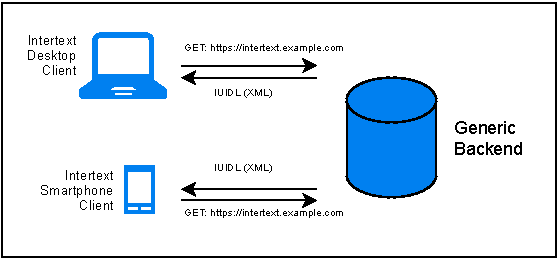
\includegraphics[width=13cm]{thesis/paper/images/how_it_works.pdf}
  \caption{A diagram showing the general workings of Intertext}%
  \label{fig:how_intertext_works}%
\end{figure}


Intertext aims to support multiple software clients (currently only the web client is implemented) built natively for various platforms that can interpret IUIDL most appropriately to the host device or platform. For instance, users browsing an Intertext app through a smartphone receive an experience optimised for touch screens, command-line interface client users receive an optimised experience for a text-based interface or a user browsing from a low-end device with limited capabilities use the version optimised for low-performance devices to get a comfortable viewing experience and so on. 

\section{Design Principles} \label{designPrinciples}

In order to address the problems mentioned in the \nameref{problemStatement} section, we adopted and implemented the following design principles.

\subsection{No Foreign Code Execution}

There is no foolproof way of entirely securing a piece of software; even the most mature platforms and operating systems sometimes end up vulnerable to security exploits. However, without the ability to execute code on a platform, it is not directly possible to take advantage of vulnerabilities, even if there is one. Furthermore, the nature of Intertext allowed us to adopt disallowing code execution as a design principle. Intertext clients only accept UIUDL code, which is in XML and is not executable. Should a server send anything else, Intertext clients will simply ignore it. Thus, we can guarantee security for the users, regardless of the platform they are using the Intertext client on.

\subsection{Transparency}

Privacy is a common concern among users; primarily due to the recent scandals and data leaks, people started getting more conscious about their data. There is an increasing demand for users to be more in control and be aware of what is exposed and what is not. In order to address this burning need, we adopted transparency as a design principle. 

The most prominent way of achieving this is to have Intertext clients in control of all interactions with the device and with external sources and keep logs in order to make them transparent to the user. The above-mentioned principle that no foreign code will be executed goes hand-in-hand with achieving this, as it would be unrealistic to expect complete control as it would be a non-deterministic approach. A good analogy would be to think of Intertext clients as an API endpoint that runs on users devices and exposes fundamental interactions with the host device and external networks through an API in a fully controlled manner. An application could \dquote{instruct} the Intertext client via IUIDL to perform some actions, such as making a network request, storing data, and accessing the local storage. An Intertext client will then block this action until the user grant permission and keeps a log every time before performing an action as shown in Figure~\ref{fig:permission_flow}

\begin{figure}
  \centering
  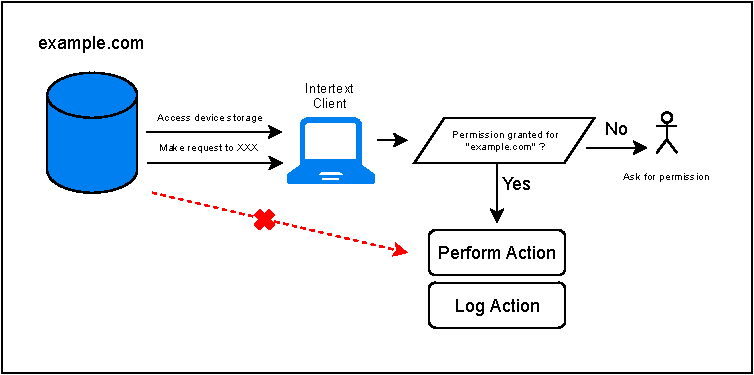
\includegraphics[width=13cm]{thesis/paper/images/permission.pdf}
  \caption{A diagram showing the permission flow}%
  \label{fig:permission_flow}%
\end{figure}


\subsection{Black-Box Components}

Intertext adopts a component-based approach with a set of components that developers can use to build their applications. Each component accepts a set of properties, which gives them certain functionality or appearance. Developers are to use these components through the IUIDL. For example, the IUIDL code shown in Figure~\ref{fig:iuidl_buttons} and its output for the Intertext web version shown in Figure~\ref{fig:iuidl_buttons_output} shows some of the properties that a \texttt{button} component accepts. Layout properties such as \texttt{marginButton} allows positioning of the buttons to be customised, \texttt{intent} properties gives the button a different look based on the use case, properties like \texttt{disabled} can alter its behaviour and so on.

\begin{figure}[htb]
\begin{minipage}{\linewidth}
\begin{lstlisting}[language=xml]
<h3>Buttons</h3>
<grid cols="[1,1]">
  <block>
    <button marginBottom="2">default</button>
    <button marginBottom="2" disabled="true">disabled</button>
  </block>
  <block>
    <button marginBottom="2" intent="default">default</button>
    <button marginBottom="2" intent="primary">primary</button>
    <button marginBottom="2" intent="error">error</button>
    <button marginBottom="2" intent="warning">warning</button>
    <button marginBottom="2" intent="success">success</button>
    <button marginBottom="2" intent="info">info</button>
  </block>
</grid>
\end{lstlisting}
\end{minipage}
\caption{UIUDL that renders buttons in several states}%
\label{fig:iuidl_buttons}%
\end{figure}

\begin{figure}[htb]
  \centering
  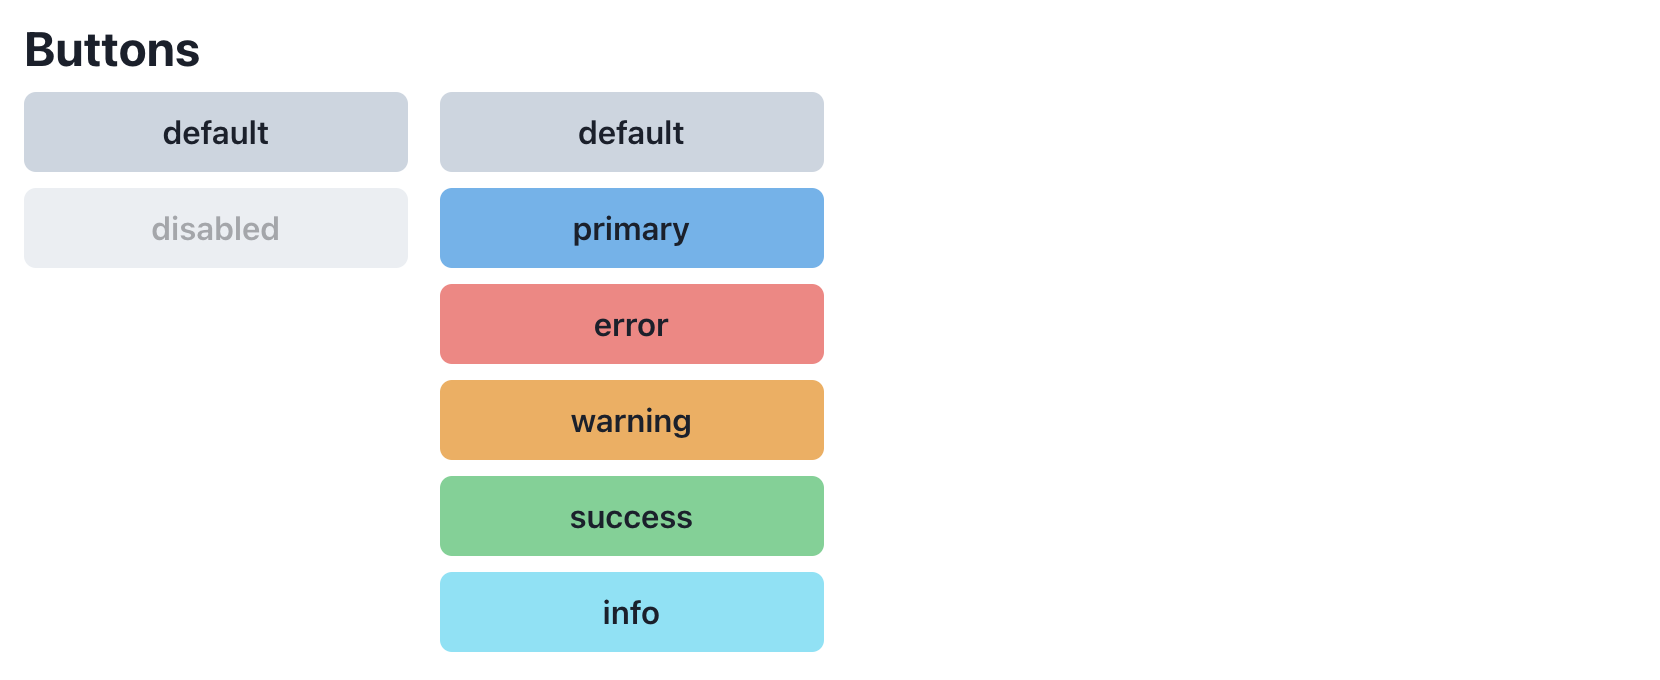
\includegraphics[width=13cm]{thesis/paper/images/buttons.png}
  \caption{Output of IUIDL in Figure~\ref{fig:iuidl_buttons} on Intertext web client}%
  \label{fig:iuidl_buttons_output}%
\end{figure}

However other than properties that components accept, they cannot be modified or altered by the developer. The main motive behind this principle is standardisation. When all Intertext applications use the same set of components, we can control how they look and how they are implemented, and ensure certain behavioural and visual aspects to bring the benefits in order to solve some of the problems mentioned in the problem statement.

Consistency is one of the most important benefits that this principle enables. A standard look and feel in components prevents users from getting disoriented across applications, and recognise similar patterns. Another benefit is customisability. It is only possible to create one-size-fits-all themes that apply to every component in every application when all the applications uses components that are built in the same way. Another thing that comes to mind is accessibility. We mentioned in Section~\ref{problemStatement} that accessibility is a big issue that not all developers choose to address. This principle allows us to take this responsibility from the developers' hands by providing accessible components as building blocks. 

Last but not least, this principle was crucial to achieve cross-device compatibility. The appearance and behaviour of components differs between implementations of the Intertext clients. For instance, the \texttt{button} component on the web version does not need to be too big as clicks are precise, and it requires a hover and focus state. For a touch interface however, it needs to be bigger, and handle the caveat of having less precision by accepting hits on an area around it. Every feature that components have needs to be supported as much as possible on different platforms that has different requirements. Having components with a fixed set of features allowed us to implement them all for different Intertext clients.

\subsection{Shared Syntax}

We designed the IUIDL to be a generic markup language, agnostic of any platform or interaction type, and be based purely on XML so it could be consumed by all clients. This approach has many advantages, both for developers and users. It allows developers to create universal applications; once they start serving an Intertext application through an endpoint, any Intertext endpoint can consume the application through that endpoint. Moreover, it helps creating a continual experience for the user; given that there is a shared layout system, UI elements will look and feel the same between Intertext clients.

Also, this approach allows existing Intertext applications to adopt to new Intertext clients as they are built in the future. At the time of writing this paper, only the Intertext web client is ready. Thanks to this principle, upcoming Intertext clients will have immediate availability.

\section{Intertext UIDL} \label{intertextUIDL}

The Intertext UIDL (IUIDL) is an XML-based markup language that can be used to describe user interfaces. It features a layout system and UI components that could be used as building blocks to put together a user interface. IUIDL is meant to be served from a generic backend, assembled on the backend based on the application logic. It is designed to be unopinionated, as it does not restrict how you assemble it or serve it, or where you serve it from. For instance, below is an example To-do list UI served in IUIDL from a Node.js server that uses Express.js framework, as shown in Figure~\ref{fig:todos_js}. Once requested, the endpoint \texttt{/todo} passes the To-do item data to a template file which uses Handlebars as a template engine, and it renders the UI in IUIDL format. The XML output is served from the endpoint.

\begin{figure}[htb]
\begin{minipage}{\linewidth}
\begin{lstlisting}[language=javascript]
router.get('/todo', function(req, res, next) {
  const todos = [
    { title: 'Buy milk', done: false },
    { title: 'Call mom', done: false },
    { title: 'Prepare for presentation', done: true },
  ];
  res.render('todo', {
    itemsToDo: todos.filter(item => !item.done),
    itemsDone: todos.filter(item => item.done),
  });
});
\end{lstlisting}
\end{minipage}
\caption{A simple Express endpoint that serves the render output of the Handlebars template shown in Figure~\ref{fig:todos_template}}%
\label{fig:todos_js}%
\end{figure}

\begin{figure}
\begin{minipage}{\linewidth}
\begin{lstlisting}[language=xml]
<h3>To do ({{ itemsToDo.length }})</h3>

{{#each itemsToDo}}
  <block intent="default" flexDirection="row" alignItems="center" paddingLeft="4">
    <text flexGrow="1">{{this.title}}</text>
    <button intent="error">Remove</button>
    <button intent="success" marginLeft="2">Done</button>
  </block>
{{/each}}


<h3>Done ({{ itemsDone.length }})</h3>

{{#each itemsDone}}
  <block intent="default" flexDirection="row" alignItems="center" paddingLeft="4">
    <text flexGrow="1">{{this.title}}</text>
    <button intent="error">Remove</button>
  </block>
{{/each}}
\end{lstlisting}
\end{minipage}
\caption{Handlebars template that renders To-do items in IUIDL format}%
\label{fig:todos_template}%
\end{figure}

\begin{figure}
  \centering
  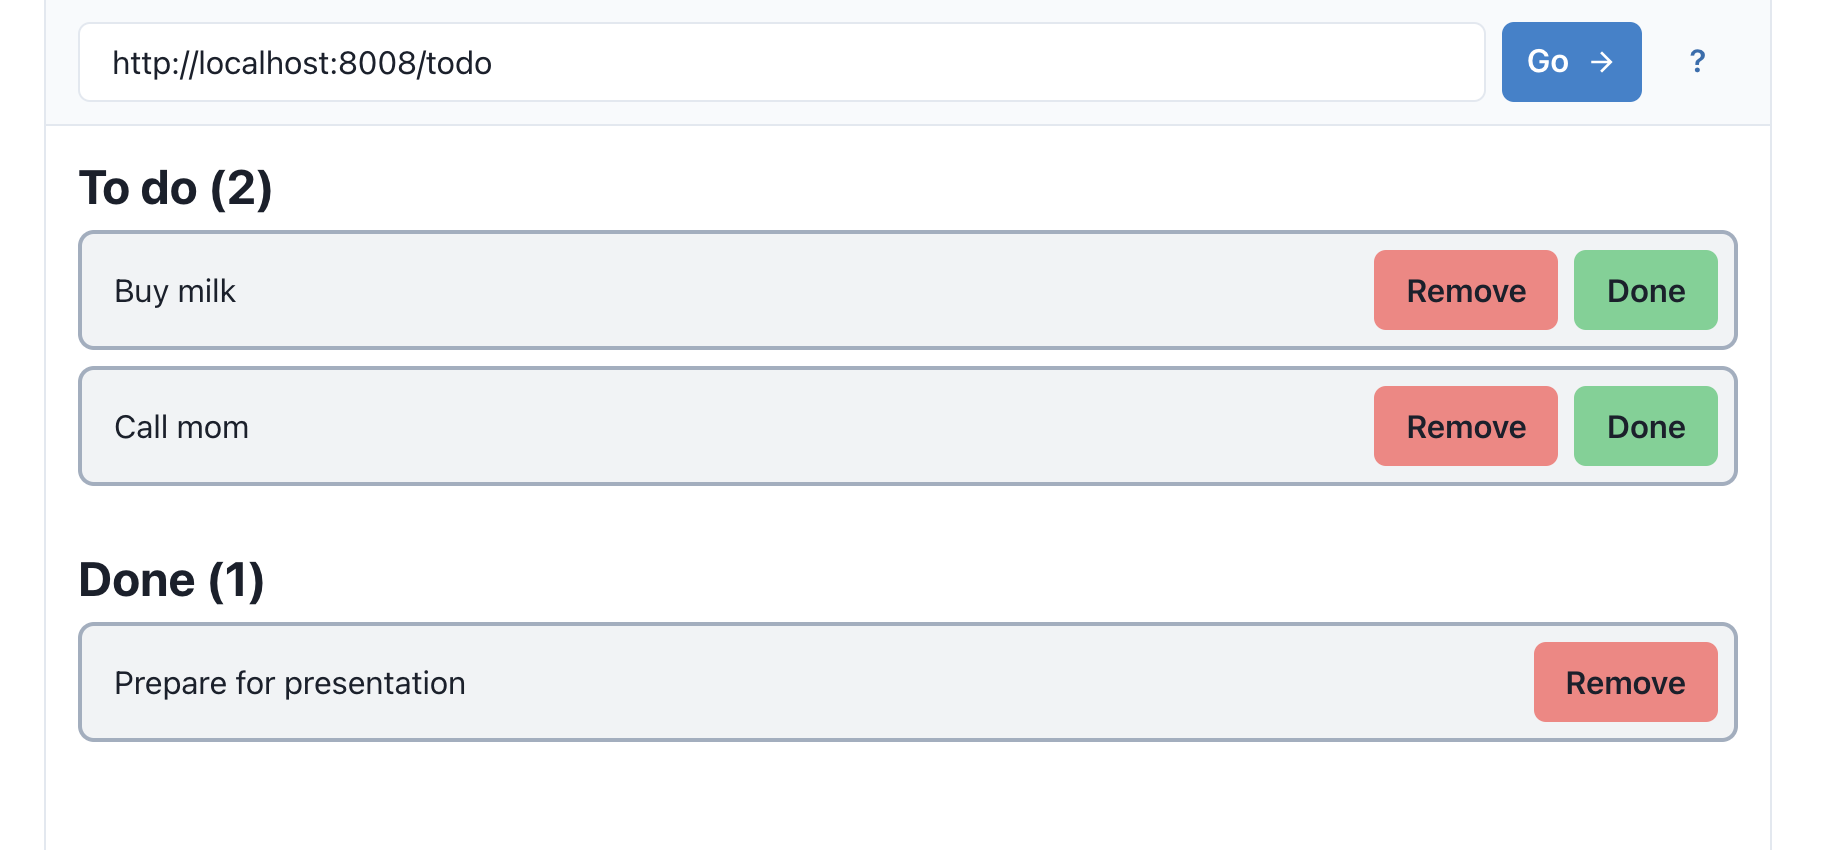
\includegraphics[width=13cm]{thesis/paper/images/todos.png}
  \caption{IUIDL served from the endpoint in Figure~\ref{fig:todos_js} rendered by the Intertext web client}%
  \label{fig:todos_output}%
\end{figure}

\subsection{Styling}

IUIDL is agnostic of the styling. There are several \textit{intent}s that components can accept, which renders the component most appropriately based on its use case. For instance, the Remove buttons in Figure~\ref{fig:todos_output} as can be seen as red, and Done buttons green. That is because the \textit{error} intent was given to the Remove button and \textit{success} intent was given to the Done button. However, in this configuration, there is no way to specify how the components look like in particular. The main idea is customisability. Intertext provides themes that users can choose from, and for each theme UI components look and feel differently. Currently, only light and dark themes are available for the web version of Intertext (the dark version of the To-do list UI can be seen in Figure~\ref{fig:todos_output_dark}), but as mentioned in the \nameref{futureWork} section, more themes will be made available. Moreover, users will also be able to create custom themes that exactly match their liking.

\begin{figure}
  \centering
  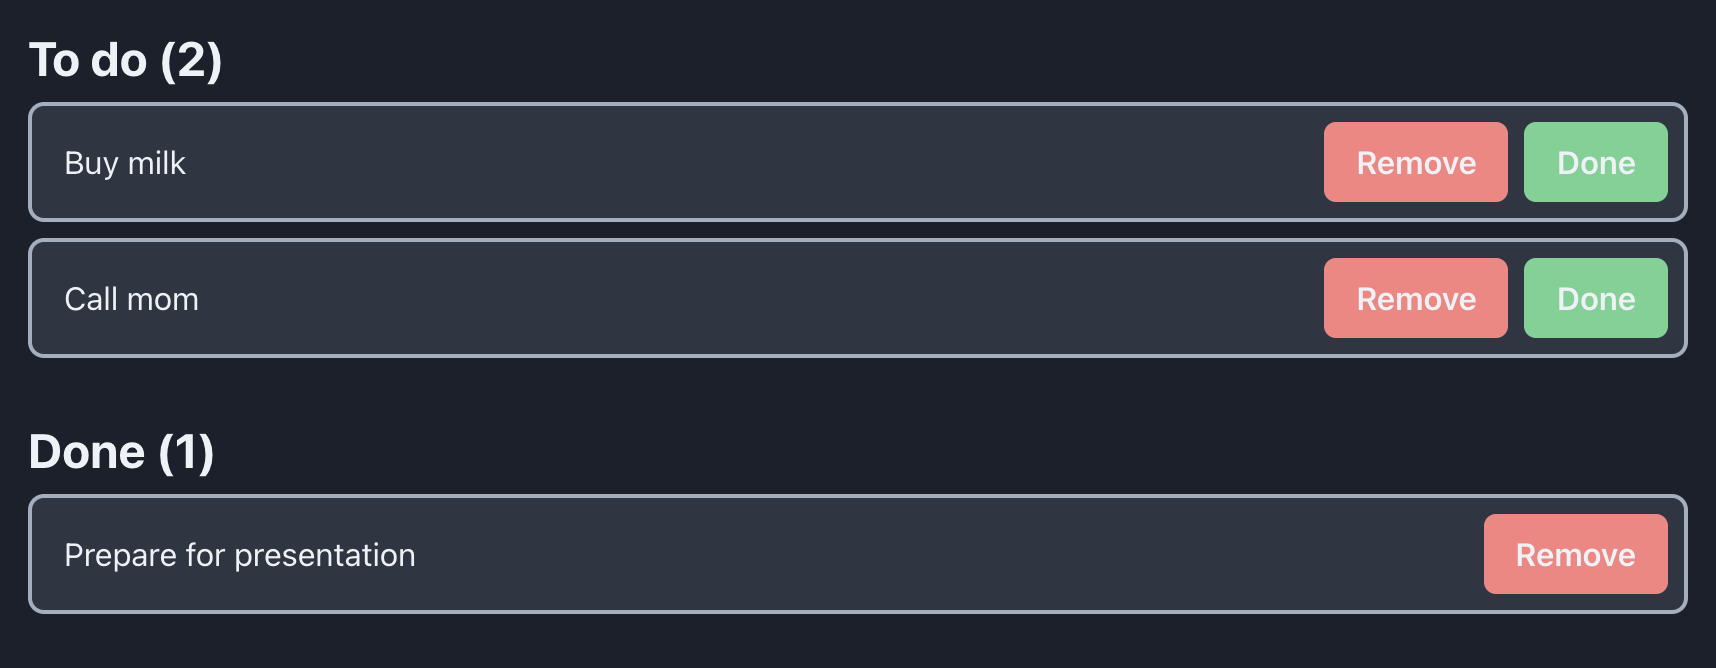
\includegraphics[width=13cm]{thesis/paper/images/todos_dark.png}
  \caption{Dark version of the To-do list UI from Figure~\ref{fig:todos_output} rendered by Intertext web client}%
  \label{fig:todos_output_dark}%
\end{figure}

\subsection{Syntax}

As explained in detail in the \nameref{implementation} section, IUIDL gets converted from XML syntax to JSON syntax. However, the conversion to JSON is only an implementation detail that takes place during the rendering phase, and developers do not need to be aware of. XML was chosen at the cost of creating an additional transpilation layer, to achieve optimum developer friendliness. 

\begin{figure}[htb]
\begin{minipage}{\linewidth}
\begin{lstlisting}[language=xml]
<block intent="error">
  <h3 intent="error">Not Found</h3>
  <collapse>
    <collapse.handle>
      <text intent="error">
        Show Details
      </text>
    </collapse.handle>
    <p intent="error">... stack trace here ...</p>
  </collapse>
</block>
\end{lstlisting}
\end{minipage}
\caption{The XML representation of the 404 page}%
\label{fig:syntax_xml}%
\end{figure}

When it comes to building UIs, XML and XML-like languages are very common. The main benefit of such languages is that they are easy to read and write, while at the same time they are easy to parse and process as data. IUIDL is meant to be served from a backend, but developers still need to write IUIDL code by hand on the server side. JSON is far from being practical to write in large by hand. The difference could be observed in Figure~\ref{fig:syntax_json} and Figure~\ref{fig:syntax_xml}, where the IUIDL code for a custom 404 page is shown in both XML and JSON syntax.

\begin{figure}[htb]
\begin{minipage}{\linewidth}
\begin{lstlisting}[language=json]
[
  {
    "block": [
      { "h3": "Not Found", "intent": "error" },
      {
        "collapse": [{
          "p": "... stack trace here ...",
          "intent": "error"
        }],
        "handle": [{
          "text": "\n Show Details\n",
          "intent": "error"
        }]
      }
    ],
    "intent": "error"
  }
]
\end{lstlisting}
\end{minipage}
\caption{The JSON representation of the 404 page}%
\label{fig:syntax_json}%
\end{figure}


One issue that raised from the XML syntax was the inability to assign complex children to attributes of a specific tag. As it can be seem from the JSON representation of the 404 page in Figure~\ref{fig:syntax_json}, the component \texttt{collapse} requires two sets of children: one for its direct children (specified as \texttt{collapse}), and one for the children to be rendered in its handle (specified as \texttt{handle}). Both \texttt{collapse} and \texttt{handle} properties take other UI components as their children. However, the XML syntax only allows attribute values of an element to be a string. In order to solve this problem, we introduced a special tag name convention: when an XML tree is placed as the children of a component with the tag name being the parent components name concatenated with an attribute name joined together with a dot (\dquote{.}), it gets interpreted as an attribute of the parent, with its value being the children of that XML tree as shown in Figure~\ref{fig:complex_attributes}.

\begin{figure}[htb]
\begin{minipage}{\linewidth}
\begin{lstlisting}[language=xml]
<a>
  <a.b>
    <text>
      This is under 'b' attribute of the parent 'a'
    </text>
  </a.b>
  <text>
    This is the real children of parent
  </text>
</a>
\end{lstlisting}
\end{minipage}
\caption{Complex attributes}%
\label{fig:complex_attributes}%
\end{figure}


\subsection{Terminology}

A last thing to mention in this section is the terminology used in IUIDL. The IUIDL syntax is shared between multiple devices and environments, which includes desktop interfaces as well as touch interfaces, non-graphical user interfaces and more. As mentioned in the \nameref{futureWork} section, when more Intertext clients get released, the variety will further increase. This brings up a problem with the terminology. For instance, the \texttt{click} that normally would make sense for a desktop environment does not make sense for touch interfaces, as the interaction for a touch screen interface would be \texttt{touch} or \texttt{tap}. In the case of a command-line interface, the primary interaction is focusing on an item and hitting the \texttt{enter} key. 

Our immediate reaction to solve this problem was to create custom jargon that is agnostic of device/interaction type, just like IUIDL is by nature, and find terms for every component/interaction that apply globally. For instance, instead of \texttt{button} we used \texttt{callToAction}, and instead of \texttt{onClick} we used \texttt{onPrimaryInteraction}. However we later abandoned this approach for the sake of developer friendliness. As we custom-named components and their respective actions, we realised that their names were getting very unusual and non-familiar, to a point where it was very difficult to even recognise them. Should we have chosen the global naming convention, we would have introduced a steep learning curve; developers would have needed to get familiar with a long list of terms that they have never heard of before, and they would strictly need to follow the documentation while building Intertext applications.

Instead, we decided to adopt the terminology for desktop/web environments. The rationale behind this decision was that these environments have been around for a very long time, that the terms used to build desktop applications and web applications have a strong recognition among many developers. Also, terms used for desktop environments were mostly generic enough that it was easy to represent them in other environments. For instance, a \texttt{button} is a component to be interacted with that performs an action, and \texttt{click} is the method of primary interaction with that component. We can easily take this as a given to replicate it on any environment and create an optimised version taking the limitations of the host platforms in mind.

\section{Intertext Clients} \label{intertextClients}

Intertext clients are the user facing products of Intertext, that build the bridge between the user and servers that serve IUIDL. They are meant to be implemented natively for the host platform in the most optimal way possible. 

For example, on mobile platforms such as iOS and Andriod, UI elements would be larger and more suitable for touch interactions. Primary interaction would be translated as \texttt{tap} while secondary interactions, if any, would be translated as \texttt{tap and hold}. The layout would adjust itself based on the screen size. The client would be implemented with either native technologies such as Swift/Objective-C for iOS and Kotlin/Java for Android, or with hybrid technologies that get compiled into native code, such as React Native or Flutter for maximum responsiveness and efficiency. 

At the time of writing this paper, only a web client has been implemented. A command-line client, native clients for iOS and Android, and desktop clients for Mac OS, Windows and several Linux distributions are among the ones that are planned, as detailed in the \nameref{futureWork} section.

Intertext clients consist of two main parts, components and commands. Each Intertext client implements these separately, based on the host platform and its capabilities. Each client also implements their own local storage, state management strategy, and communication technique with the server.

\subsection{Components}

Components are anything that has a visual representation. All components stem from a generic IUIDL definition, and are interpreted based on the host platform requirements. They can be organisational or presentational. Organisational components are the layout components, they are used to position presentational components on the screen. Intertext implements a version of the CSS flexbox specification as a layout system, which could be used to implement responsive interfaces for all screen sizes. For non-browser-based platforms, we use the popular Yoga layout engine\footnote{\url{https://yogalayout.com}}, which is a standalone implementation of the css flexbox specification in C++, allowing us to target almost any platform. More details on the layout system is given in the \nameref{implementation} section.

Most presentational Intertext components share a concept, \texttt{intent}, which is a way to communicate the intention of the UI element based on its use-case. Intertext clients render the UI elements differently based on its intent, allowing a way for the developer to convey an intention of an UI element to the user without being able to intercept with the styles. For instance, an error message could be shown in a block component that has the intent \texttt{error}, and it will be rendered with a red background, indicating to the user that it is an error message. Figure~\ref{fig:intents} shows an example of intents on block component for Intertext web client.

\begin{figure}[htb]
  \centering
  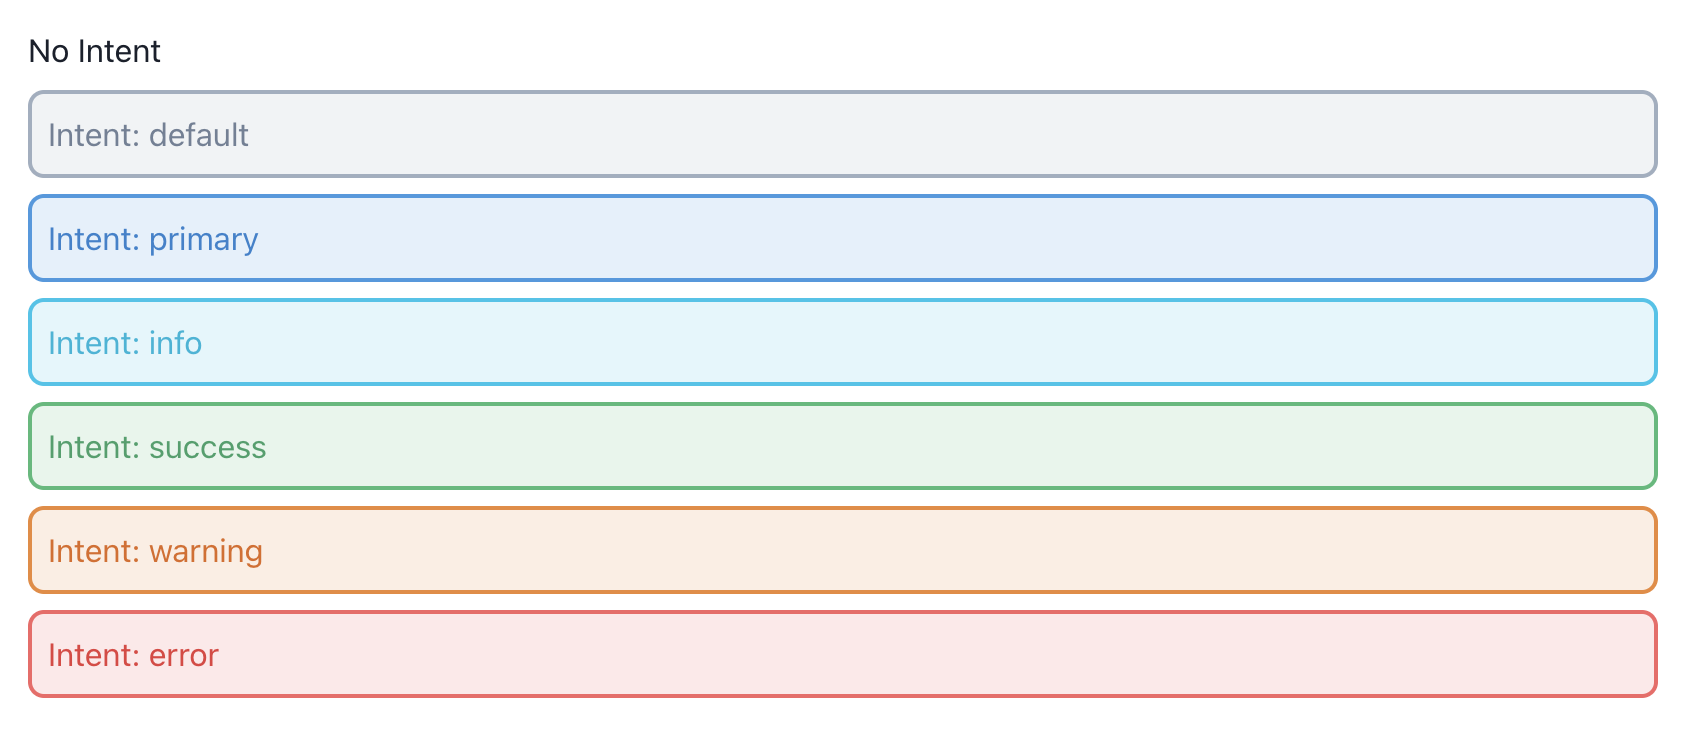
\includegraphics[width=13cm]{thesis/paper/images/intents.png}
  \caption{Intents for Block components}%
  \label{fig:intents}%
\end{figure}

\subsection{Commands}

Commands are IUIDL statements that are used to instruct Intertext clients to take an action. These actions can be triggered upon interaction with some components (such as clicking a button or submitting a form), a life-cycle event, with a timeout, or on page load. Commands are primitive by design, they are not meant to build application logic with. They are merely for asking the Intertext client to communicate with the server, store something, read something that is stored, or retrieve some user data. Command system is designed in order to ensure Intertext client is aware of what it is being asked to do, so that it can control and restrict the entire flow, ask for permission from the user when necessary, or simply refuse to take an action if needed. 

\begin{figure}[htb]
\begin{minipage}{\linewidth}
\begin{lstlisting}[language=xml]
<timeout delay="1000">
  <request endpoint="/refresh"></request>
</timeout>
\end{lstlisting}
\end{minipage}
\caption{Post command on Timeout}%
\label{fig:ex_cmd_post_timeout}%
\end{figure}

Figure~\ref{fig:ex_cmd_post_timeout} shows an example of how a network request action can be executed upon a delay, and Figure~\ref{fig:ex_cmd_form} shows how a form can be submitted with reference to input fields. More on commands will be on \nameref{implementation} section.

\begin{figure}[htb]
\begin{minipage}{\linewidth}
\begin{lstlisting}[language=xml]
<input name="item_title"></input>
<input name="item_description"></input>
<button>
  <text>Submit</text>
  <button.onClick>
    <request endpoint="/items/save"></request>
  </button.onClick>
</button>
\end{lstlisting}
\end{minipage}
\caption{Form command with reference on server side to internal input values}%
\label{fig:ex_cmd_form}%
\end{figure}

\begin{figure}[htb]
\begin{minipage}{\linewidth}
\begin{lstlisting}[language=javascript]
router.get('/signup', async (req, res, next) => {
  
  const currentStep = req.body.state?.current_step ?? 0
  const currentInputState = req.body.inputState
  const previousInputState = req.body.state.input_state
  
  // check if user finished the form
  if (currentStep == LAST_STEP) {
    // execute signup logic
    const error = await signupUser(req.body.state?)
    // render success or error page based on
    // the signup result
    res.render(error
      ? 'signup_form_error'
      : 'signup_form_success',
    { error });
  } else {
    // render signup form
    res.render('signup_form', {
      // increment the current step
      step: currentStep + 1
      // merge current form data with previous
      inputState: merge(
        previousInputState,
        currentInputState
      )
    });
  }
});
\end{lstlisting}
\end{minipage}
\caption{Handling a sign-up flow with multiple steps}%
\label{fig:state_signup_progress_js}%
\end{figure}

\subsection{State Management}

Intertext clients offer some basic state management, making it possible to serve stateful Intertext applications using serverless/stateless backends. front-end state can be fully driven from the backend via IUIDL. Intertext client offers two types of storage, persisted and volatile. 

Volatile storage is kept in the memory and persisted across the session. The purpose of this storage is to keep temporary values, such as users' progress in a long form distributed across multiple pages. Intertext clients pass the entire application state of the volatile storage to the backend with every request, allowing the backend to build logic around the current state of the front-end application, and serve the UI accordingly. Figure~\ref{fig:state_signup_progress_js} and Figure~\ref{fig:state_signup_progress_xml} show this through a hypothetical sign up form with sign up steps distributed across multiple screens. Figure~\ref{fig:state_signup_progress_js}, we see the pseudo-code implementation of the stateless backend for this scenario. It can be seen that the current step user is at, and the input state data collected thus far is kept in the volatile state on the front-end. The state gets passed on to the backend on every request made to the \texttt{/signup} endpoint. We retrieve the current step, and serve different responses accordingly. If a user completed the last step, then we execute our application logic (which in this case is signing user up), and render the result page. Otherwise, we increment the current step, combine the form data collected thus far, and render the form template with these. On the form template in Figure~\ref{fig:state_signup_progress_xml}, we use the \texttt{<state>} block to instruct the Intertext client to record these new set of data to the front-end, so it could be passed on to the backend on the next request. Moreover, we render the correct form UI based on the step user is currently at.

\begin{figure}[htb]
\begin{minipage}{\linewidth}
\begin{lstlisting}[language=xml]
<!-- signup_form -->

<!-- set front-end state to read on later requests  -->
<state key="current_step">{{ step }}</state>
<state key="input_state">{{ inputState }}</state>

{{#ifEquals step 1}}
  <!-- form elements for step 1 -->
{{/ifEquals}}

{{#ifEquals step 2}}
  <!-- form elements for step 2 -->
{{/ifEquals}}

<!-- ... -->
\end{lstlisting}

\begin{lstlisting}[language=xml]
<!-- signup_form_success -->

<h1 intent="success">Sign Up Successful!</h1>
<p intent="success">Please check your verification email</p>
\end{lstlisting}

\begin{lstlisting}[language=xml]
<!-- signup_form_error -->

<h1 intent="error">Something went wrong</h1>
<p intent="error">{{error}}</p>
\end{lstlisting}

\end{minipage}
\caption{Template files for multi-step sign up flow in Figure~\ref{fig:state_signup_progress_js}}%
\label{fig:state_signup_progress_xml}%
\end{figure}

Another type of storage is the persisted storage. As the name suggests, values stored this way are persisted across sessions. Unlike the volatile storage, in which the data is kept in the memory, persisted storage gets stored locally using the storage option available to the host platform. By default, data available in the persisted storage is not passed on to the backend in every request automatically, but can be configured to do so.

In order to protect user privacy, Intertext clients block cross-origin storage reads/writes, preventing users to be tracked across Intertext applications. In another words, state management is bound to the origin. Lets assume \texttt{sub1.example.com} wrote data to the storage. This data can only be read or manipulated by the very same domain. \texttt{sub2.example.com} or \newline\texttt{sub.example2.com} or any other domain will not have access to this data. While this behaviour protects users from cross-origin tracking, it may also be inconvenient for some users, especially in scenarios such as services that share the same user login that is distributed across multiple domains/subdomains. As further mentioned in the \nameref{futureWork} section, we plan to add a feature where Intertext clients would ask for user permission to share data between domains/subdomains instead of directly blocking it.


% !TEX root = ../thesis.tex

\chapter{Implementation} \label{implementation}

The primary language used to implement Intertext is TypeScript. TypeScript is a superset of JavaScript that brings typing support for safety and a better developer experience. TypeScript gets transpiled into JavaScript during build time, therefore the byproduct is plain JavaScript. Sharing the same language between Intertext clients brings a number of advantages, mostly code sharing.

\section{Engine}

Code sharing between Intertext clients for several reasons has been an important priority while creating the architecture. First of all, it is crucial for Intertext clients to behave consistently for some tasks that are common to every Intertext client, such as the parsing of IUIDL, rendering of the components, behavioural aspects of the clients, the data structure and so on. These are the cornerstone of Intertext, and they must behave exactly the same across clients. In other words, everything that is not client-specific needs to be consistent and predictable. This is where the Intertext engine comes in play.

The Intertext engine implements several aspects of Intertext clients; most notably it parses IUIDL, internally converts it into JSON, and uses the output to render the components. Intertext clients are only concerned with the view layer, but they use the engine as a black box system. The engine also defines the data types of every component, and the internal mechanics of the build and rendering process. It exposes the types for Intertext clients built with TypeScript to consume. Intertext engine is built as a standalone library, it exposes the main functions and types, and it is designed to be used in several different ways.

At the time of writing, all Intertext clients that are implemented so far were built with TypeScript; they simply import and use the engine as a dependency. Their build system picks up the engine and adds it to their final bundle. However this approach is not possible for potential future clients that do not built on a JavaScript runtime. To overcome this issue, the engine can be compiled as a Node module, and be deployed to a Node.js server. This gives us the ability to use the engine on any software system that can send or receive HTTP requests. Moreover, with the same logic, the engine can be deployed locally alongside any Intertext client that runs on a platform that can support Node.js runtime. It can then be deployed and served locally, and used to communicate with the local Intertext client using any protocol that is supported by the host platform as long as there exists a data exchange. 

For instance, say a car manufacturer wanted to build an Intertext client for their in-car entertainment system using their own components. They could potentially install Node.js on their computer system, or even install a simple Raspbery Pi-like chip that can run Node.js. Then, they can install the engine as a standalone application in it, and utilise any protocol to build a communication channel between the Intertext client they built on their computer system and the chip. Then, they could serve the IUIDL code either through a network connection (if and when available), or from a locally running server, potentially from the same one the client uses to interact with the engine. 

\section{Layout}

The premise of Intertext is that there will be a unified implementation of UIs, in a more or less abstract format, which will then be reified into fully functional front-ends on many different environments. These environments have different requirements and limitations, and an all-in-one solution is needed that will handle all these different requirements and limitations with minimal compromises. One of the aspects that needed consideration was the variation in screen sizes. We had to use a layout system that can be used to build a UI once, and would render properly on various screen sizes.

The obvious solution to this problem was using web technologies, as responsive design is one of the cornerstones of web development. There are many well-defined specifications in place to build UIs for different screen sizes. But we cannot directly use web technologies as many of the clients are not browser based. Therefore, we had to use an hybrid approach that can work universally.

\subsection{Layout System}

The IUIDL offers a powerful layout system based on the CSS flexbox specification. It allows developers to build responsive layouts and position UI elements with ease. Intertext web client makes use of the browser implementation of CSS flexbox specification, whereas for other non-browser based clients, Facebook's open source library Yoga \footnote{\url{https://yogalayout.com}} will be used. Yoga is a layout engine that implements css flexbox specification in C++, therefore it can be used on any ecosystem that can execute C++ to calculate the positioning of the UI elements.

\begin{figure}[H]
  \centering
  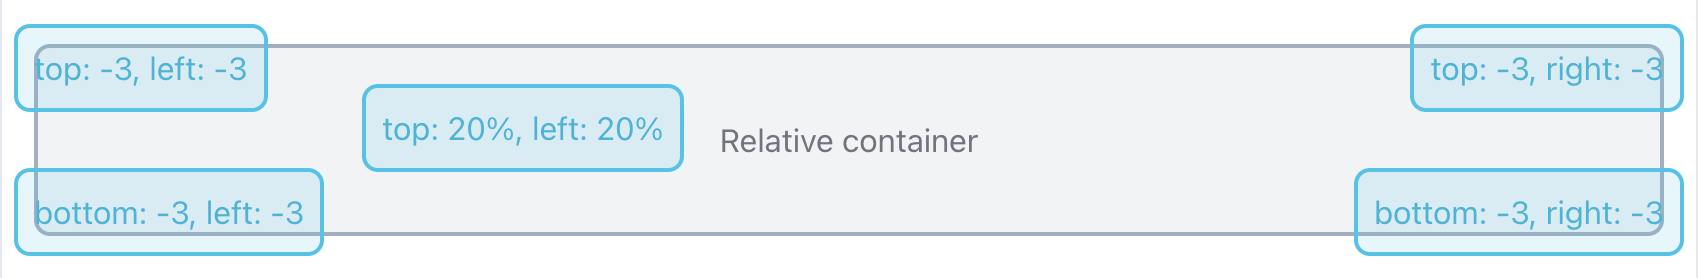
\includegraphics[width=13cm]{thesis/paper/images/absolute.png}
  \caption{Absolute positioning}%
  \label{fig:flexbox_props}%
\end{figure}

Apart from flexbox-based positioning, the Intertext layout system also supports absolute positioning. Absolute positioning detaches a component from the flow of the page and positions it relative to its first relatively-positioned parent, having it be floating over everything else, as shown in Figure~\ref{fig:absolute_positioning}.

\begin{figure}[htb]
  \centering
  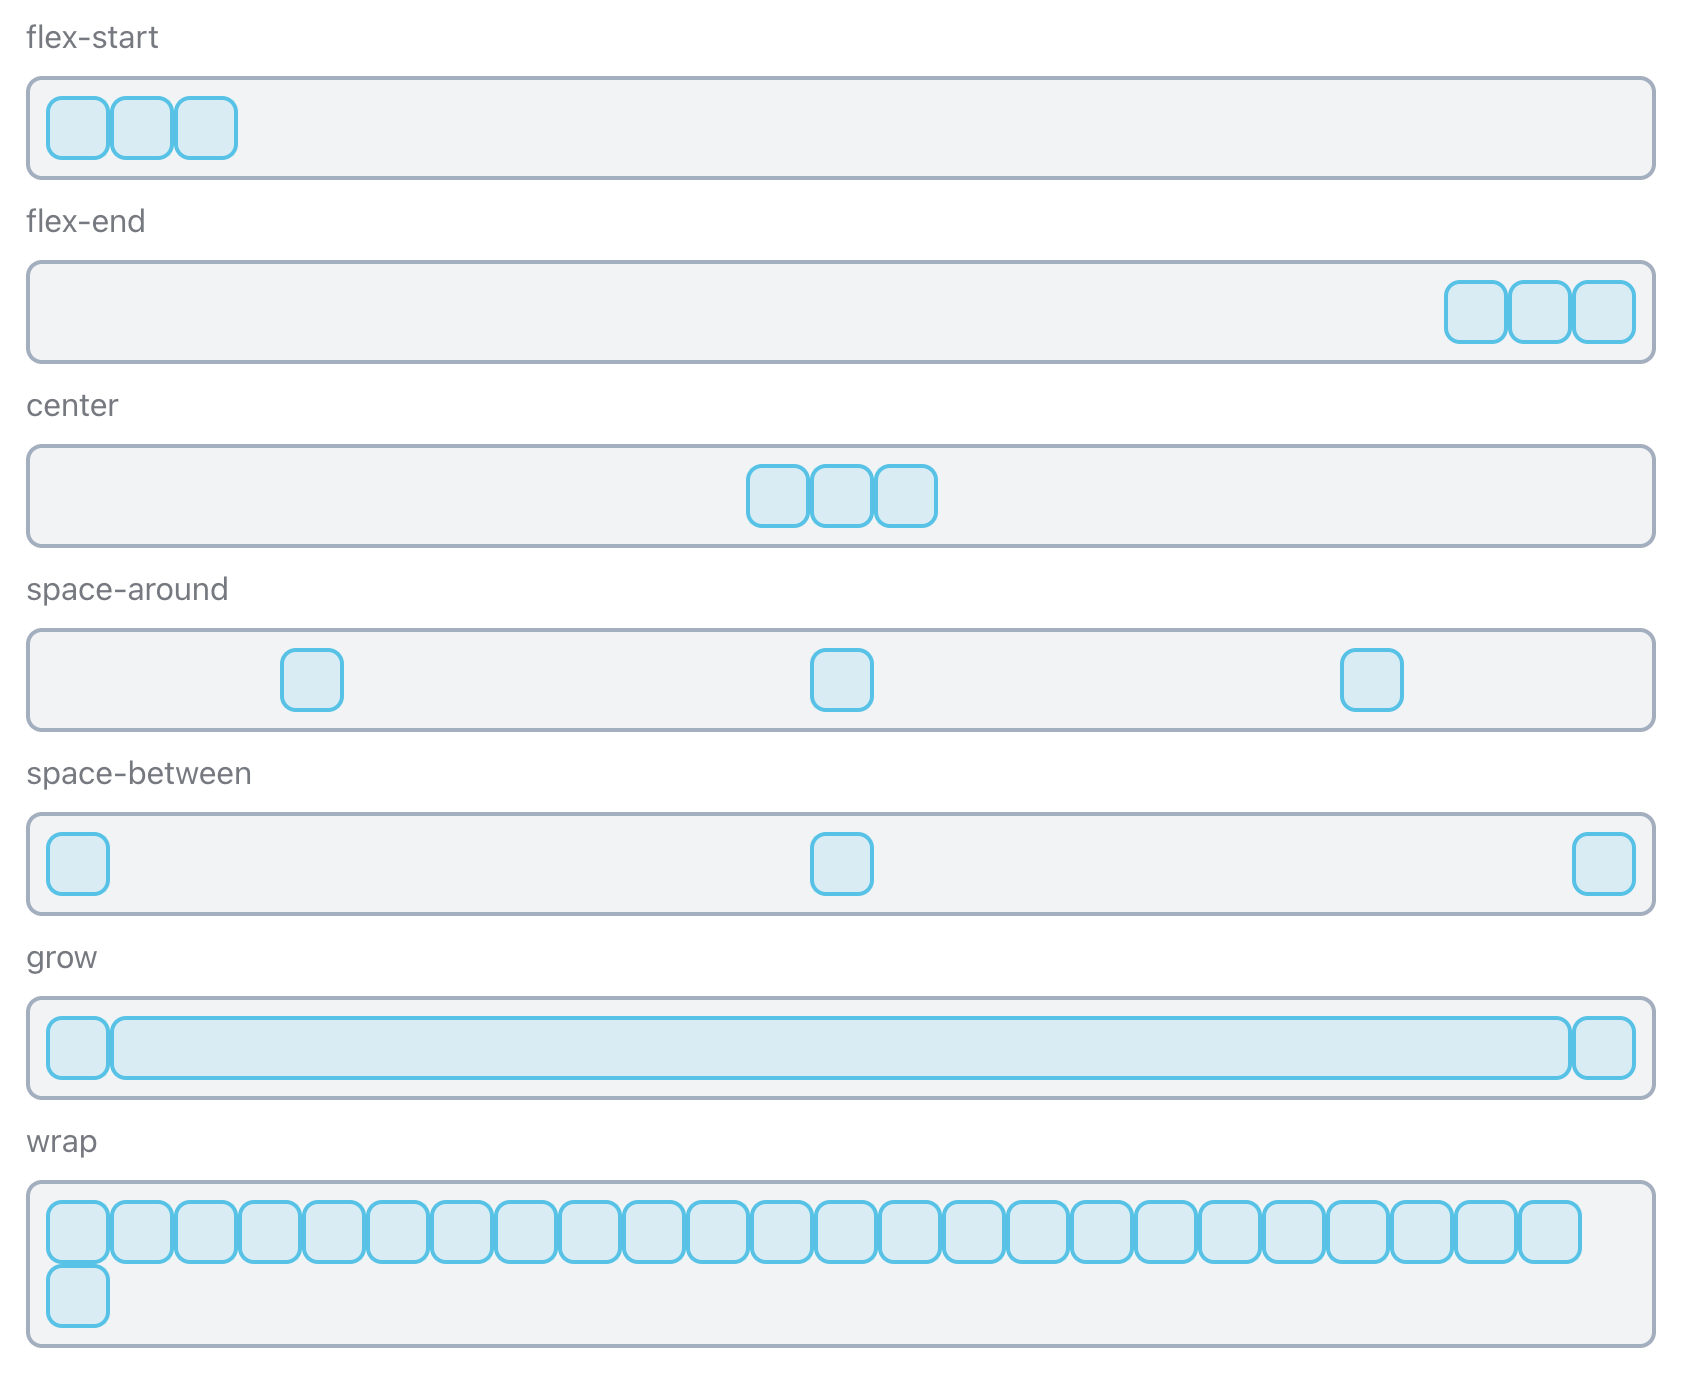
\includegraphics[width=13cm]{thesis/paper/images/responsive.png}
  \caption{Flex-box system}%
  \label{fig:absolute_positioning}%
\end{figure}

One advantage of this approach is that all our clients will render UI~elements using the same layout, which will give users a sense of familiarity when switching between the clients. For instance, when a user accustomed to using the web version of Intertext switches to, say the command-line version, they will immediately recognise the layout and be able to navigate without having to adjust. This approach will also allow developers to build responsive layouts to some extent. Given that the same UIDL code will be used to render on multiple clients, including the ones with narrow and small screens, responsiveness goes a long way. At the time of writing this paper, only flexbox features such as \texttt{flex-wrap} can be used for achieving a degree of responsiveness. However we plan to support screen size-aware variants of component properties, even conditional rendering of components based on the screen size. This can be thought of as \dquote{media queries} in css terminology. More on this will be presented in the \nameref{futureWork} section.

\subsection{Unit System}

We had to compromise a few aspects of the unit system in order to make for an all-in-one layout solution. We refrained from using definitive units that are specific to one platform, such as pixels. Most platforms use a different measurement system, for instance 1 unit for the command-line application represents a single space; character width for the x-axis and line height for the y-axis.

As a solution, we offer three different types of units; percentages, spaces and sizes. These units can be used for every property that accepts a unit; such as for the width, height, margins, paddings and so on. Percentages are universal and can be calculated on any platform that we can get the screen dimensions of. We are able to use it on the web natively, also the Yoga engine supports percentage values. Spaces are numeric values that start from 0, increments by 0.5 until 4, by 1 until 12, by 2 until 16, and keeps increasing exponentially until 96. These values are meant to be used for spacing; for paddings, margins, gutter sizes, and other cases where spaces between UI~elements needs to be determined. They are mapped to values on different platforms that are reasonable and look more or less the same. Finally, we have sizes, which are used for determining the size of UI~elements; in properties such as \texttt{width}, \texttt{height}, \texttt{minWidth}/\texttt{maxWidth}, \texttt{minHeight}/\texttt{maxHeight} and so on. While it also makes sense to use percentages for sizes, in cases where sizes should be fixed and not be changing based on the screen size, the size units can be used. Sizes are named values and are mapped to an appropriate value on every platform. They start from \texttt{3xs} (xsmall) up to \texttt{xs}, \texttt{sm} (small), \texttt{md} (medium), \texttt{lg} (large), \texttt{xl} (xlarge), \texttt{2xl} and go all the way to \texttt{8xl}.

\subsection{Properties}

\begin{figure}[htb]
\begin{minipage}{\linewidth}
\begin{lstlisting}[language=xml]
<block height="24" alignItems="center" justifyContent="center">
  <text>This is centered</text>
</block>
\end{lstlisting}
\end{minipage}
\caption{Layout properties}%
\label{fig:layout_props_example}%
\end{figure}

IUIDL defines some properties that can be used to leverage the layout system to determine the size, spacing and positioning of UI elements. Figure~\ref{fig:layout_props_example} shows an example of how layout properties can be used to center a text in a block. For positioning, \texttt{position} prop can be used, which takes \texttt{relative} or \texttt{absolute}. The default is \texttt{relative}. For spacing, supported values are \texttt{top}, \texttt{bottom}, \texttt{left}, \texttt{right}, \texttt{margin}, \texttt{marginTop}, \texttt{marginBottom}, \texttt{marginLeft}, \texttt{marginRight}, \texttt{padding}, \texttt{paddingTop}, \texttt{paddingBottom}, \texttt{paddingLeft} and \newline \texttt{paddingRight}. As for sizing, accepted values are \texttt{width}, \texttt{minWidth}, \texttt{maxWidth}, \texttt{height}, \texttt{minHeight} and \texttt{maxHeight}. All these values can take all supported unit types. To leverage the flexbox properties, the accepted properties are \texttt{alignContent}, \texttt{alignItems}, \texttt{alignSelf}, \texttt{flexDirection}, \texttt{flexWrap}, \texttt{flexGrow}, \texttt{flexShrink}, \texttt{flexBasis} and \texttt{justifyContent}. Flexbox properties follow the flexbox specification \footnote{CSS Flexible Box Layout Module Level 1: \url{https://www.w3.org/TR/css-flexbox-1}}. All layout properties mentioned above are accepted by and can be used with every Intertext component.

\section{Components}

Components are the building blocks of Intertext applications, and consist of a set of pre-defined building blocks provided out of the box, which can be assembled to create a functional front-end application. They define the view layer, and they are handled differently on every Intertext client. While the rendering logic and flow of the components are fully driven by engine for consistency, it exposes functions for Intertext clients to register renderers for each component. The renderer function gets called by the engine during the render flow; it receives the props that are the given to the component, the children of the component (if any) that the function is expected to be passing on to the next call level of the recursive rendering flow, and are expected to return the component instance that needs to be rendered, which will later be used to render the UI. Figure \ref{fig:registering_renderer} shows an example snippet of the block renderer being registered to the engine on Intertext web client.

\begin{figure}
\begin{minipage}{\linewidth}
\begin{lstlisting}[language=javascript]
import Engine from "@intertext/engine"
import Block from "../components/core/Block/Block"

const engine = new Engine()

engine.renderer.registerBlockRenderer(({
  index,
  children,
  props,
}) => (
  <Block key={index} {...props}>
    {engine.renderer.render({ branch: children })}
  </Block>
))
\end{lstlisting}
\end{minipage}
\caption{Registering a component renderer}%
\label{fig:registering_renderer}%
\end{figure}

\subsection{Block}

Block component is the most basic and primitive building block of Intertext. It can be thought of as the \texttt{div} element of HTML, its main purpose is to enclose components and other blocks. It is primarily a layout component, as it can group and position elements together. Moreover, it can also be used as a display component by accepting the \texttt{intent} property. When an intent is provided, it renders the block appropriately, thus it can be also used to convey a message. They also accept all layout properties. Figure \ref{fig:intents} shows an example of the block component on the web client, with and without intents.

\subsection{Grid}

Grid is an another layout component that can be used to render its children in grid formation. It accepts \texttt{cols} property, which can be used to define how many columns should the grid have, and what the size of the column should be. It accepts numeric values inside curly brackets delaminated with a comma. Number of items in curly brackets represents the number of columns, and each number represents units that the columns should take up, where the total number of units is the sum of the numbers inside curly brackets. For instance, if \texttt{cols} value was \texttt{[1, 1, 1, 1]}, it would mean that the grid has four columns that are divided equally, where \texttt{[1, 3]} would represent two columns with widths being 25\% to 75\%. Grid component also takes a \texttt{gap} property to describe the gutter size. It can take any one of the spacing values. Any number of children can be provided to the grid component, without the need to next them in any way, it will automatically position its immediate children based on the given configuration. Figure~\ref{fig:grid_xml} shows an example of how grid component can be used, and Figure~\ref{fig:grid} shows some render outputs of the grid component for the web client.

\begin{figure}[htb]
\begin{minipage}{\linewidth}
\begin{lstlisting}[language=xml]
<grid cols="[2, 3, 1]" gap="2">
  <block intent="info">2</block>
  <block intent="info">3</block>
  <block intent="info">1</block>
  <block intent="info">2</block>
  <block intent="info">3</block>
  <block intent="info">1</block>
</grid>
\end{lstlisting}
\end{minipage}
\caption{How grid component is used}%
\label{fig:grid_xml}%
\end{figure}

\begin{figure}[htb]
  \centering
  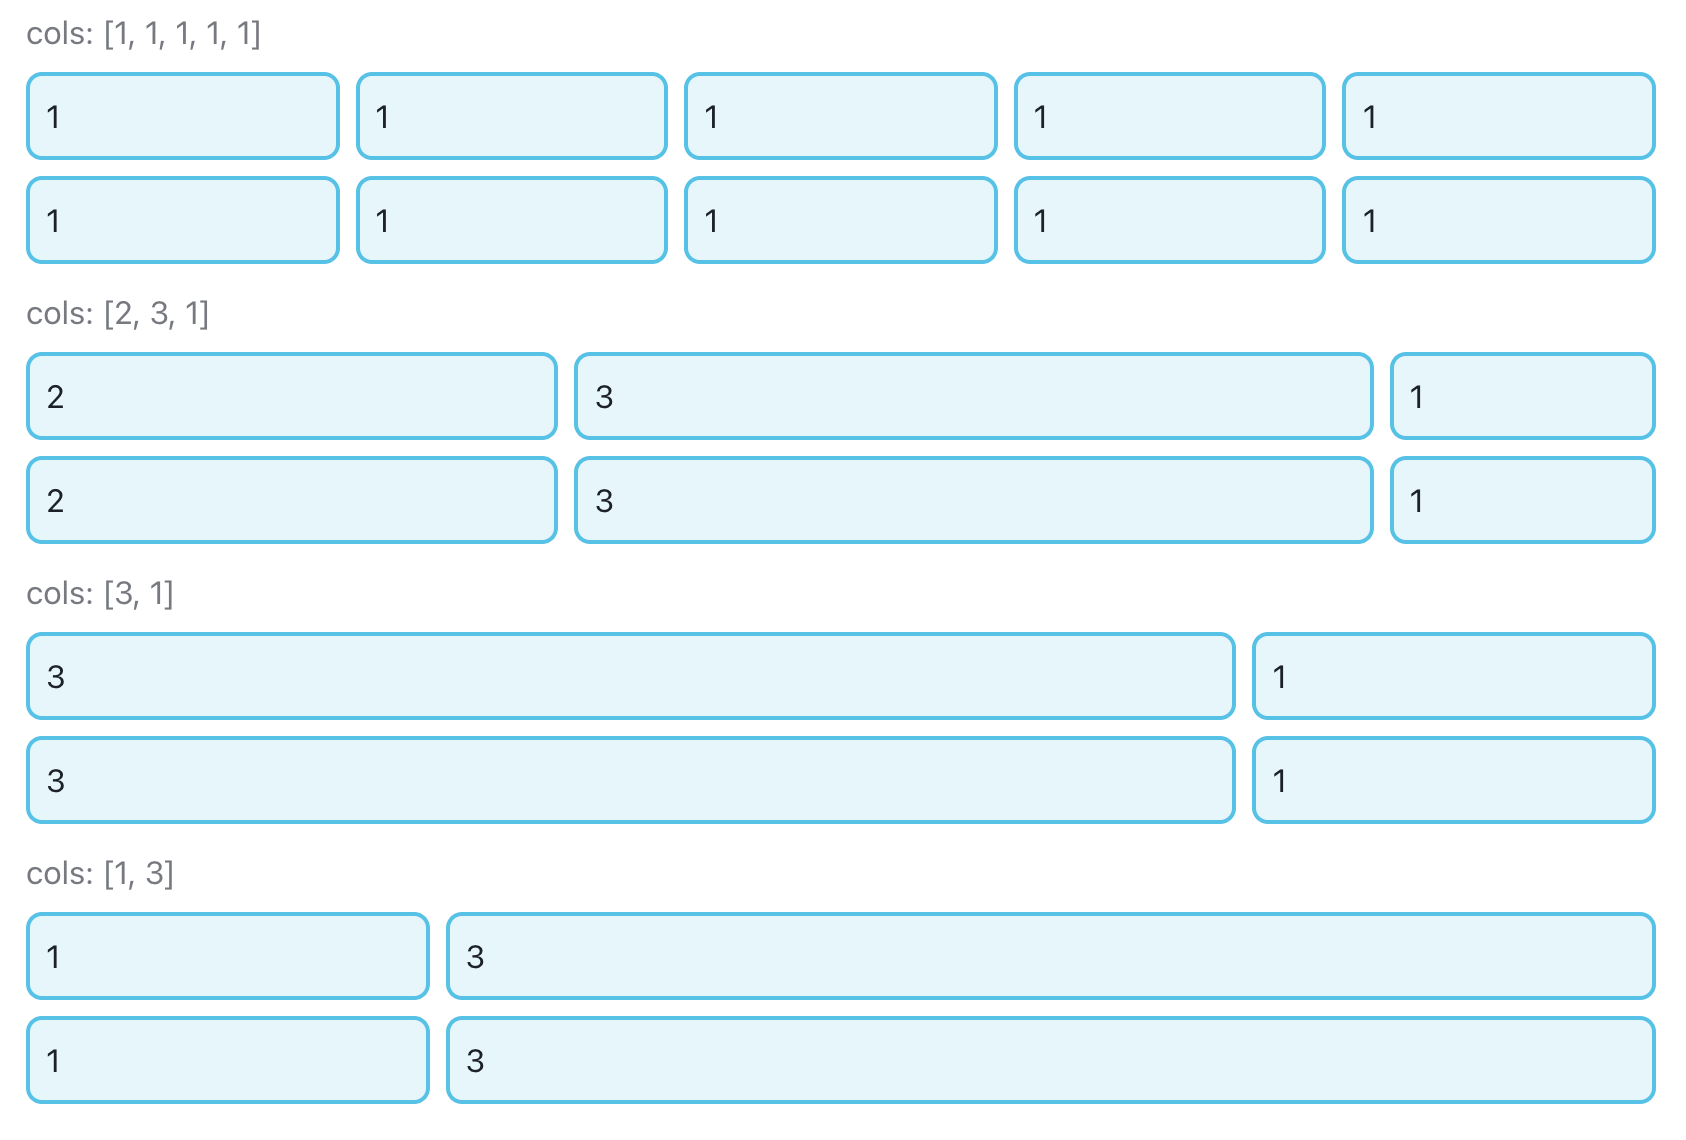
\includegraphics[width=13cm]{thesis/paper/images/grid.png}
  \caption{Grid component}%
  \label{fig:grid}%
\end{figure}

\subsection{Typography}

There are multiple components for typography, most of which are based off of the \texttt{text} component. All components for typography stems from the \texttt{text} component, but for ease of use, we defined aliases that utilises the \texttt{text} component with a set configuration. The properties that the \texttt{text} component accepts are \texttt{p}, \texttt{h1}, \texttt{h2}, \texttt{h3}, \texttt{b}, \texttt{i}, \texttt{u}, \texttt{block}, \texttt{muted}, \texttt{code} and \texttt{intent}. \texttt{p} stands for paragraph, which is used to define a paragraph block. \texttt{h1}, \texttt{h2}, \texttt{h3} represents headings, and their respective number represents the heading level. The behaviour is similar to HTML. \texttt{b}, \texttt{i}, \texttt{u} are styling options, represents bold, italics and underlined respectively. \texttt{muted} renders the text with a muted colour, useful for descriptions, subtexts or any secondary text that needs to be less attention grabbing. \texttt{code} renders the text with a light background and with monospace font family, should be used with codes. 

By default, the \texttt{text} component renders inline, meaning, the render output of \texttt{<text>1</text><text>2</text>} will appear side by side, as \texttt{12}. However, this behaviour changes for block-level properties; \texttt{p}, \texttt{h1}, \texttt{h2} and \texttt{h3}. \texttt{text} components that has these properties will take up the full line, and any other text component before or after them will fall into a new line. \texttt{block} property is a way to prevent text from rendering inline, without giving it any particular style. Text component also accepts \texttt{intent} property, which renders the text with the a colour given its intent. Last but not least, the text component can accept all layout properties just like any other component. The aliases that can be used in place of \texttt{text} are \texttt{p}, \texttt{h1}, \texttt{h2} and \texttt{h3} which will render a \texttt{text} component with the respective styles applied. All properties that the text component accepts can be used together to combine styles. For instance, a configuration such as \texttt{intent="error", b="true", u="true", h2="true" muted="true"} will result as a red h2 tag, muted, that is bold and underlined.

\subsection{Literals}

Literals are standalone string (or number) values provided to components (other than the \texttt{text} component) as children. Figure \ref{fig:text_vs_literal} shows the difference between a literal and a text value. While literals are not exactly a component themselves, they are nonetheless values that rendering needs to be handled by each client, thus they need their own renderer. The way literals are handled differs from platform to platform. For instance on the web client they can be rendered as is, while on other platforms they might need to be wrapped within special renderers where the native platform cannot handle them.

\begin{figure}
\begin{minipage}{\linewidth}
\begin{lstlisting}[language=xml]
<text>Handled by text renderer</text>
<block><text>Handled by text renderer</text></block>
<block>Handled by literal renderer</block>
\end{lstlisting}
\end{minipage}
\caption{Difference between text and literal nodes}%
\label{fig:text_vs_literal}%
\end{figure}

\subsection{Collapse}

The Collapse component can be used to hide long-form content within a collapse panel that is closed by default, and can be toggled open by clicking the handle. It accepts the complex attribute \texttt{handle} that takes the contents of the collapse handle. Its children will be rendered inside of the collapse. Collapse components can be nested, in which case each collapse component will operate individually. Figure \ref{fig:collapse_xml} shows how it can be used, and Figure \ref{fig:collapse} shows the render output of a collapse component on the Intertext web client.

\begin{figure}
\begin{minipage}{\linewidth}
\begin{lstlisting}[language=xml]
<collapse>
  <collapse.handle>
    <text>This is the handle</text>
  </collapse.handle>
  <text>This is the content</text>
</collapse>
\end{lstlisting}
\end{minipage}
\caption{How grid component is used}%
\label{fig:collapse_xml}%
\end{figure}

\begin{figure}
  \centering
  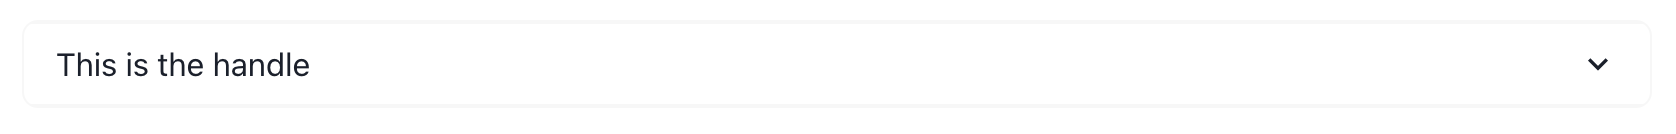
\includegraphics[width=13cm]{thesis/paper/images/collapse_closed.png}
  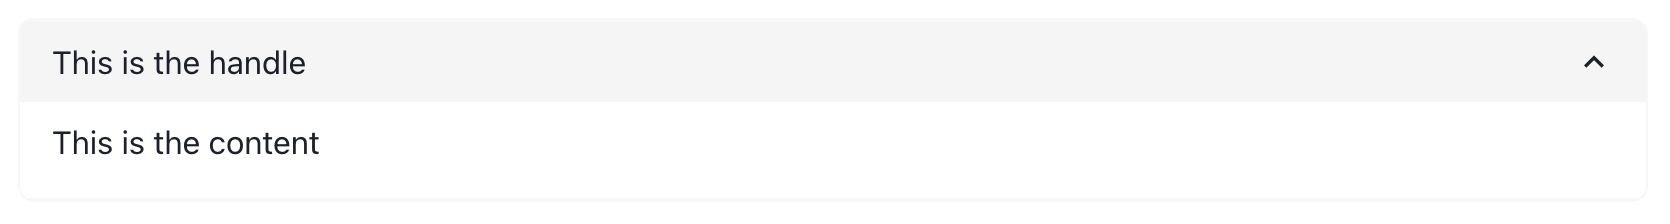
\includegraphics[width=13cm]{thesis/paper/images/collapse_open.png}
  \caption{Collapse component opened and closed state}%
  \label{fig:collapse}%
\end{figure}

\subsection{Button}

The Button component is simplest and the most primitive way of triggering commands. It accepts the \texttt{onClick} complex attribute, which can accept one or many commands under it.

\subsection{Input}

The Input component can be used to take text based input from the user. The type of the input can also be determined for validation purposes using the \texttt{type} attribute, with the accepted values at the time of writing being \texttt{text} (default), \texttt{email} and \texttt{password}. Input components are required to take \texttt{name} attribute, and a unique key to identify the input field should be provided. Intertext client automatically syncs the value of the input component to the state variable \texttt{inputState}, which gets passed on to the backend on every request within the request body. Lastly, input component accepts text as children to pre-populate its value.

\subsection{Image}

This command can be used to display images on the screen, for platforms that can support displaying images. It takes \texttt{src} attribute to accept the image URI, and a textual identifier for the image as \texttt{alt} attribute to display for platforms that cannot support images, such as the Intertext command-line client. At the time of the writing, the only acceptable way to display images in Intertext clients is to serve the images from the same origin. This is a result of the same origin policy as our privacy requirements. So for instance if IUIDL codes are being served from \texttt{example.com} and the \texttt{src} attribute is provided as \texttt{/assets/image.png}, Intertext client will try to load the image from \texttt{example.com/assets/image.png}. We have future plans of allowing assets to be loaded from remote servers after permission is granted by the user, which is explained in the \nameref{futureWork} section.

\section{Commands}

Similar to the components, commands also are registered to the engine. However the registration of the commands are more dynamic compared to the components; while components are static and are immediately available right after the initialisation, some commands rely on other artefacts to be available before they are able to be registered. For instance on the web client, the commands related to the client state requires the root component to be mounted, therefore they can only be registered after the mounting occurs. These requirements changes from client to client based on the platform requirements.

\subsection{State}

The State command is used to set the state or retrieve read a value from the state. This command is expected to be registered to the engine by each Intertext client based on how the state is handled on the host platform. For instance, for the web client, the client state is controlled by the root React component, therefore it can only be initialised once the component is initialised and mounted on screen. 

The State command accepts \texttt{key} attribute, which takes the key of the state variable. The children of the state command takes the value of the state to be set. Unlike other commands, state command can also be used as a component to display state values on the screen. When the state command is used without providing a value, the Intertext engine reads the state value, and interprets it as a literal value, uses the \texttt{literalRenderer} to display it on the screen. Additionally it takes the attribute \texttt{clear} to clear the state value. When this attribute is provided, Intertext client will clear the value instead of printing it even when no children is provided. Last but not least, a state command takes the attribute \texttt{persist} to target the persisted storage instead of the volatile storage. All attributes work the exact same way when \texttt{persist} attribute is provided, only difference being that it runs against the persisted storage. Figure \ref{fig:how_state_is_set_and_read} shows the syntax of how setting and reading the state works.

\begin{figure}[htb]
\begin{minipage}{\linewidth}
\begin{lstlisting}[language=xml]
<!-- set the `name` state value -->
<state key="name">John</state>

<!-- set the `name` state value to persisted storage -->
<state key="name" persist="true">John</state>

<!-- read and print the `name` value -->
<state key="name"></state>

<!-- read and  print the `name` value from the persisted storage -->
<state key="name" persist="true"></state>

<!-- clear the `name` value -->
<state key="name" clear="true"></state>

<!-- clear the `name` value from persisted storage -->
<state key="name" clear="true" persist="true"></state>
\end{lstlisting}

\end{minipage}
\caption{Example usage of the \texttt{state} command}%
\label{fig:how_state_is_set_and_read}%
\end{figure}

\subsection{Alert}

The Alert component is used to display a simple text-based message to the user. It uses the \texttt{<alert>}, and accepts the message as its children. An example usage can be seen in Figure \ref{fig:alert_command_usage}.

\begin{figure}[htb]
\begin{minipage}{\linewidth}
\begin{lstlisting}[language=xml]
<button>
  <text>Save</text>
  <button.onClick>
    <alert>Saved!</alert>
  </button.onClick>
</button>
\end{lstlisting}
\end{minipage}
\caption{Example of the \texttt{alert} command}%
\label{fig:alert_command_usage}%
\end{figure}

\subsection{OnLoad}

The \texttt{onload} command can be used to execute certain commands on page load. The concept of \dquote{page being loaded} differs from platform to platform, therefore each Intertext client is expected to implement this based on the platform requirements. For instance, the \dquote{load} event for the web client fires when the root React component is mounted on the screen. It takes no arguments, and takes one or more commands as its children. This command is especially useful for cases when a command needs to be executed straight away without waiting for user interaction, for things such as setting the state or making a request. An example usage of \texttt{onload} is shown in Figure \ref{fig:onload_usage}.

\begin{figure}[htb]
\begin{minipage}{\linewidth}
\begin{lstlisting}[language=xml]
<onload>
  <alert>Page loaded!</alert>
</onload>
\end{lstlisting}
\end{minipage}
\caption{Example of the \texttt{onload} command}%
\label{fig:onload_usage}%
\end{figure}

\subsection{Timeout}

The \texttt{timeout} command takes other commands as its children, and executes them with a given delay. The delay can be provided using the \texttt{delay} attribute in milliseconds. An example usage of \texttt{timeout} is shown in Figure \ref{fig:timeout_usage} to demonstrate how a simple \dquote{polling} mechanism can be implemented by combining \texttt{timeout} and \texttt{onload} commands.

\begin{figure}[htb]
\begin{minipage}{\linewidth}
\begin{lstlisting}[language=xml]
<!-- /poll: if task is not finished -->
<onload>
  <timeout delay="5000">
    <request endpoint="/poll"></request>
  </timeout>
</onload>
\end{lstlisting}
\begin{lstlisting}[language=xml]
<!-- /poll: if task is finished -->
<onload>
  <alert>
    Task completed!
  </alert>
</onload>
\end{lstlisting}
\end{minipage}
\caption{Example of the \texttt{timeout} command}%
\label{fig:timeout_usage}%
\end{figure}

\subsection{Request}

The \texttt{request} command is a general purpose command that can be used to instruct Intertext client to make a request to the server. It takes \texttt{endpoint} attribute, which can be used to provide which endpoint should the request target. For this attribute, an endpoint relative to the origin must be provided, as per our privacy requirements, we implement a same origin policy where Intertext clients will only make requests on behalf of an origin to the same origin itself. So if IUIDL is being served from \texttt{example.com}, the \texttt{endpoint} attribute provided must look like \texttt{/some/path}, in which case the Intertext client will make the request to \texttt{example.com/some/path}. As explained further in \nameref{futureWork} section, we plan to implement a permission flow that when an origin tries to make a request to another origin, Intertext client would ask the user, and only make the request when permission is granted.

All requests made to the backend are \texttt{POST} requests, in order to attach the overhead to each request body. With each request, Intertext client passes \texttt{state}, \texttt{persist} and \texttt{inputState} values; which are the volatile state, persisted state and the state of the input fields on the current page respectively. On the server side, these values can be used to build custom logic.

With every request, the backend endpoint is expected to return some IUIDL code. The \texttt{request} command accepts the attribute \texttt{strategy} to specify what Intertext client should do with the IUIDL code server responds with. There are 5 strategies that can be passed; \texttt{replace}, \texttt{append}, \texttt{prepend}, \texttt{execute} and \texttt{ignore}. The \texttt{replace} option is the default option, and it simply replaces the entire page contents with the IUIDL code that are received. \texttt{append} and \texttt{prepend} as the name suggests appends and prepends the IUIDL code respectively to the existing packages on the screen. These strategies could be useful for implementing functions such as \dquote{load more}. \texttt{execute} strategy does not tamper with the existing page contents, however parses the received IUIDL code and tries to execute it as if they are commands, and the packages that are not commands gets ignored. This strategy can be used with the \texttt{onload} command for when the response of an endpoint is expected to be of type command. The \texttt{ignore} strategy completely ignores the response. It should be used only when the server-side needs to be notified of an event.

\subsection{Navigate}

This command by nature is exactly the same as the \texttt{request} command. It accepts an \texttt{endpoint} argument, and makes an identical request as the \texttt{request} command makes to that endpoint. The reason why it is separated from \texttt{request} and made into its own command is to let the Intertext client know that the purpose of this request is to have user transition from one screen to another. This command does not accept the \texttt{strategy} attribute, and uses the \texttt{replace} strategy by default. Moreover, the Intertext client identifies this transition as a navigation and makes certain arrangements which is specific to the host platform. For instance, Intertext web client keeps Intertext address bars state, browser address bars state, and browsers history state in sync with the current page. This assures native browser features such as forward/back button to function with the Intertext app. When \texttt{navigation} command is used to transition from one screen to another, the client updates the two address bar states, and pushes the new state to the browsers history stack. Therefore, this command should only be used to transition between pages.

% !TEX root = ../thesis.tex

\chapter{Use Cases and Evaluation} \label{evaluation}

In this section, we will first walk through some example use cases for Intertext. It is worth noting that at the time of writing, only the Intertext web client is fully implemented. Therefore some of the examples mentioned in this section are given with our future plans in mind. Moreover, some of the use cases are of things that could theoretically and practically be built on top of the Intertext ecosystem, not by us but by the community. 

Later on, we will explain the evaluation process. To execute the evaluation, we have built \dquote{RecipeApp}, a sample Intertext application where users can sign up, log in, add recipes, and browse recipes other users added. It was specifically built to showcase all the functionality that Intertext offers. While the use cases section is intended as example use cases for the users, this section could be thought of an example use case scenario for developers, giving ideas on how an Intertext application can be built. In this section, we will first talk about RecipeApp; how it's built and how it works under the hood. Then, we will discuss the user evaluation process and share the results.

\section{Use Cases}

\subsection{Back-end Developer}

Harry is a software engineer. He recently graduated from college, and started his career as a backend engineer. While work is busy, he is still interested in working on an idea he had in college on the side. Without losing much time, he gets to work. His most important constraint is that he has little to no budget, so he designs a low-cost scaleable serverless architecture and starts coding. After a few months of hard work, he finishes the backend portion of his application. He spins up an instance on his favourite cloud provider, he is able to utilise the generous free-tier and the free credits offered by the provider to scale up to thousands if not millions of users at almost no cost. 

Then he realises that he still needs a front-end for his application. Not only he needs a web presence, he also needs a mobile app to meet his users needs. He has no front-end experience, nor does he have the budget to outsource the task or time to learn. So he decides to make his product an Intertext application. He makes use of the existing backend to create an additional endpoint that serves the front-end in IUIDL, and in a matter of days, he finishes the fully functional front-end and is ready for the beta launch. With minimal effort, he was not only able to obtain web and mobile presence, his product supported all other Intertext clients as well.

\subsection{John's Old Parents}

John regularly visits his old parents. A few visits back, he brought with him a gift, a computer, as an effort to introduce them to technology. He helped set it up, and gave them a walk through on how to use it. He thought them how to perform tasks such as online banking, checking the news, checking the weather, using social media and so on. 

On his last visit, his parents mentions that they were having some problems with the computer. He turns it on to assist them, only to find that the computer is filled with of harmful malware and games/apps that were clearly downloaded out of intention. He asks them how it happened, and they told him that it all started when they clicked "OK" on a popup that appeared on one of the websites. The default home page was replaced, new harmful browser extensions were installed, the computer became slow and was nearly unusable. So he formats the computer, and installs the Intertext desktop client. He teaches them about how to use the Intertext apps for their favourite news websites, bank, social media, and other services they use. He tells them that they can enjoy a clean, consistent and safe experience, with no intrusive ads, harmful software, trackers, background scripts and so on. 

Another thing that he notices is that they struggle to see the screen and read text very well. Also since they aren't accustomed to using a computer mouse, their mouse movement is unstable and clicks are inaccurate. They often misclick on things they did not intent to click, causing them to navigate away to another page and miss context, which gets them confused and frustrated. To combat these issues, he creates a custom theme for them. He makes the text bigger and bolder, buttons and links larger and harder to miss. Thanks to Intertext, his parents are able to use web more comfortably and confidently.

\subsection{New Device On The Market}

X, Inc is a promising startup working on a new kind of wearable device. This device can perform all functions of a mobile phone; make calls, send messages, take pictures, browse the internet and so on. It has the potential to replace mobile devices for some people, however it has a downside that holds it back: it has no application support. There are no third party applications built that can run on their device natively. It do have a web browser; but due to the nature of this device, browsing web applications on its screen is very uncomfortable. They realise that their potential customers don't want to leave their phone behind when they can't use their day-to-day applications properly. As a solution, they decide to make use of the open-source Intertext ecosystem. They build an Intertext client that runs natively on their device and renders IUIDL optimised for its input/output (I/O) constraints. With their new Intertext client, they now have access to the entirety of the Intertext applications. They are now set to release their product with no compromises and full confidence.

\subsection{Clients For Special Needs}

Sally is a developer working on an initiative for creating software that makes it possible for people with disabilities that cannot use a mouse or a keyboard to be able to use a computer. They experiment with different input/output methods such as retina tracking, voice interfaces, neural-control interfaces and so on. With their software, users can chose the I/O method that best suits them to use their computer. However in most cases, it is very hard to use a software that was built with no accessibility features. So she decides to use Intertext to improve this process. Knowing that it is guaranteed that all Intertext applications are accessible by default, she builds the software to take advantage of the Intertext web client. Moreover, for other I/O methods they experiment with that needs support for a custom/specific GUI, she creates individual Intertext applications.

\subsection{No-Code Universal Application Builder}

With the increasing popularity of the no-code movement, more and more companies are looking for code-free solutions to problems that used to require programming skills. Y, Inc is one of these companies. They want to invest in a platform that allows everyone to create applications for different devices and environments. They are also aware of their constraints. They know that a one-size-fits-all solution is extremely hard to build, as every platform runs on different technologies, they have different layout systems, different runtime and so on. And then they discover Intertext. They realise how easy it is to create a tool to build Intertext applications, since all there is to do is to generate simple IUIDL code in XML syntax. Also, the logic that front-end applications needs to perform such as making requests and state management are also operated through the same syntax. Moreover, the applications generated by the tool would be universal, that is, it could run on every platform that Intertext has a client for and will have a client for in the future. They create a service that allows users to build and serve Intertext applications with ease, without writing a single line of code. This makes it possible for hobbyists to put together a simple interface without prior programming knowledge.

 
\section{RecipeApp}

While building RecipeApp, we wanted to keep things simple as its purpose is demonstration of Intertext, and we still tried our best to stay true to a real wold scenario of building applications. We created a real backend application that serves IUIDL through a restful endpoint. We used Node.js as the server-side technology, and express framework to create the endpoints. As for the database, we created a fake api that resembles a real Object-relation Mapping (ORM), which stores data in the memory.

In a real-world front-end application, it is very common to create UI elements as reusable components. This is no different for Intertext application, in a real world scenario it is clear that the best practice would be to create components out of commonly repeating UI patterns, and use instances of those components rather than duplicating IUIDL code. While creating components and reusing them on the front-end is much simpler as there are many front-end frameworks/libraries like React that enables building UI declaratively and eliminates the need for imperative manipulations, in order to do this with ease on the backend side, we needed a templating engine. For this purposes, we used the Handlebars, a popular template engine for Node.js applications.

For the time being, only the web client of Intertext is fully implemented. Therefore, the demonstration will be made on the web client and all respective screenshots are from there. However once the other clients are ready, they will be able consume the same application as it is.

\subsection{Introduction}

\begin{figure}[htb]
  \centering
  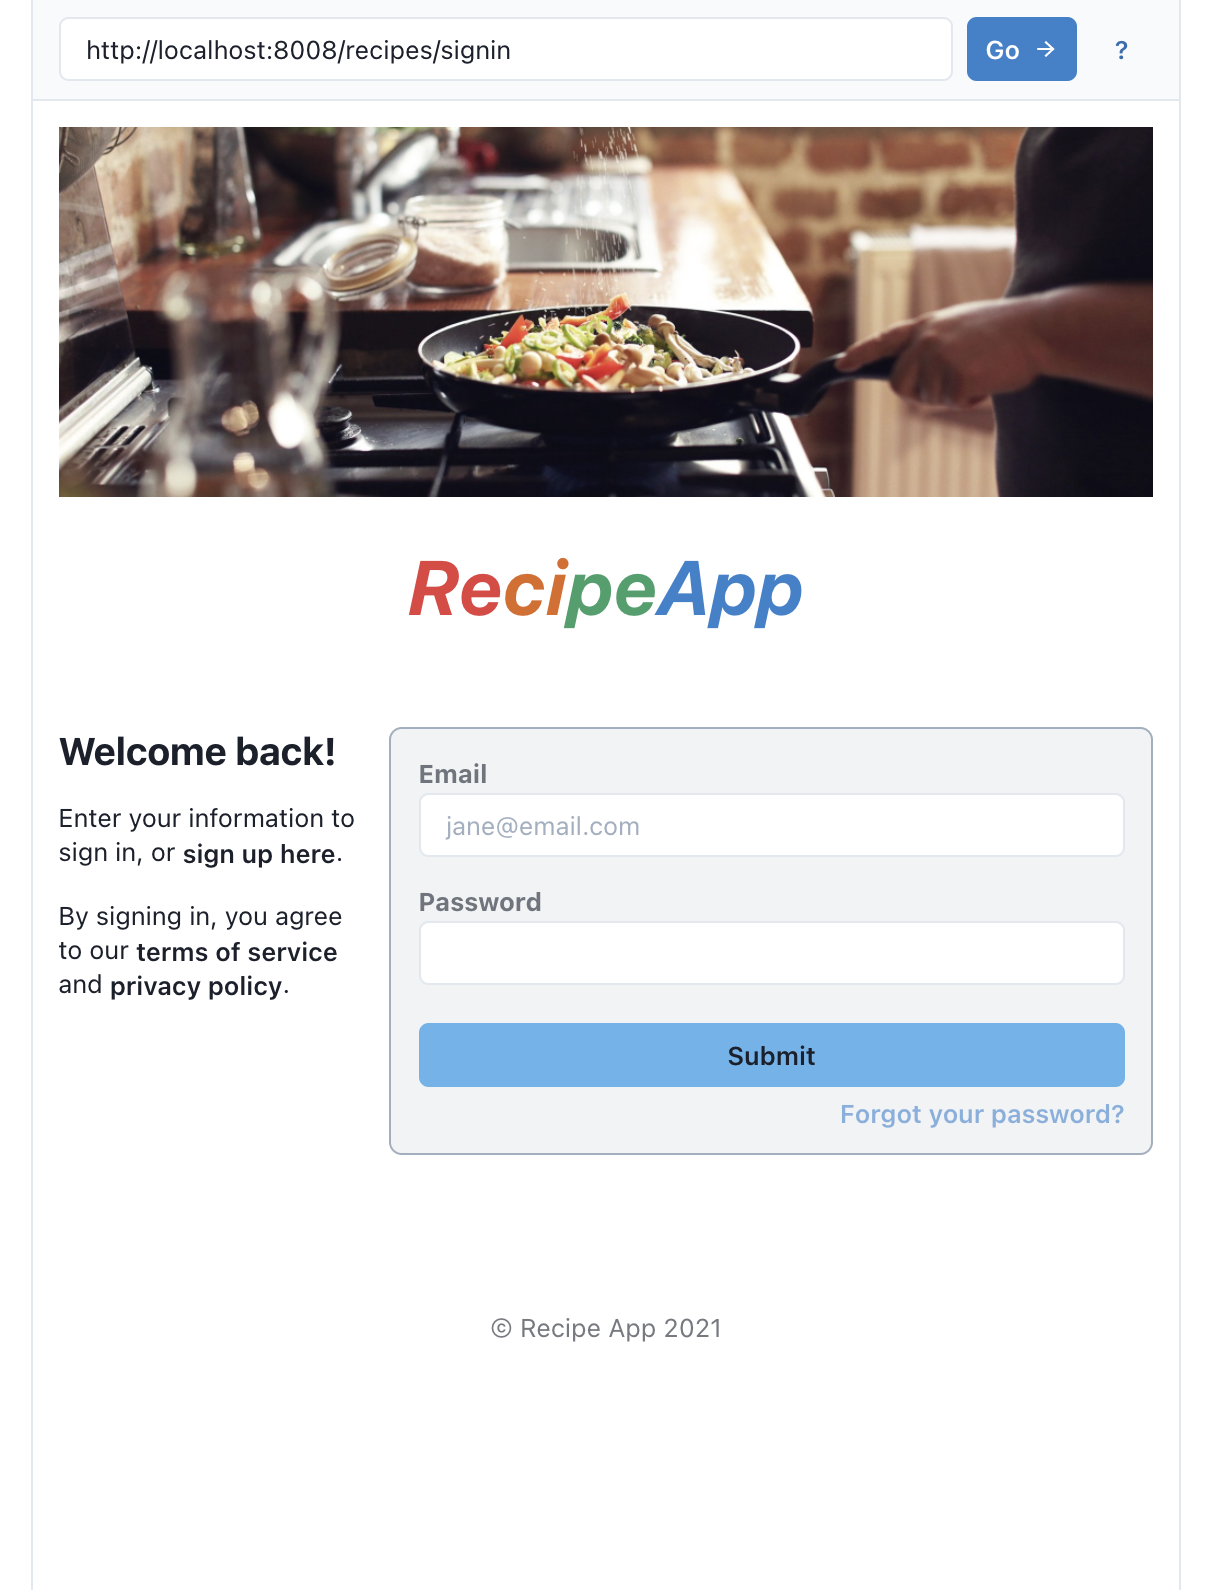
\includegraphics[width=6.2cm]{thesis/paper/images/rec_signin.png}
  \,
  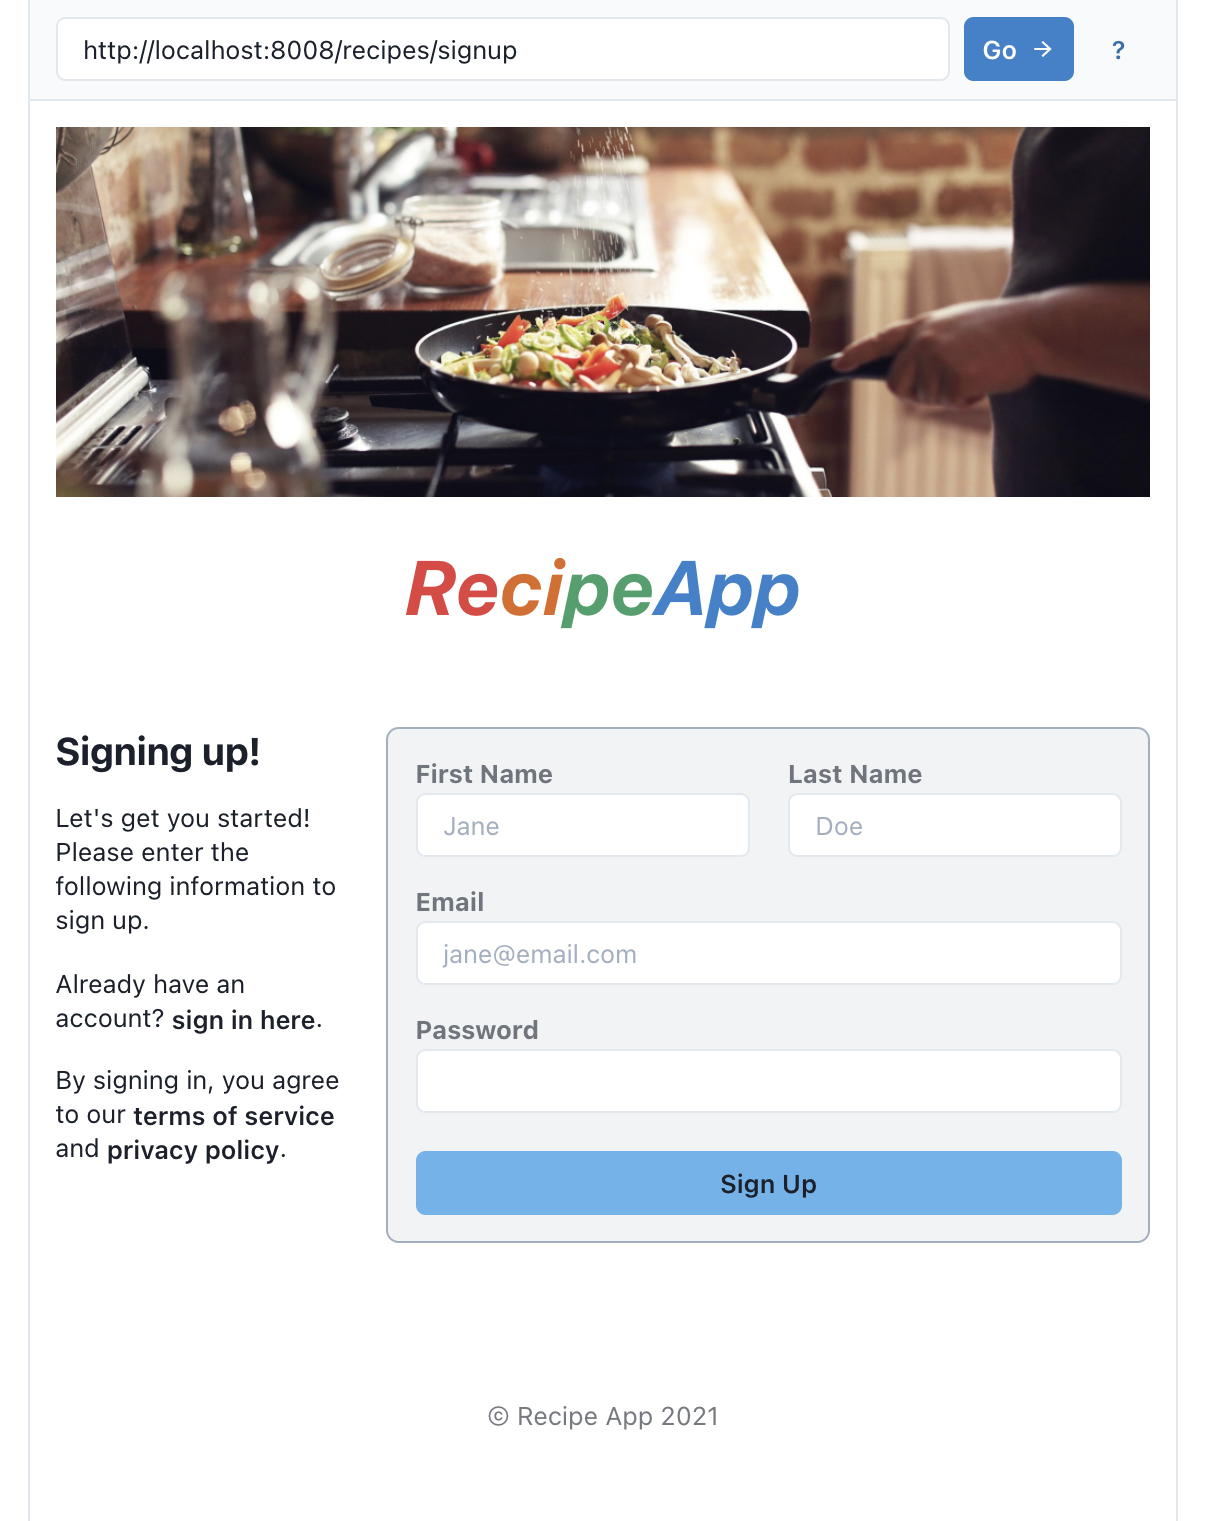
\includegraphics[width=6.2cm]{thesis/paper/images/res_signup.png}
  \caption{RecipeApp Sign In/Sign Up screens}%
  \label{fig:rec_signin_signup}%
\end{figure}

First, user visits the URL the RecipeApp is served from via the address bar above. In figure \ref{fig:rec_signin_signup} the example server runs on \texttt{http://localhost:3000} and the endpoint RecipeApp is served from is \texttt{/recipes}. If user is not already signed in, they will be redirected to \texttt{/recipes/signin}. After signing in from this screen, they will be redirected back to the application. If they were visiting a particular URL such as \texttt{/recipes/new} or \texttt{/recipes/3} before they got redirected to the sign in screen, they will be redirected back to that screen after signing in. Once they are signed in, they will be presented with the recipe list. Recipe list has two view options, grid view and list view, which user can chose between. The view selection will persist across sessions. Moreover, the list features a search bar, which can be used to search recipes by keywords. On each recipe item, there difficulty and time it takes to prepare the recipe is displayed along with an image. From the top navigation, user can click on the Add Recipe button to go to the insert page. From there, they can insert their own recipe.

\subsection{Authentication}

Before the authentication, first thing to understand is how we implemented the redirection system. The redirect screen, which can be seen in figure \ref{fig:rec_redirect}, is essentially an handlebars template that can be rendered with some parameters and can be used for different purposes. There are two essential functions of this screen; it instructs Intertext client to store some data, and to redirect user to another endpoint. The parameters changes based on the user case.

\begin{figure}[htb]
  \centering
  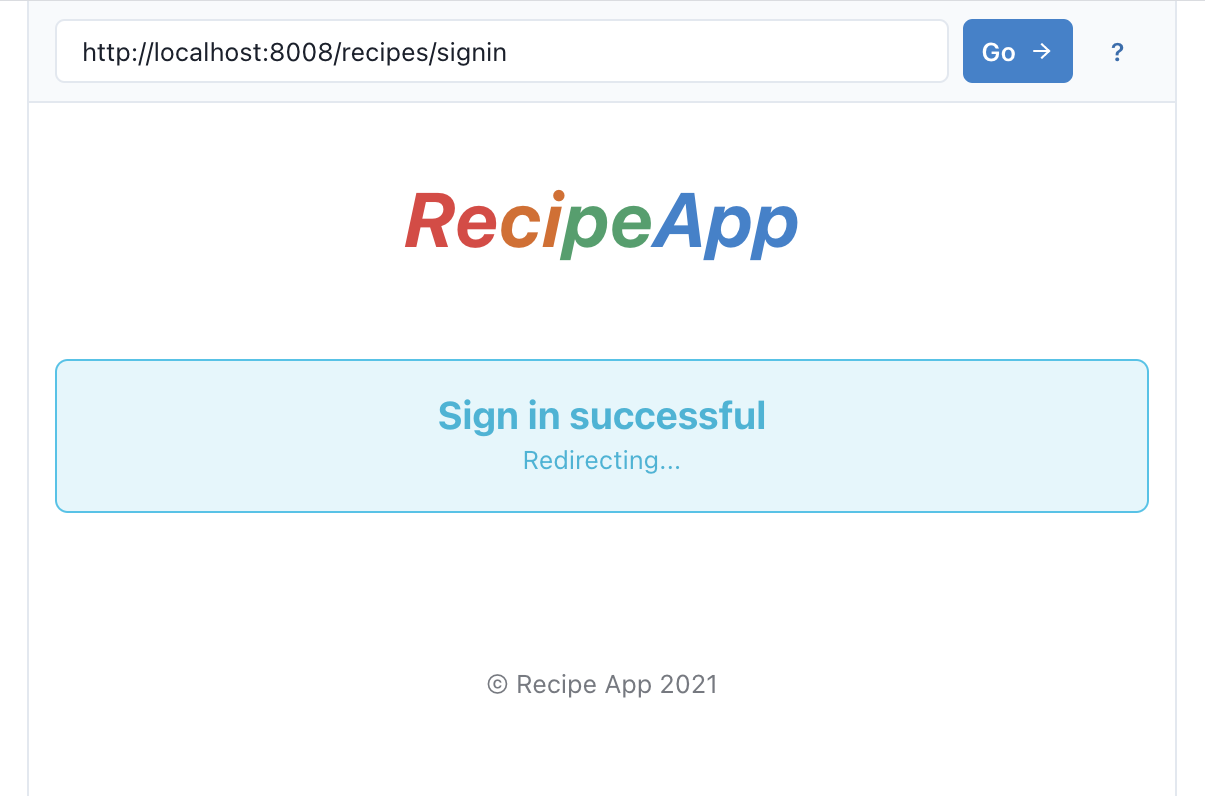
\includegraphics[width=12.4cm]{thesis/paper/images/rec_redirect.png}
  \caption{Redirect screen}%
  \label{fig:rec_redirect}%
\end{figure}

As we established before, Intertext clients passes on the application state along with every single request. When user visits the application URL, the server receives the persisted state, which is where the user token is expected to be if the user is logged in. When a user lands on any page of RecipeApp that is behind the authentication wall, the server checks the presence of \texttt{token} in request body, and if it is not present, it renders the redirect screen as shown in figure \nameref{fig:token_capture}. 

\begin{figure}[htb]
\begin{minipage}{\linewidth}
\begin{lstlisting}[language=javascript]
const token = get(req, "body.persist.token");
if (!token) {
  res.render(view("redirect"), { ... });
} else {
  res.render(view("home"), { ... });
}
\end{lstlisting}
\end{minipage}
\caption{How token is captured on the backend}%
\label{fig:token_capture}%
\end{figure}

The redirect screen does two things: it instructs the client to store a variable called \texttt{auth-callback} which holds the URL that user is at, and it instructs the Intertext client to navigate to the \texttt{/signin} endpoint. Intertext clients does these two things, and redirects user to the \texttt{/signin} endpoint, triggering another request to the backend. The \texttt{/signin} endpoint on the backend renders the sign in form. After user submits the form with their credentials, another request to the \texttt{/signin} endpoint is made, but this time with the credentials. Backend then checks the credentials, and if it is a successful login, it once again renders the redirect screen. The redirect screen again performs two tasks: first it instructs the Intertext client to store the \texttt{token} to the persisted storage. Then, if the \texttt{auth-callback} variable is present in the request body of the request made to the \texttt{/signin} endpoint (which is where the URL user was redirected to the sign in endpoint from is stored at), it instructs the Intertext client to redirect back to that endpoint, otherwise it redirects to the home screen.

\subsection{Recipe List}

The recipes view features a list of the recipes. As seen in in figure \ref{fig:rec_recipe_list}, it has several components: recipe title, description, difficulty and time to cook details that are displayed in tags, and a read more button to navigate to the recipe page. The difficulty tags are made of the \texttt{block} component, and they use intents to hint the difficulty of the recipe. The view has two display options, a list view and a grid view. It also has a search input to search recipes.

\begin{figure}[htb]
  \centering
  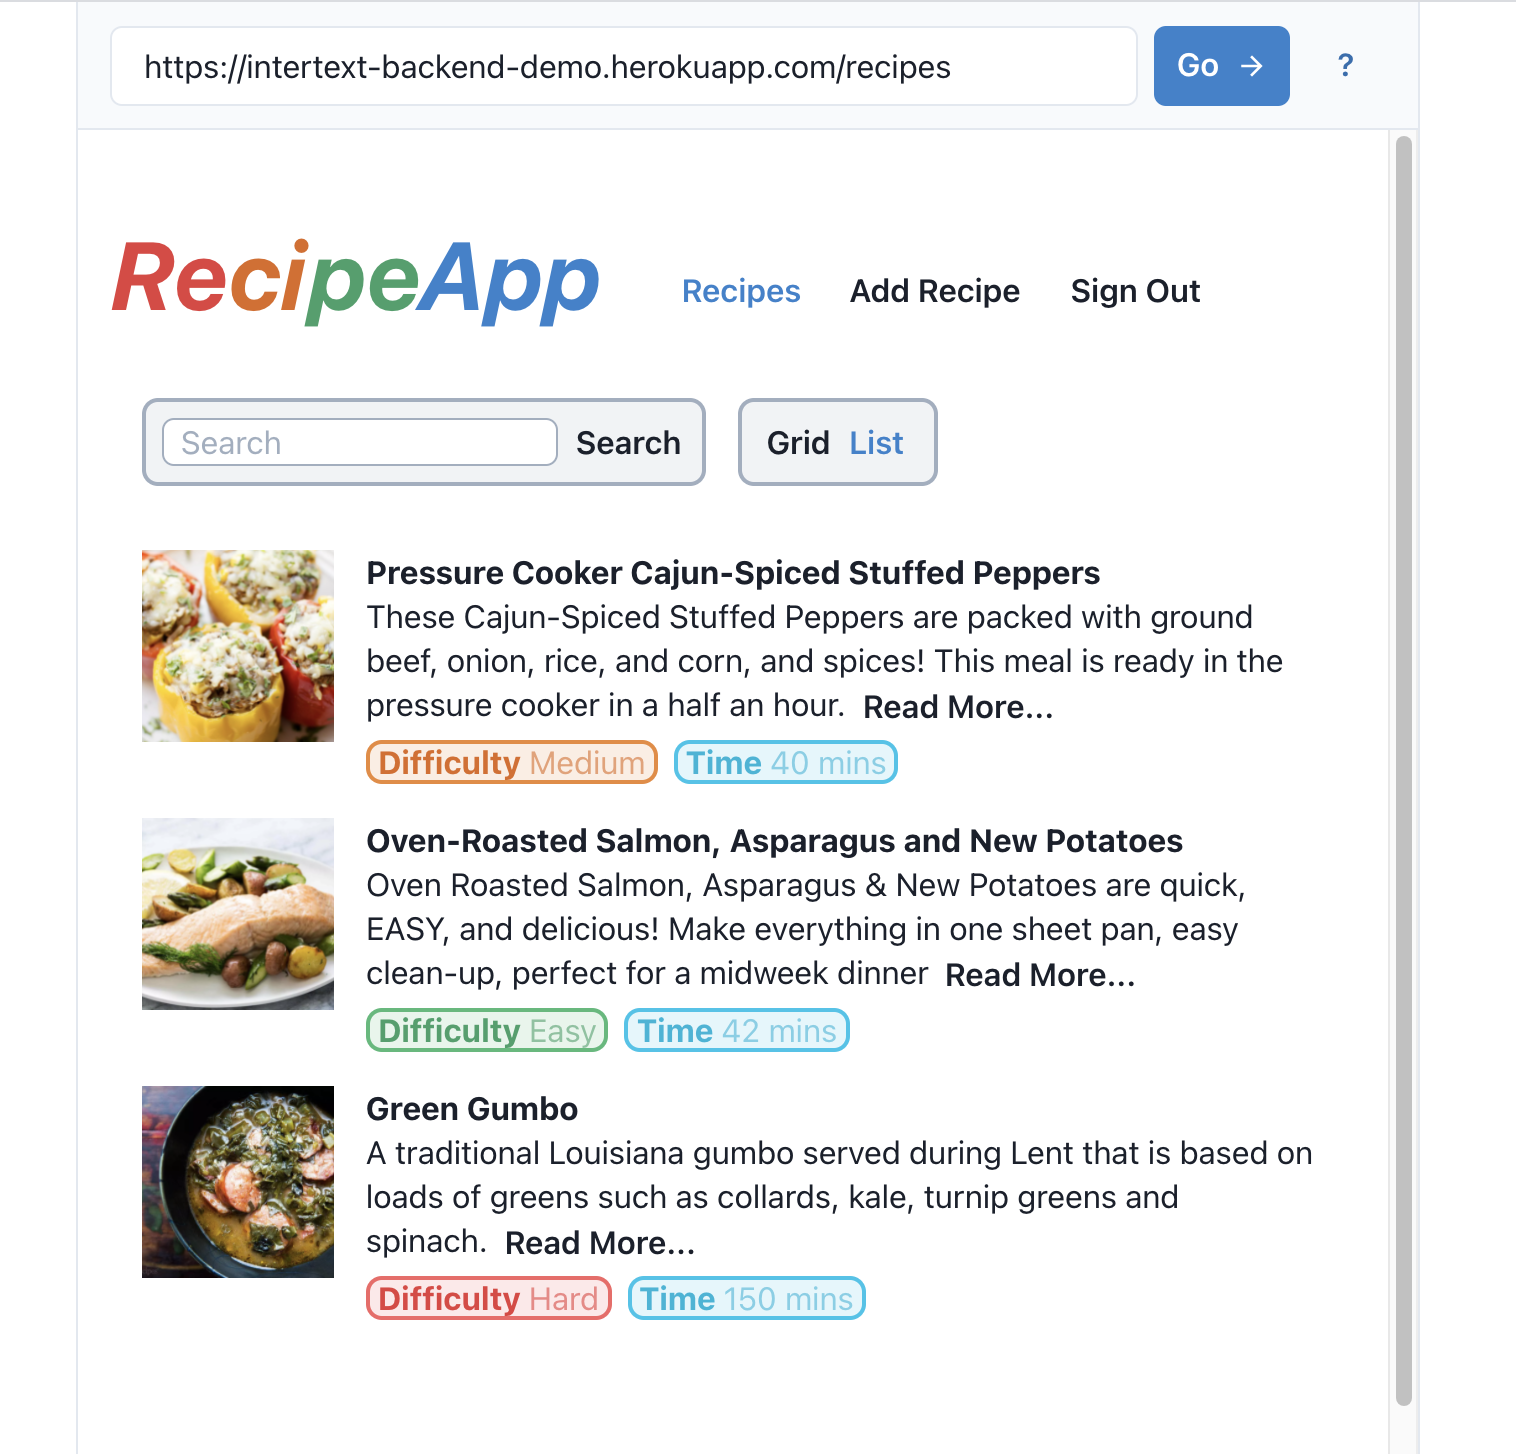
\includegraphics[width=6.2cm]{thesis/paper/images/recipe_list.png}
  \,
  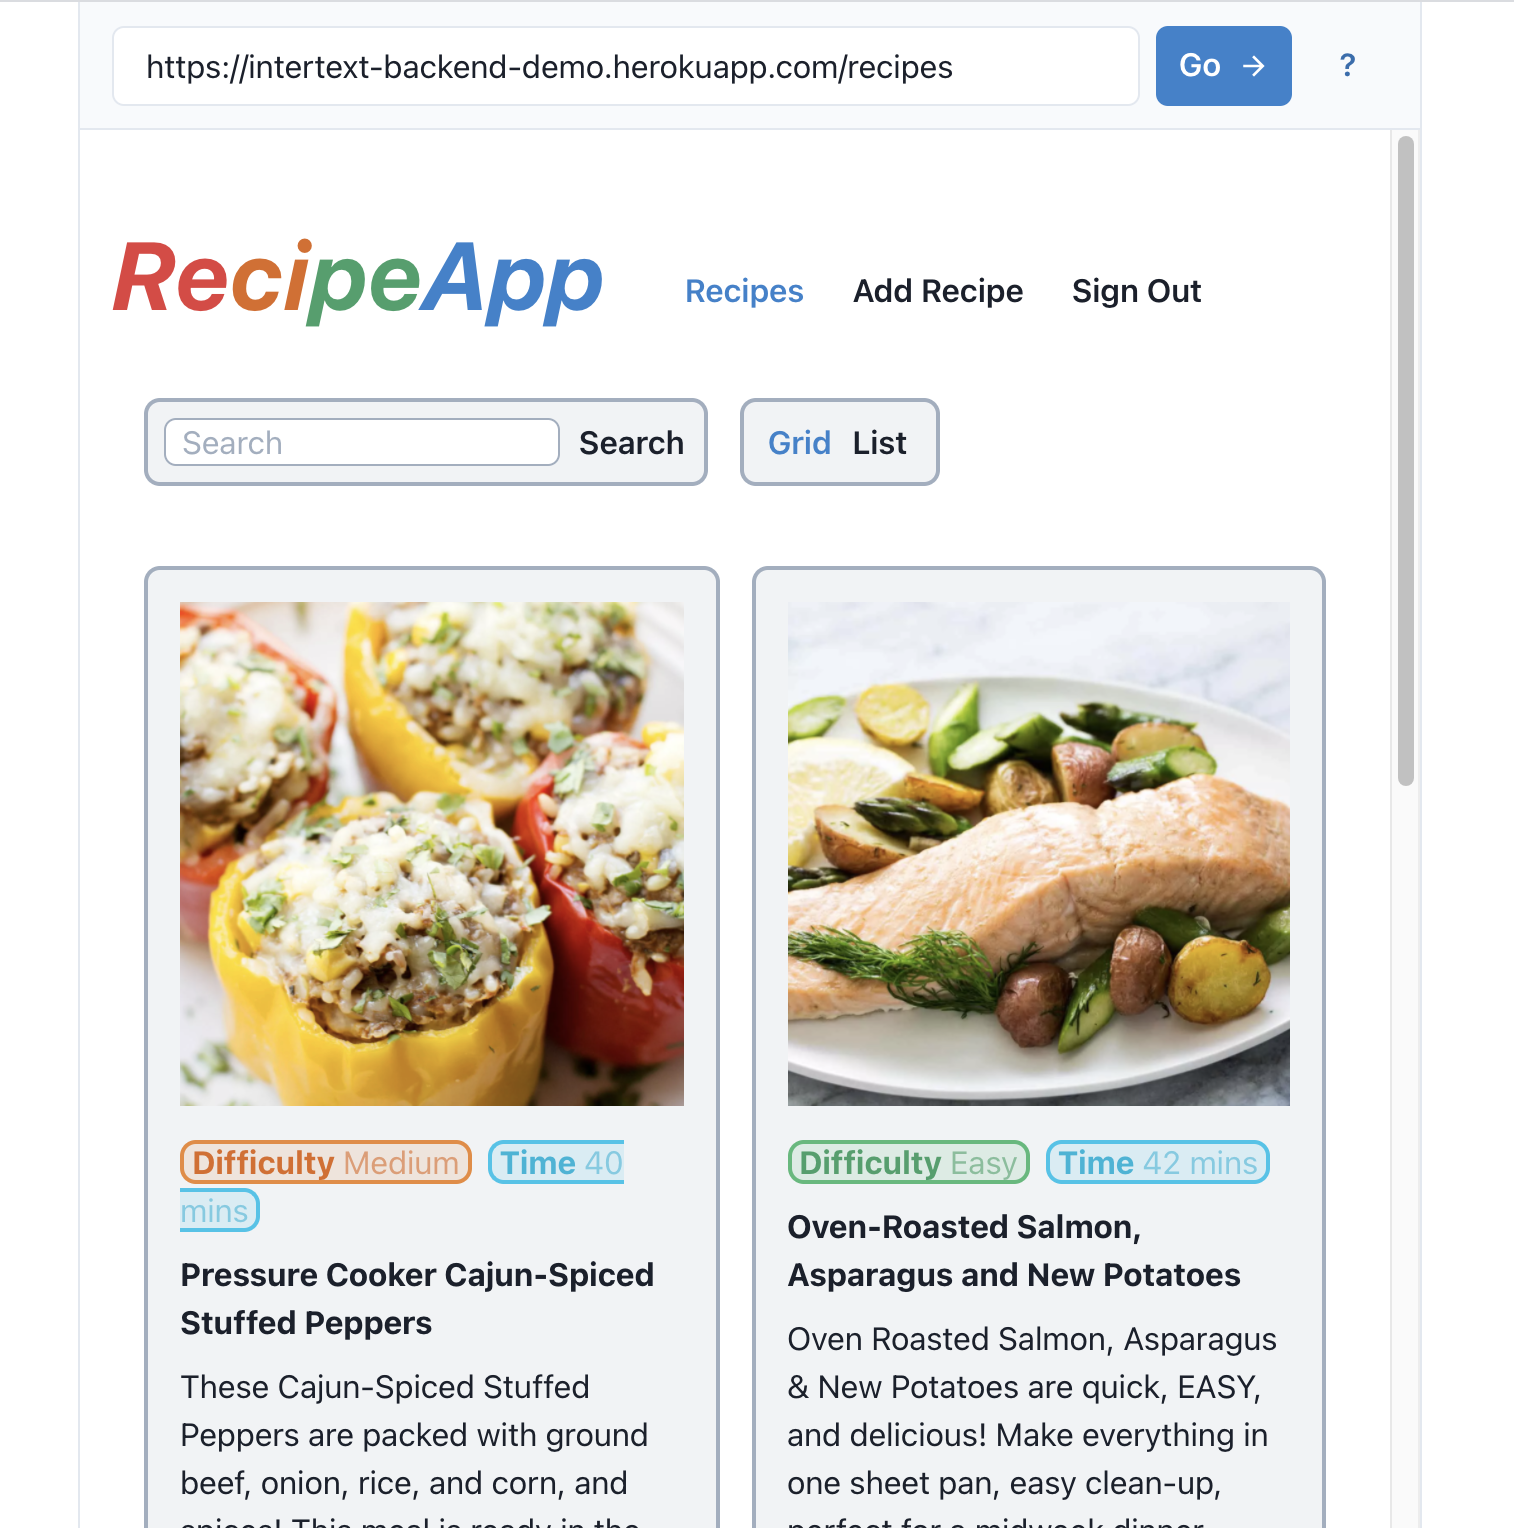
\includegraphics[width=6.2cm]{thesis/paper/images/recipe_grid.png}
  \caption{RecipeApp Recipe List Grid/List Views}%
  \label{fig:rec_recipe_list}%
\end{figure}

Both the input and display preference options work in the same way, by modifying the front-end state and triggering a request to the backend to pick up the modified state. As user types into the text input, Intertext client automatically saves its value into the state that gets passed on to the backend on every request. The "Search" button next to the search input only triggers a request to the \texttt{/recipes} endpoint. The recipes endpoint receives the query in the search input, and filters the results accordingly. It also pre-populates the input value by passing the query as a children to the \texttt{input} component. The display options on the other hand first sets the front-end state variable \texttt{layout} to either \texttt{grid} or \texttt{list}, and again triggers a request to the same \texttt{recipes} endpoint as seen in figure \ref{fig:rec_display_options}. The backend picks up the variable and renders the different version of the displays accordingly. The primary color of the button for the active display option is also controlled by the same \texttt{layout} variable, backend renders the buttons with the relevant intent based on that variable also as seen in figure \ref{fig:rec_display_options}.

\begin{figure}[htb]
\begin{minipage}{\linewidth}
\begin{lstlisting}[language=xml]
{{#> button_small}}
  <text intent="{{#if layout_grid}}primary{{else}}{{/if}}">Grid</text>
  <button.onClick>
    <state key="layout" persist="true">grid</state>
    <request endpoint="/recipes"></request>
  </button.onClick>
{{/button_small}}
{{#> button_small}}
  <text intent="{{#if layout_list}}primary{{else}}{{/if}}">List</text>
  <button.onClick>
    <state key="layout" persist="true">list</state>
    <request endpoint="/recipes"></request>
  </button.onClick>
{{/button_small}}
\end{lstlisting}
\end{minipage}
\caption{Redirect screen example}%
\label{fig:rec_display_options}%
\end{figure}


\section{Evaluation}

In this section, we explain how we conducted our user study for user evaluation. We first explain our methodology, and then share the results of our evaluation.

\subsection{Methodology}

We conducted our user study in the form of surveys. We used Google Forms to create the survey and manage the responses. In the surveys, we first gave some information and/or material to investigate, then followed it with likert scale questions.

We utilised Amazon's Mechanical Turk (MTurk) service in order to find participants. We stated the description and intentions of each survey on their respective survey page. Some of our surveys required special skills, for which we used features provided by MTurk that enables us to only target participants with special skills. We set the compensation price per answer to 10 cents for general participation surveys, and 50 cents for surveys that requires special skills. We required our participants to enter their \textit{worker id} both on the surveys and on the respective survey page on MTurk, so that we can match the responses of the participants with their MTurk profiles to verify only our intended audience has participated, and duplicate/third party responses are eliminated.

Our user evaluation was conducted in two stages. First stage was to validate the problems in our problem statement that we are intending to solve, and the second stage was to validate Intertext, the solution we offer in order to address these problems. 

\paragraph{Phase 1: Problem Validation}

Here we aimed to validate the problem we are intending to solve. We first asked some optional identifying questions to ask about the background of the participants; including their age, gender, country of origin and occupation. Then, we separated questions into groups for every main category in our \nameref{problemStatement} section. We directed this section only towards the end-users.

\paragraph{Phase 2: Solution Validation}

Our project targets two different user group; developers, and end-users. Developers will use Intertext technology to develop products and services, and their end-users will use applications made within the Intertext platform. Both developers and end-users have separate benefits. In this phase of the user evaluation, we targeted both developers and end-users. 

We created two separate surveys, one for developers and one for end-users. On the survey we prepared for the end-users, we first gave a brief explanation of what Intertext is and what it does without going into technical details. We told about Intertext clients, how it works and how it can be used. We kept it as simple as possible, to make sure the general public can understand it. We also linked to a demo from the Intertext web client. Then, similarly to what we did in the first phase, we stated every problem from the \nameref{problemStatement} section. For every problem, we wrote a short paragraph explaining what the problem exactly is, and one explaining how Intertext addresses that problem. Then, we followed it with likert scale questions. 

For the developer survey, we started it off by duplicating the one for end-users and removing the questions. We kept the information parts identical, as developers also needs to understand what Intertext does and why it is beneficial to the users. We then created an extra section to give a technical overview of how Intertext works, benefits, and how Intertext applications can be developed. We also included a link to the repository that hosts \texttt{RecipeApp}, our demo Intertext application. Next, we listed the developer-related problems from the \nameref{problemStatement} section, wrote a paragraph explaining it, and another paragraph explaining the solution. We followed it with likert scale questions just like in end-user survey format.

In our likert scale questions, we focused on the trade-offs in order to get answers as objective as possible. To elaborate on this, if we were to explained that we solved a problem, and then followed it with a question asking about the thoughts on the solution, the responses would most certainly be positive. Solving a problem often comes with a trade-off, and this trade-off might not be immediately visible to the participant. We attempted to ask questions in a way that raises an awareness about the trade-offs, and validates if participant is on board with the solution regardless of it. For example, one of the solutions we offer is guaranteed security by eliminating third-party code execution, and the trade-off of this is that the platform will not support rich front-end functionalities and experiences. For general public, this trade-off would likely be overlooked. Thus, the likert scale question we asked about this solution was \textit{I would prefer guaranteed privacy and security over rich front-end functionality}, validating that users care more about privacy and security than rich front-end functionality.

\subsection{Phase 1 Results}

In the first phase, we received 119 responses (after filtering out duplicate answers and answers with invalid worker ids). Our results for the first phase are very positive, we were able to validate the problem and implement Intertext with more confidence. First three graphs shows age distribution, gender and country of origin of the respondents, and the ones that follows shows the responses given to each question alongside the question text underneath.

\begin{figure}[H]
  \centering
  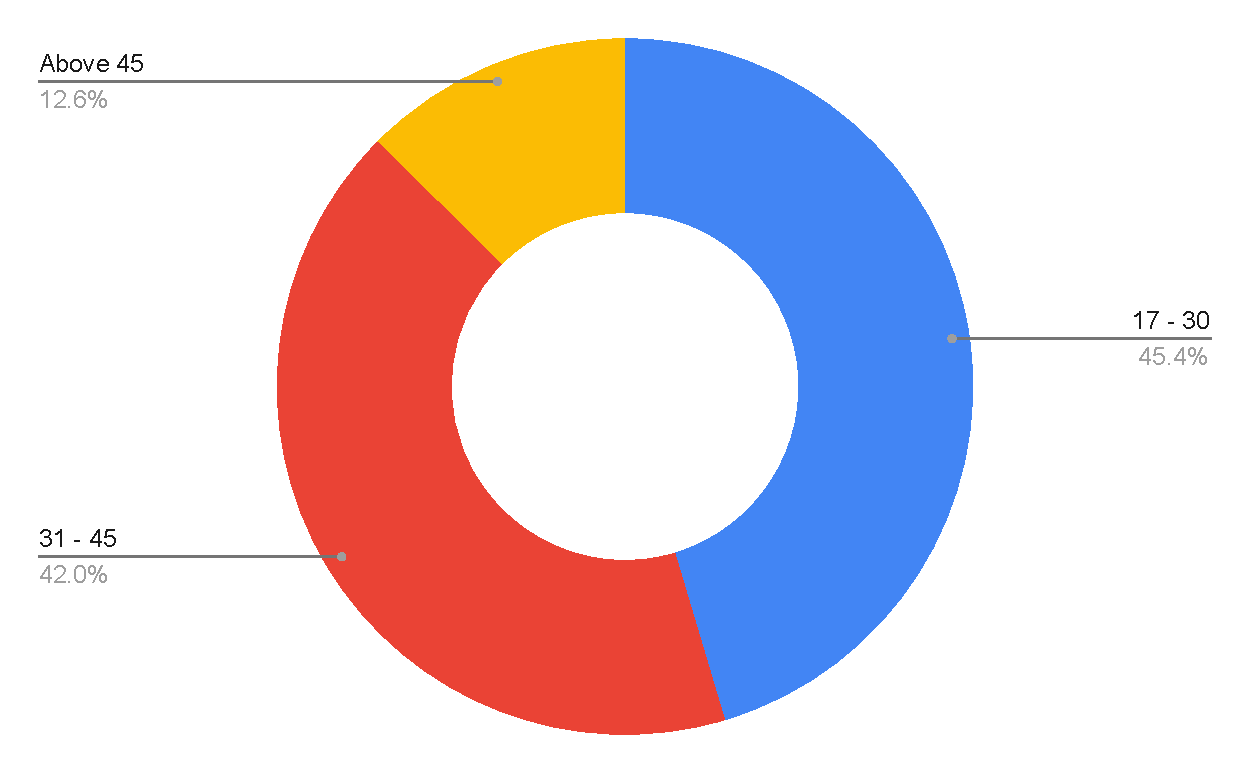
\includegraphics[width=13cm]{thesis/paper/images/p1_age.pdf}
  \textbf{Age distribution}
\end{figure}

\begin{figure}[H]
  \centering
  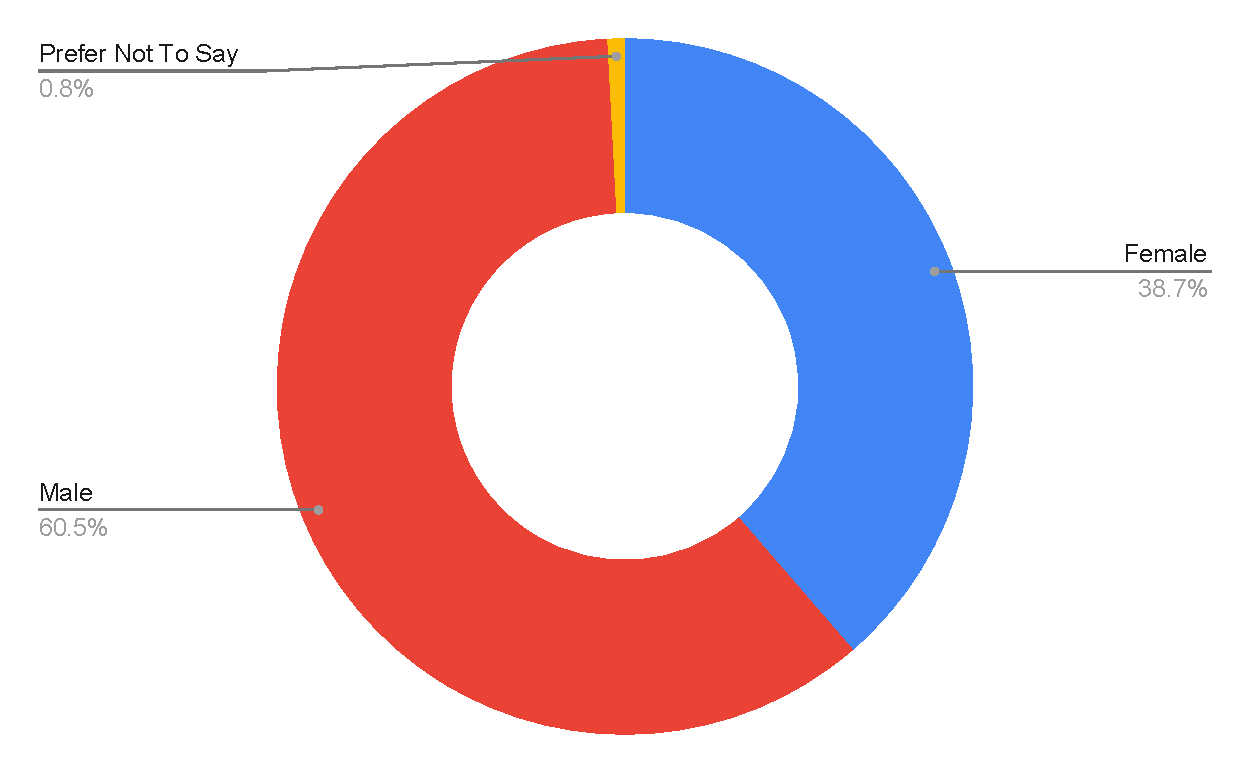
\includegraphics[width=13cm]{thesis/paper/images/p1_gender.pdf}
  \textbf{Gender distribution}
\end{figure}

\begin{figure}[H]
  \centering
  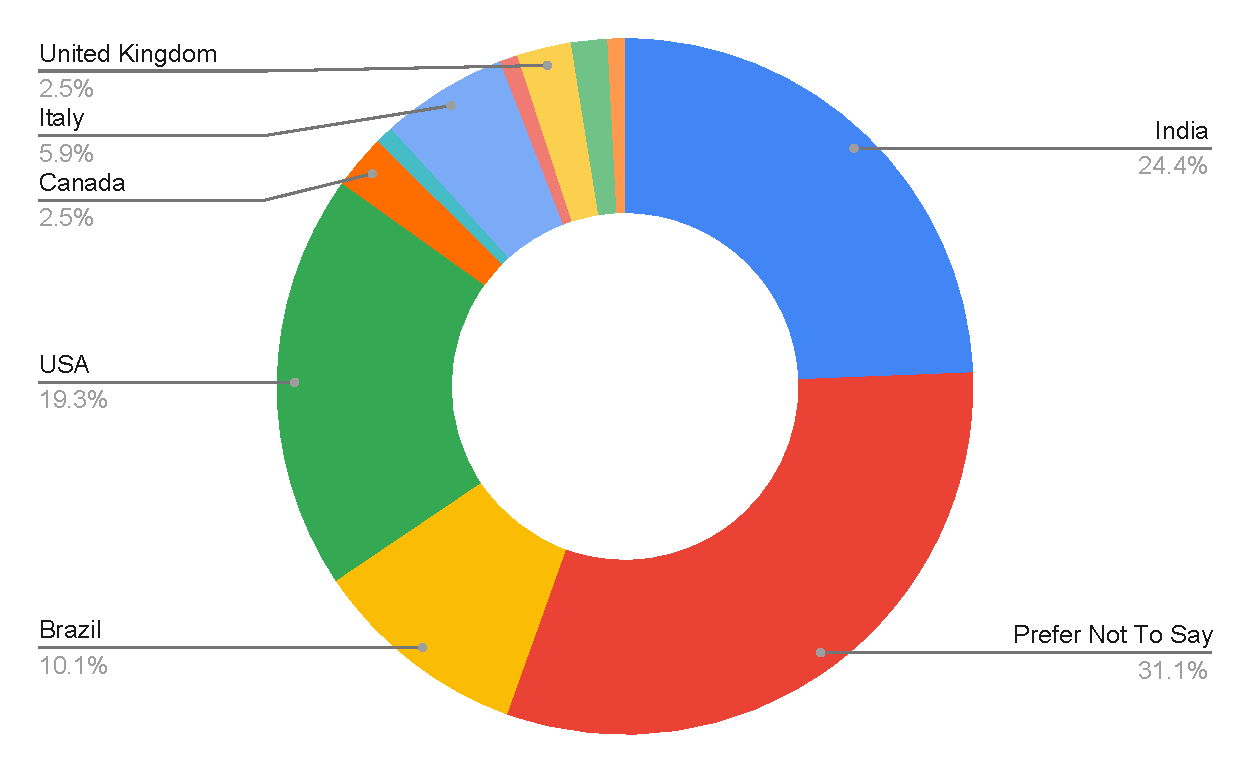
\includegraphics[width=13cm]{thesis/paper/images/p1_country.pdf}
  \textbf{Country of Origin}
\end{figure}

\begin{figure}[H]
  \centering
  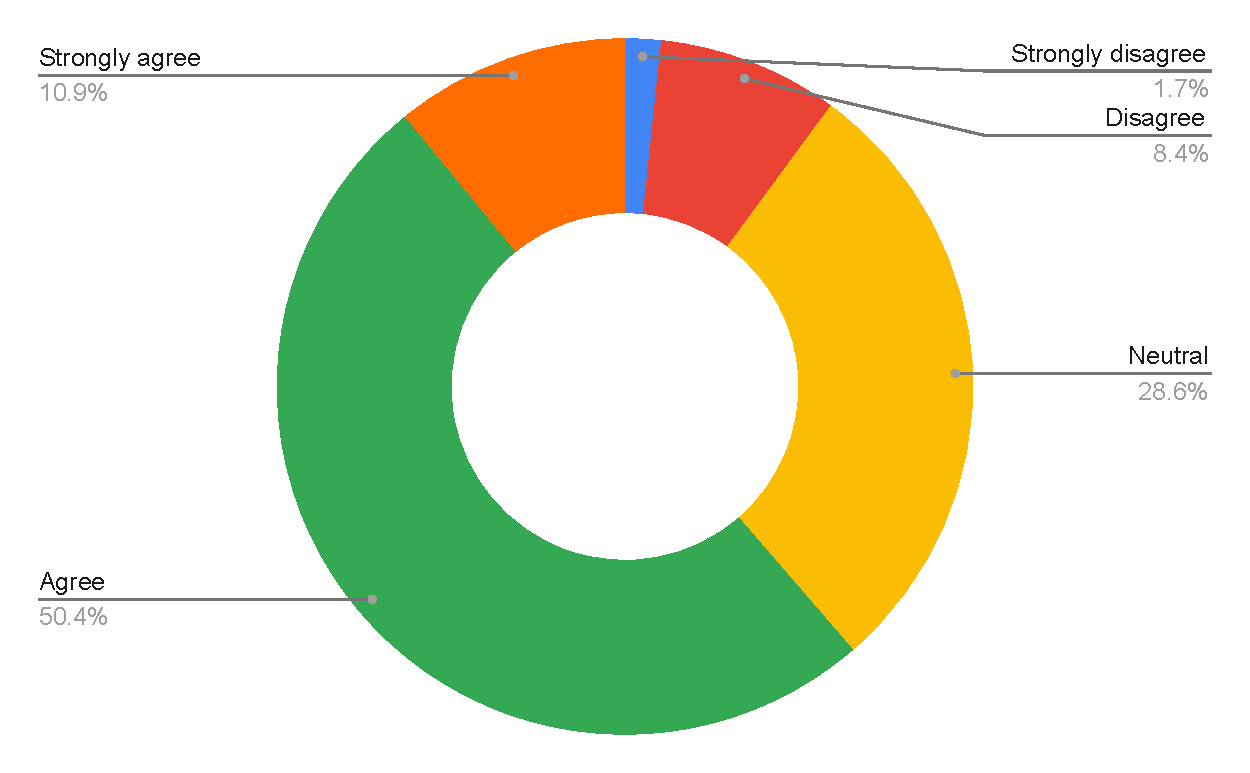
\includegraphics[width=13cm]{thesis/paper/images/p1_q1.pdf}
  \textbf{Question:} I experience UI/UX inconsistencies in some applications
\end{figure}

\begin{figure}[H]
  \centering
  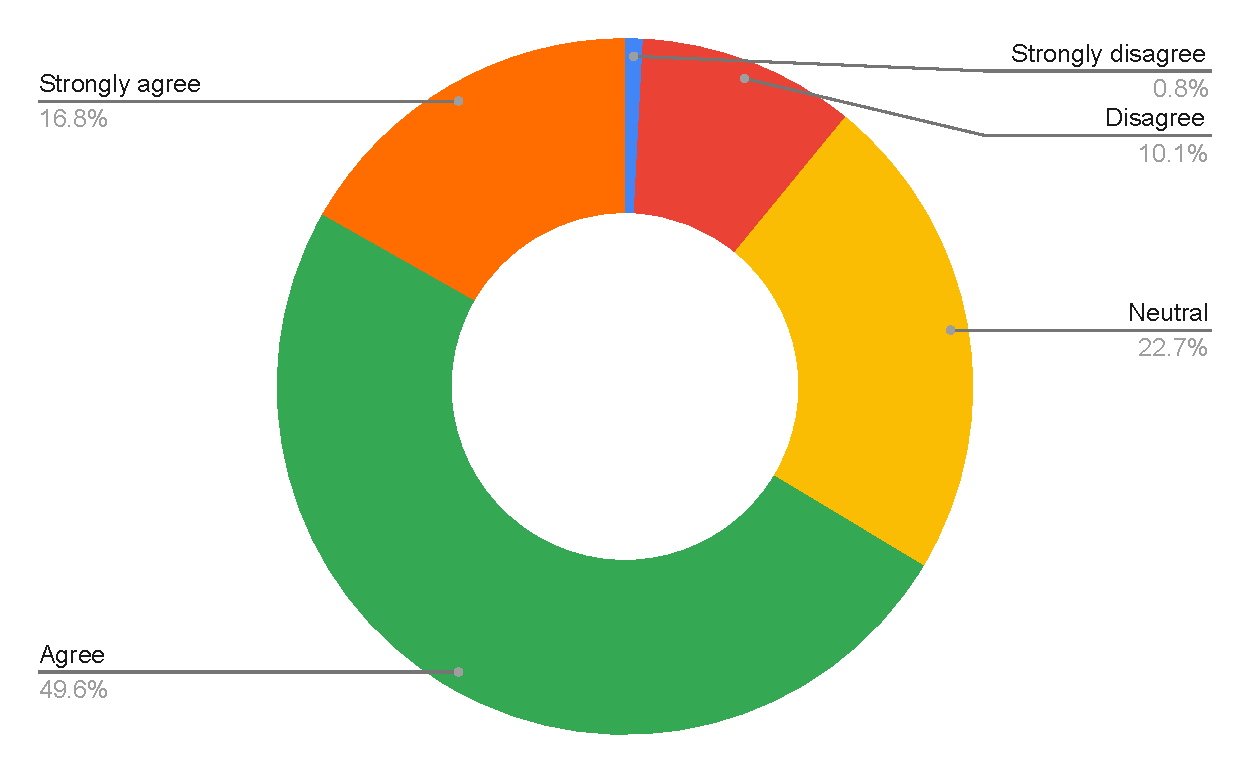
\includegraphics[width=13cm]{thesis/paper/images/p1_q2.pdf}
  \textbf{Question:} I sometimes experience poor design in some applications
\end{figure}

\begin{figure}[H]
  \centering
  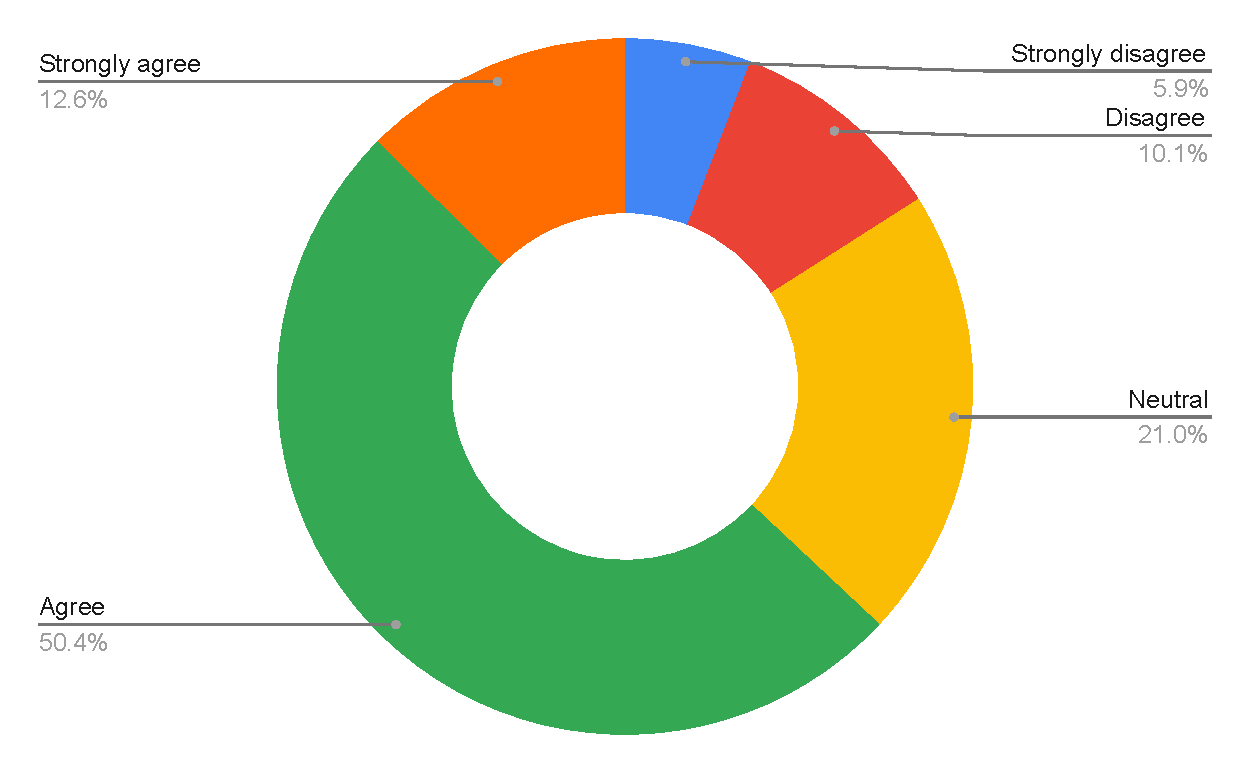
\includegraphics[width=13cm]{thesis/paper/images/p1_q3.pdf}
  \textbf{Question:} Advertisement sector is out of control
\end{figure}

\begin{figure}[H]
  \centering
  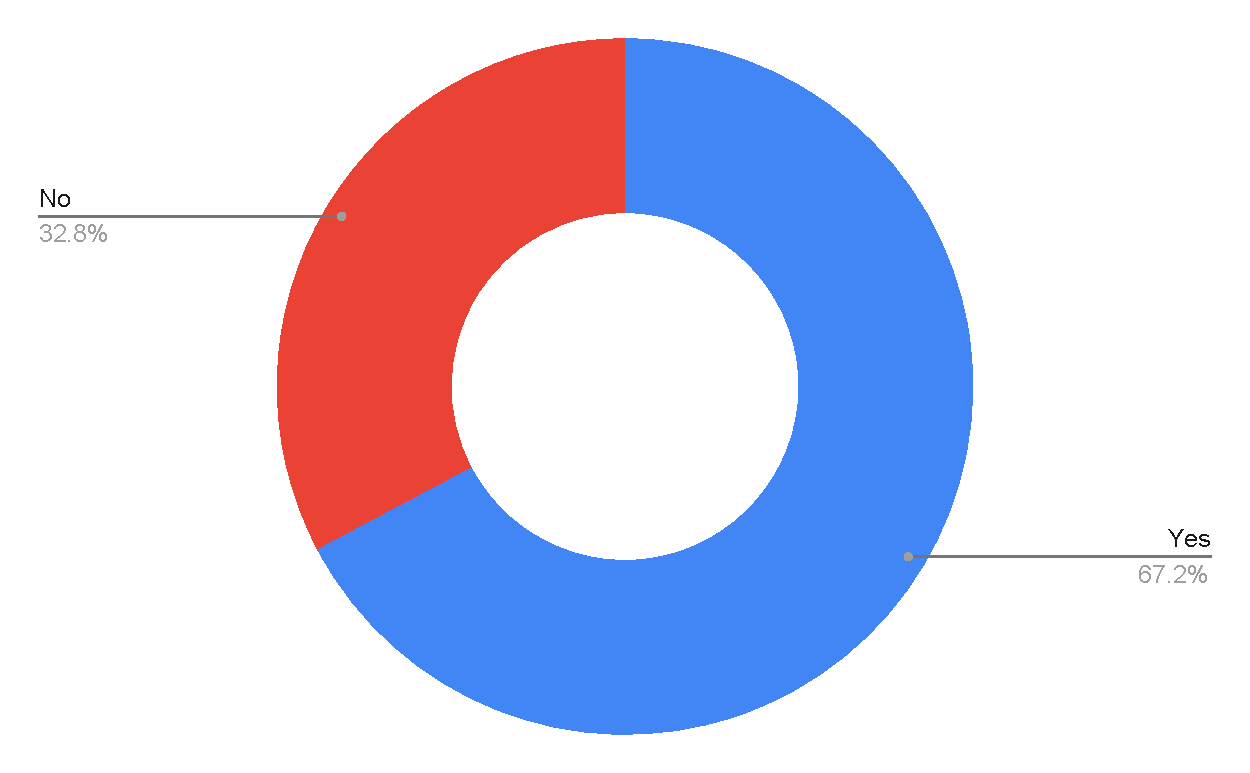
\includegraphics[width=13cm]{thesis/paper/images/p1_q4.pdf}
  \textbf{Question:} I use an AdBlocker
\end{figure}

\begin{figure}[H]
  \centering
  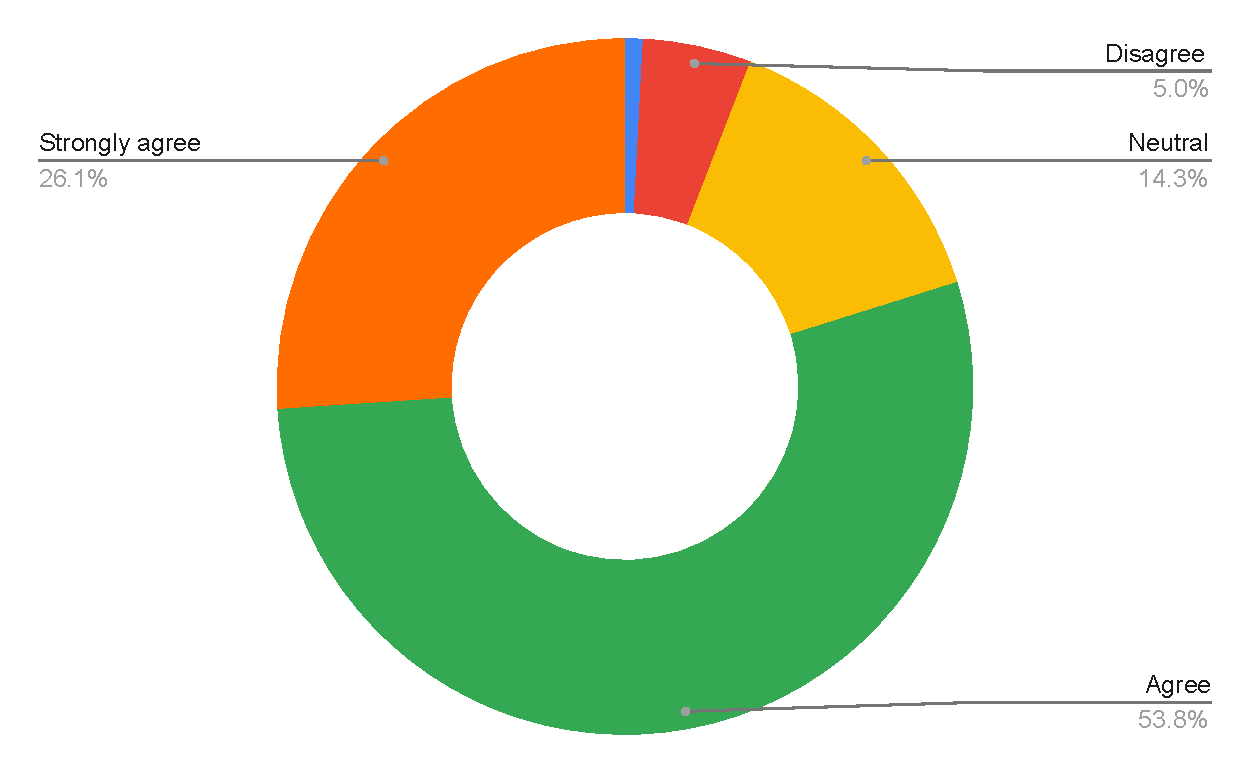
\includegraphics[width=13cm]{thesis/paper/images/p1_q5.pdf}
  \textbf{Question:} I'm often frustrated with ads on the internet
\end{figure}

\begin{figure}[H]
  \centering
  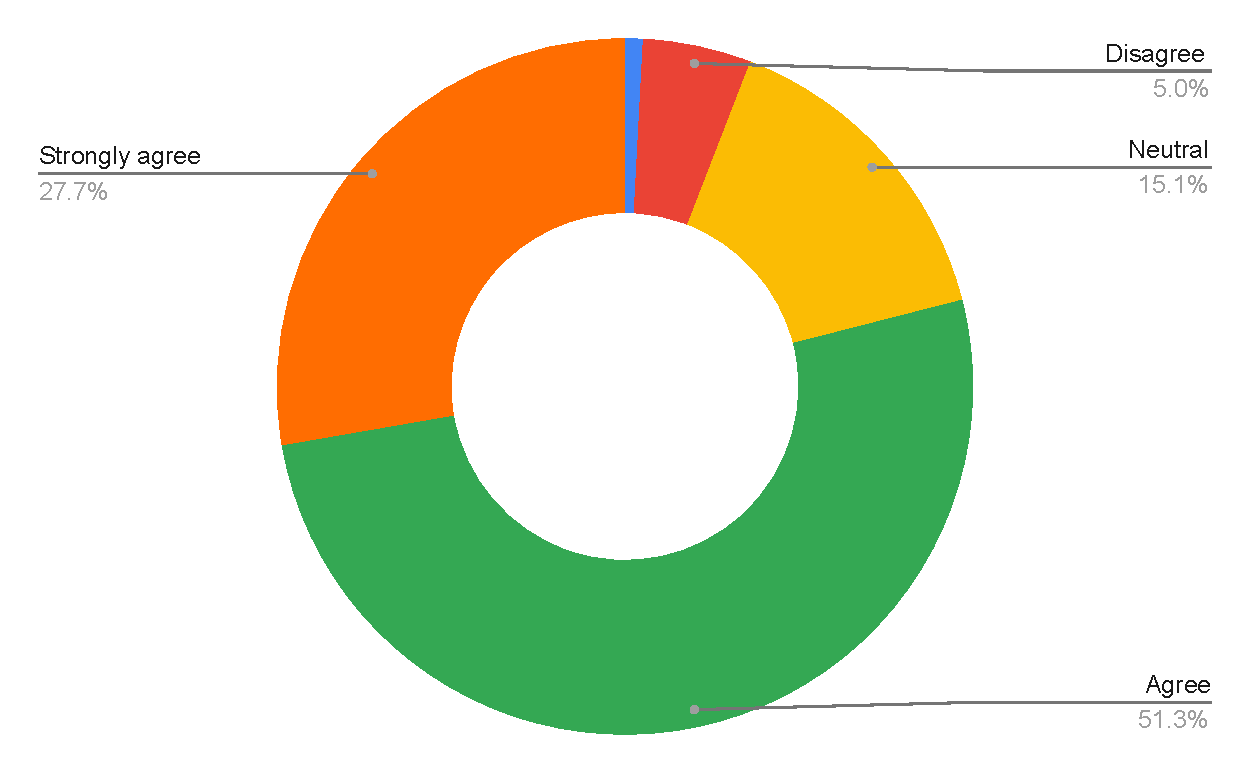
\includegraphics[width=13cm]{thesis/paper/images/p1_q6.pdf}
  \textbf{Question:} I'm often frustrated with ads on mobile/desktop apps
\end{figure}

\begin{figure}[H]
  \centering
  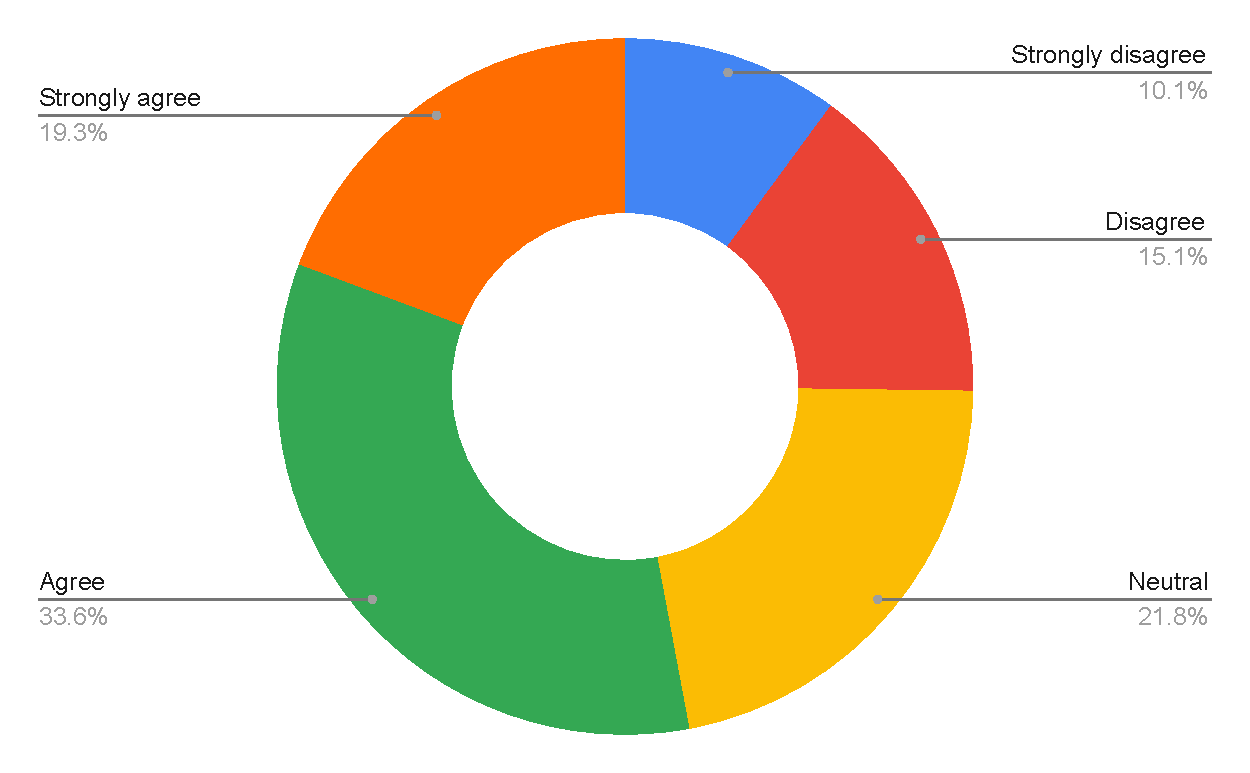
\includegraphics[width=13cm]{thesis/paper/images/p1_q7.pdf}
  \textbf{Question:} I would rather pay a small fee than seeing ads
\end{figure}

\begin{figure}[H]
  \centering
  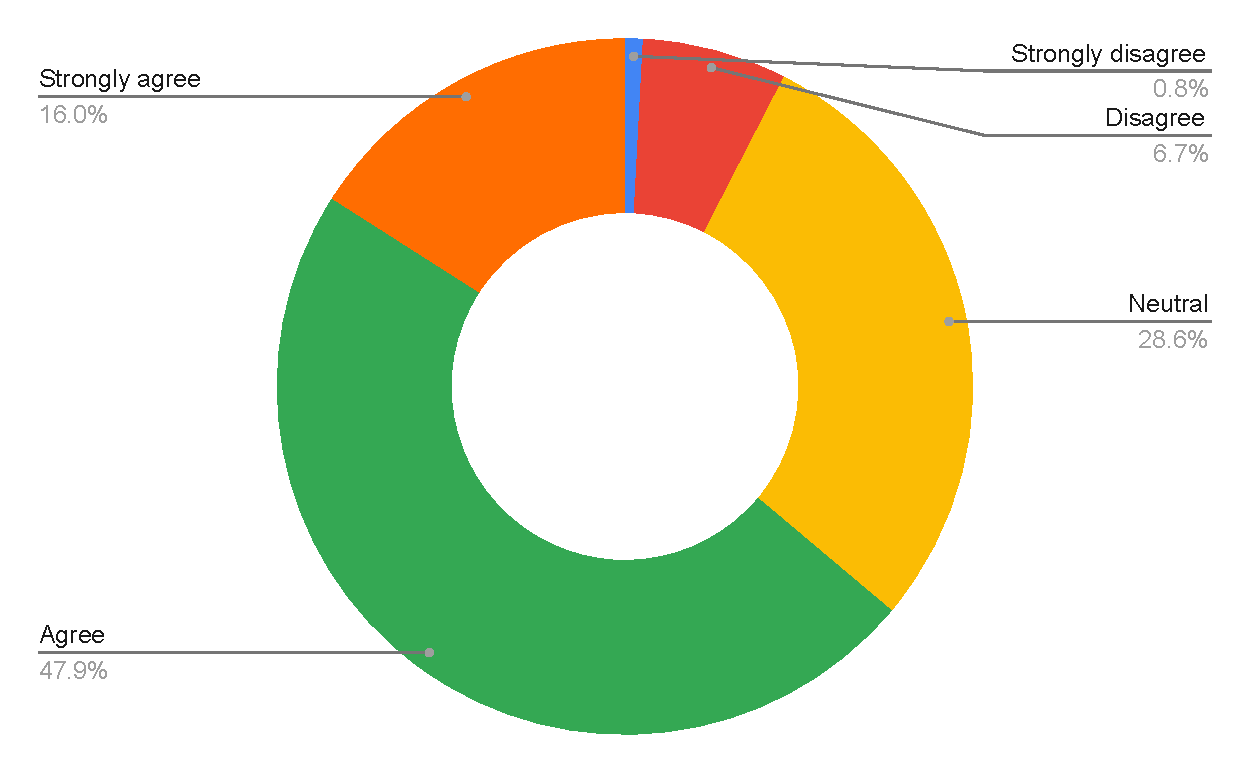
\includegraphics[width=13cm]{thesis/paper/images/p1_q8.pdf}
  \textbf{Question:} I wish I was able to customise the appearances of websites/applications.
\end{figure}

\begin{figure}[H]
  \centering
  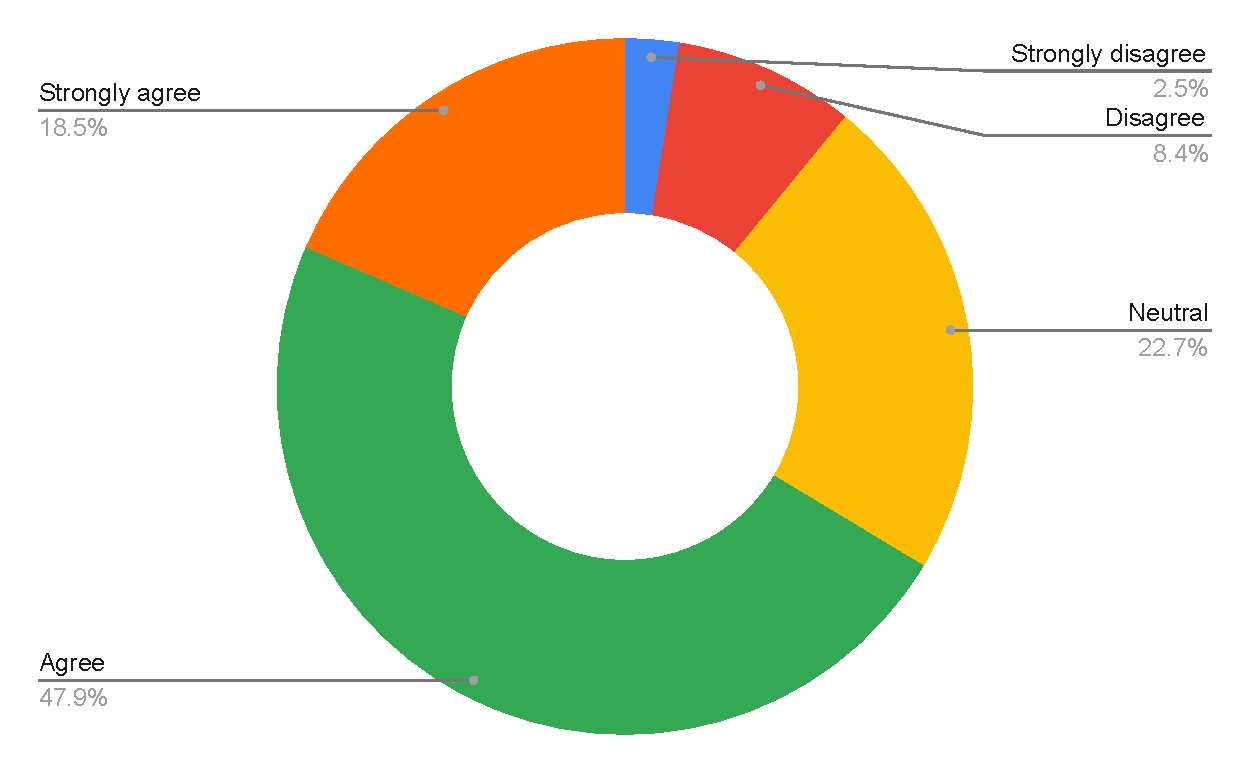
\includegraphics[width=13cm]{thesis/paper/images/p1_q9.pdf}
  \textbf{Question:} I wish I could choose or create a universal theme that would apply to all websites/applications
\end{figure}

\begin{figure}[H]
  \centering
  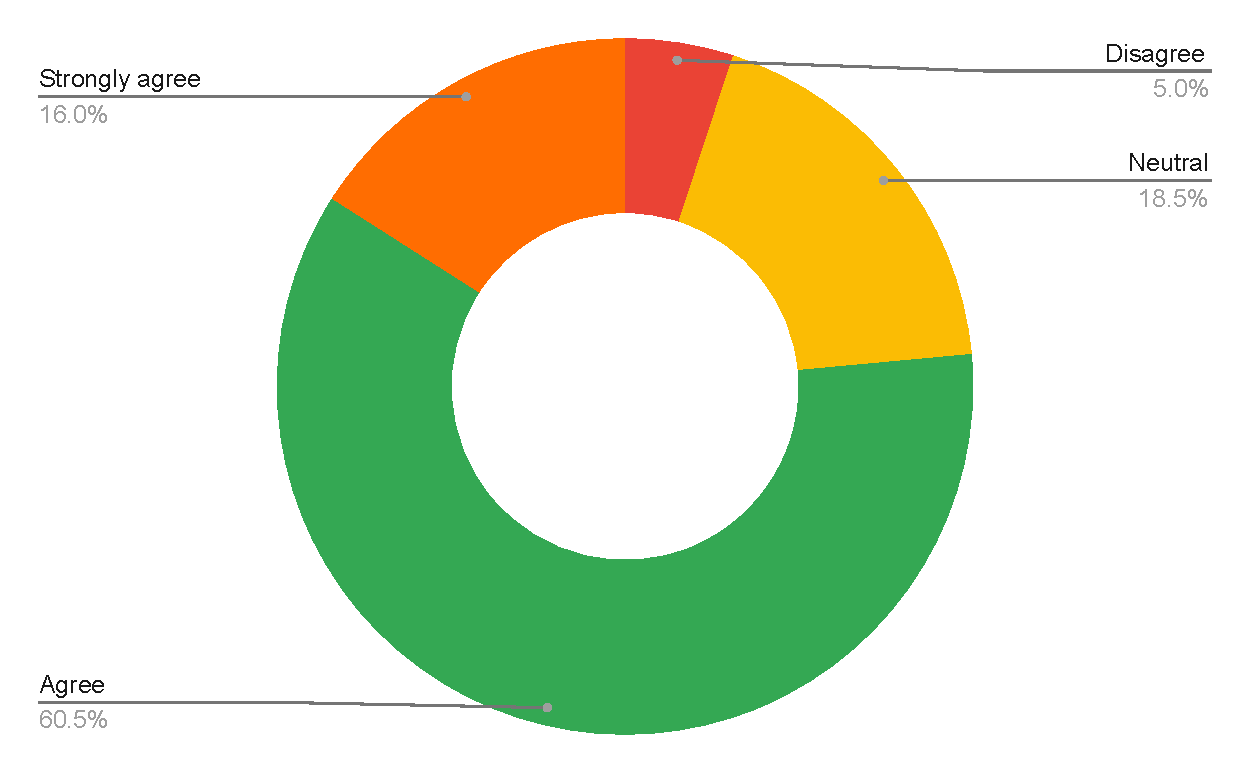
\includegraphics[width=13cm]{thesis/paper/images/p1_q10.pdf}
  \textbf{Question:} Applications I use on a daily basis are mostly available on all my devices/platforms
\end{figure}

\begin{figure}[H]
  \centering
  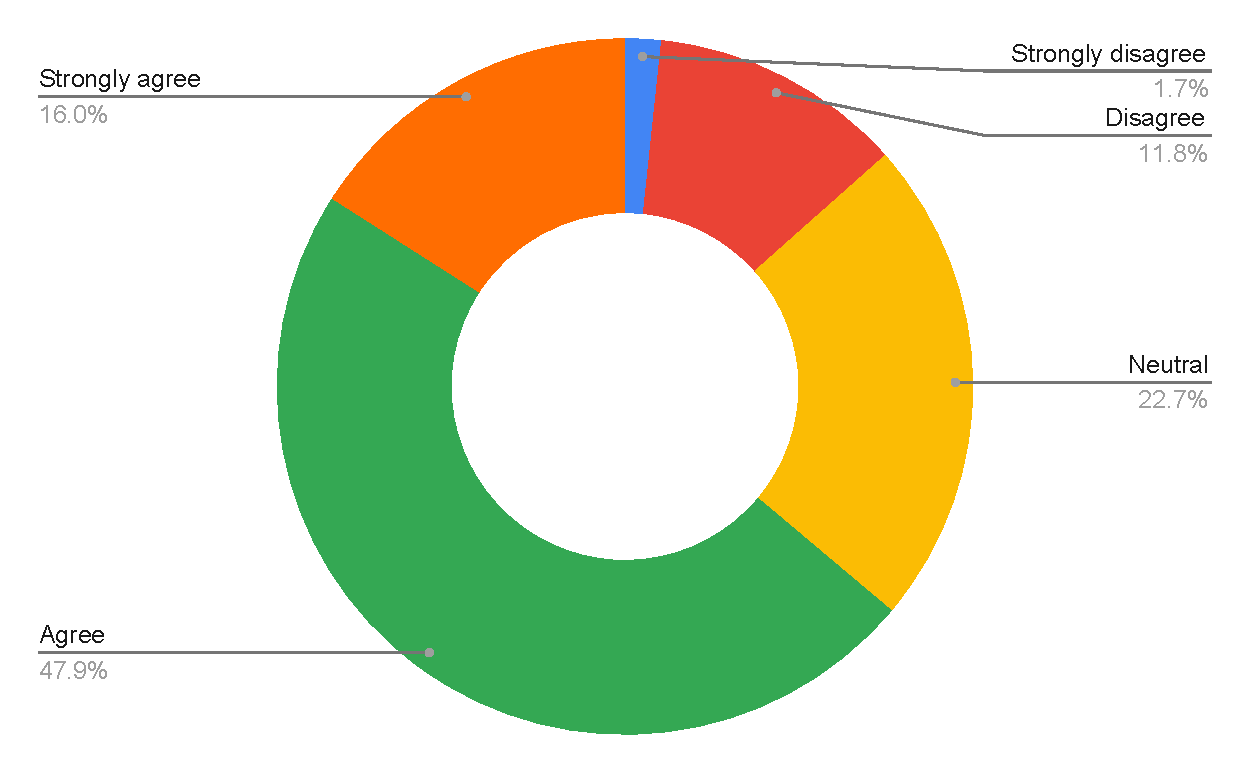
\includegraphics[width=13cm]{thesis/paper/images/p1_q11.pdf}
  \textbf{Question:} Occasionally I have to use desktop applications that are not optimised for small screens/touch interfaces on my phone
\end{figure}

\begin{figure}[H]
  \centering
  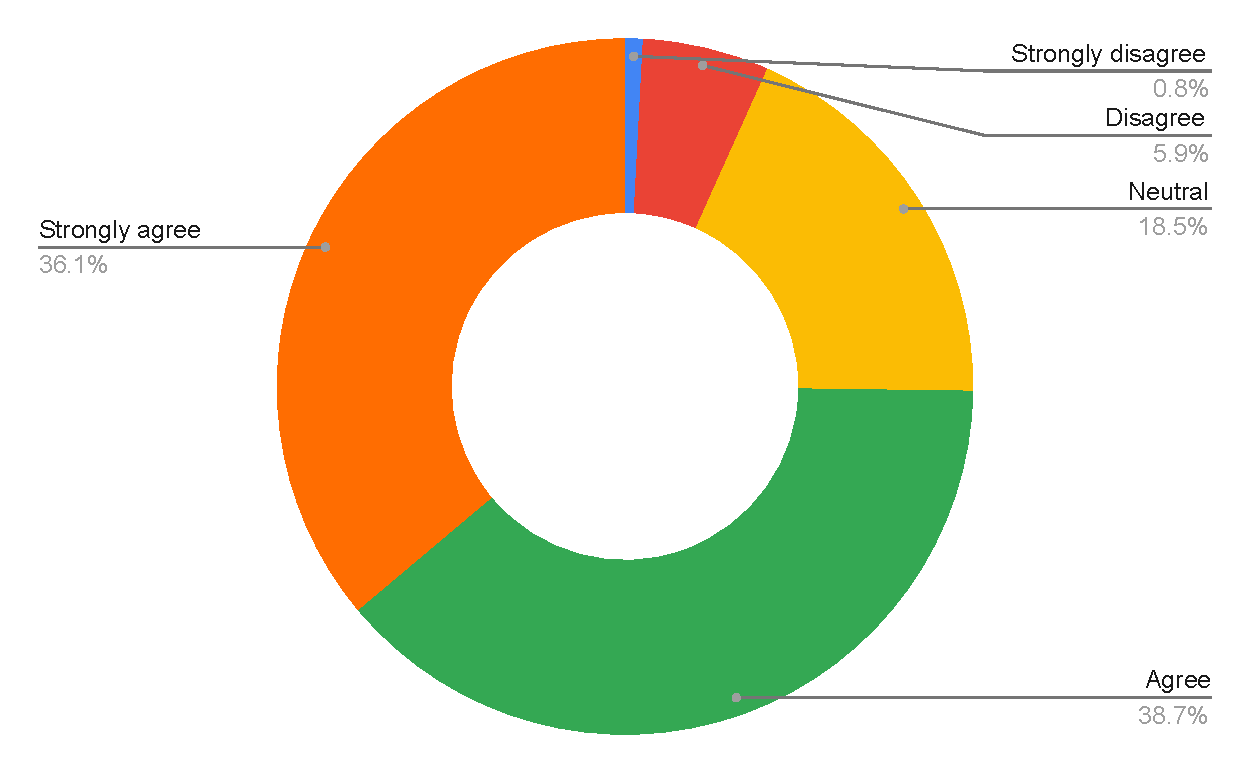
\includegraphics[width=13cm]{thesis/paper/images/p1_q12.pdf}
  \textbf{Question:} If I'm going to use a service just for once, I prefer using their website instead of downloading their application on my phone
\end{figure}

\begin{figure}[H]
  \centering
  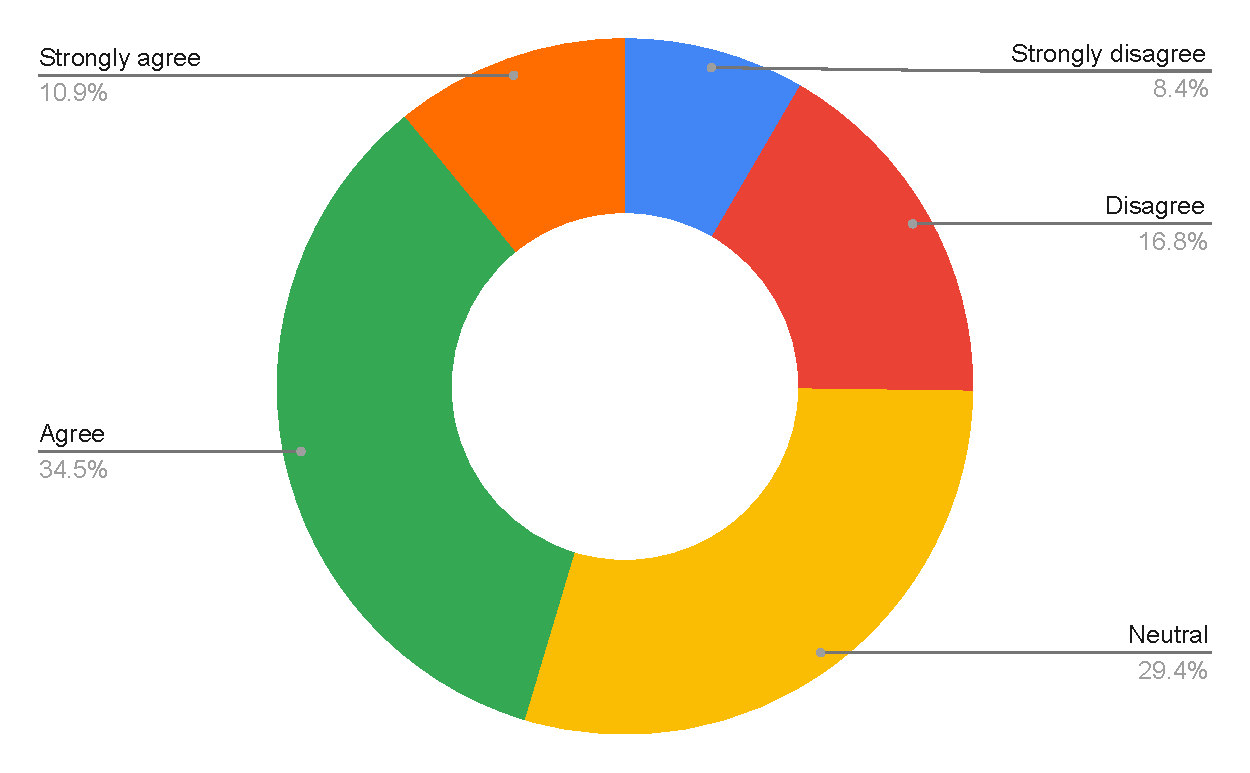
\includegraphics[width=13cm]{thesis/paper/images/p1_q13.pdf}
  \textbf{Question:} I feel safe on the internet
\end{figure}

\begin{figure}[H]
  \centering
  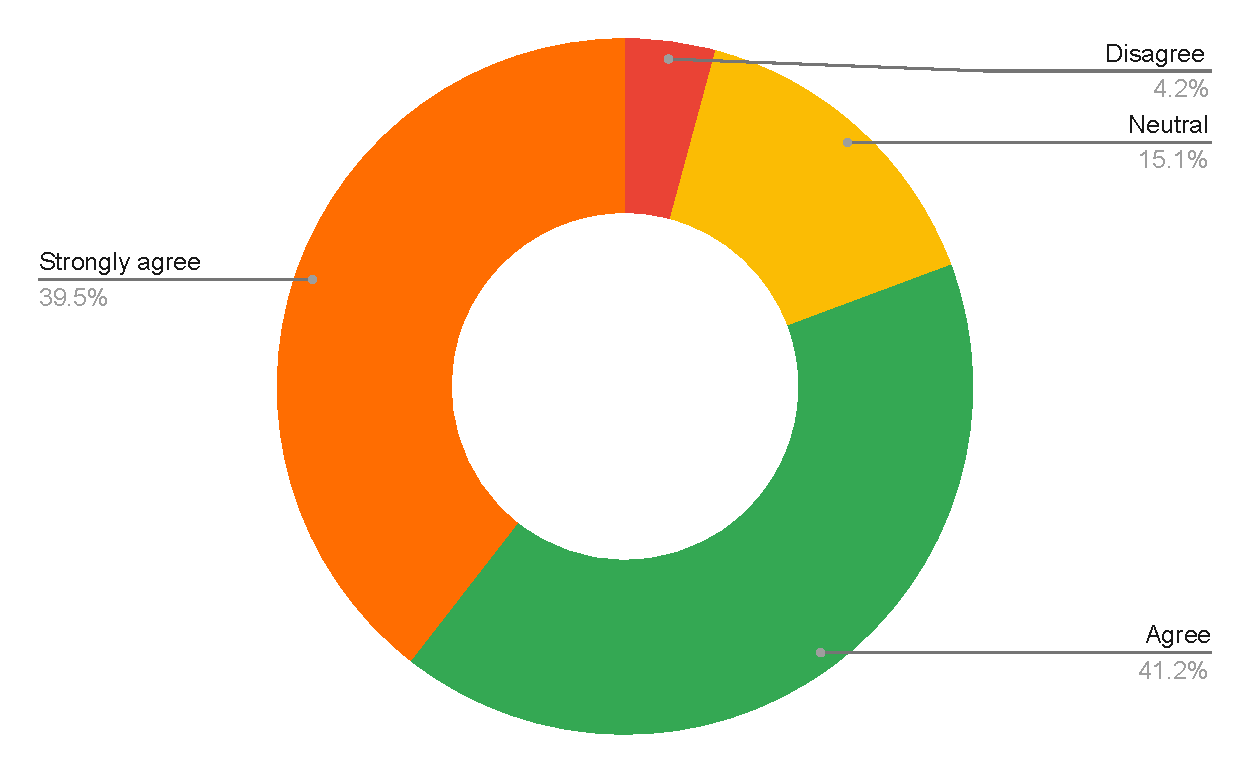
\includegraphics[width=13cm]{thesis/paper/images/p1_q14.pdf}
  \textbf{Question:} I care about my privacy on the internet
\end{figure}

\begin{figure}[H]
  \centering
  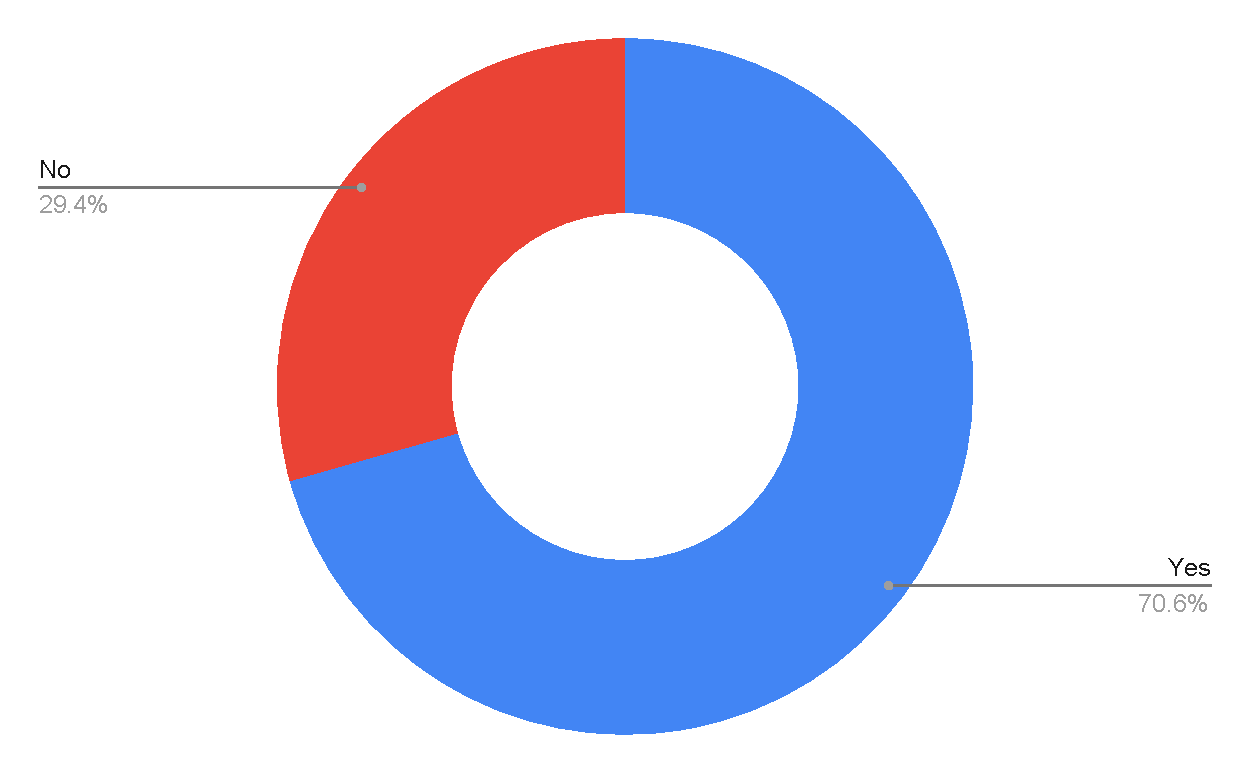
\includegraphics[width=13cm]{thesis/paper/images/p1_q15.pdf}
  \textbf{Question:} Me, or someone I know was targeted by malicious software before
\end{figure}

\begin{figure}[H]
  \centering
  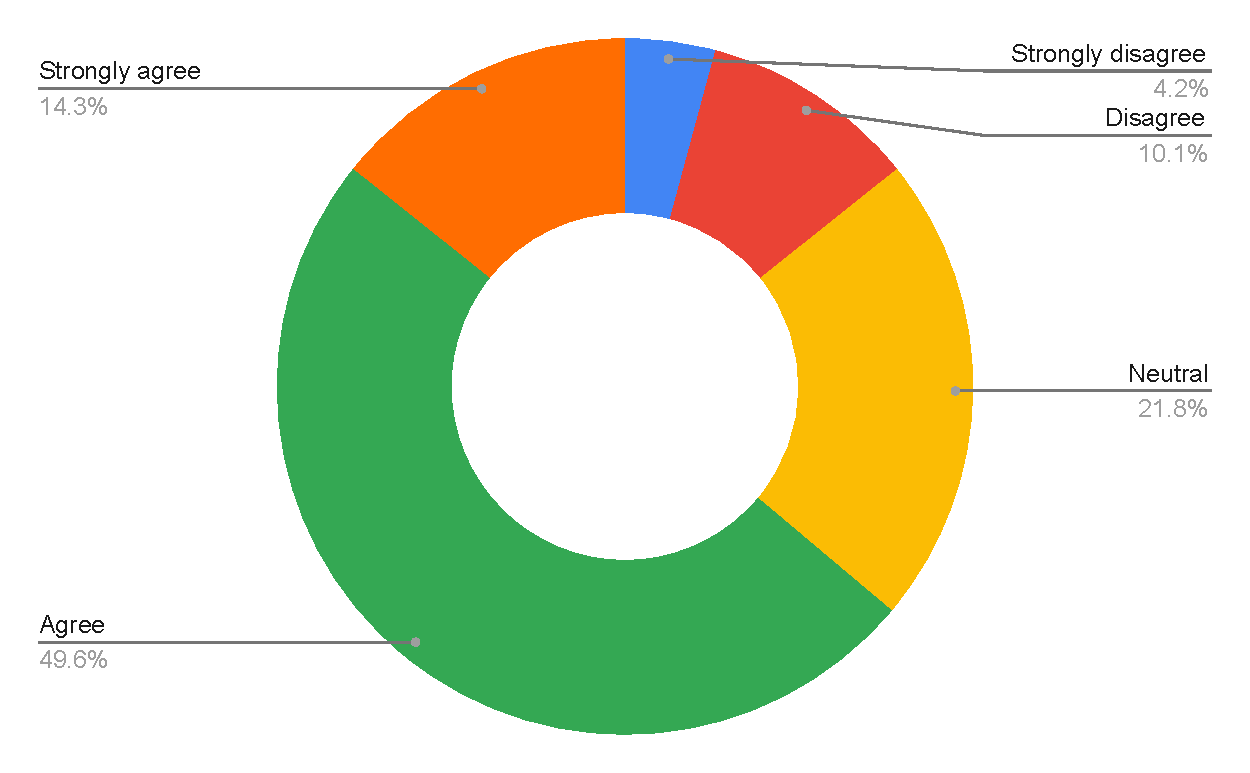
\includegraphics[width=13cm]{thesis/paper/images/p1_q16.pdf}
  \textbf{Question:} I would rather pay a small fee than paying with my data
\end{figure}


\newpage
\subsection{Phase 2 Results}

As mentioned in the previous section, we conducted two separate questionnaire targeting end-users and developers for phase two of our user survey. After removing duplicate submissions and responses with invalid worker ids, we were left with 54 submissions for the end-uses survey, and 14 for the developer survey. Below, we present the response data for answers to each question, with the question text underneath with an indication for which survey the question is from. For both surveys, we include age, country and gender data. For the developer survey, we additionally include years of experience as well.


\begin{figure}[H]
  \centering
  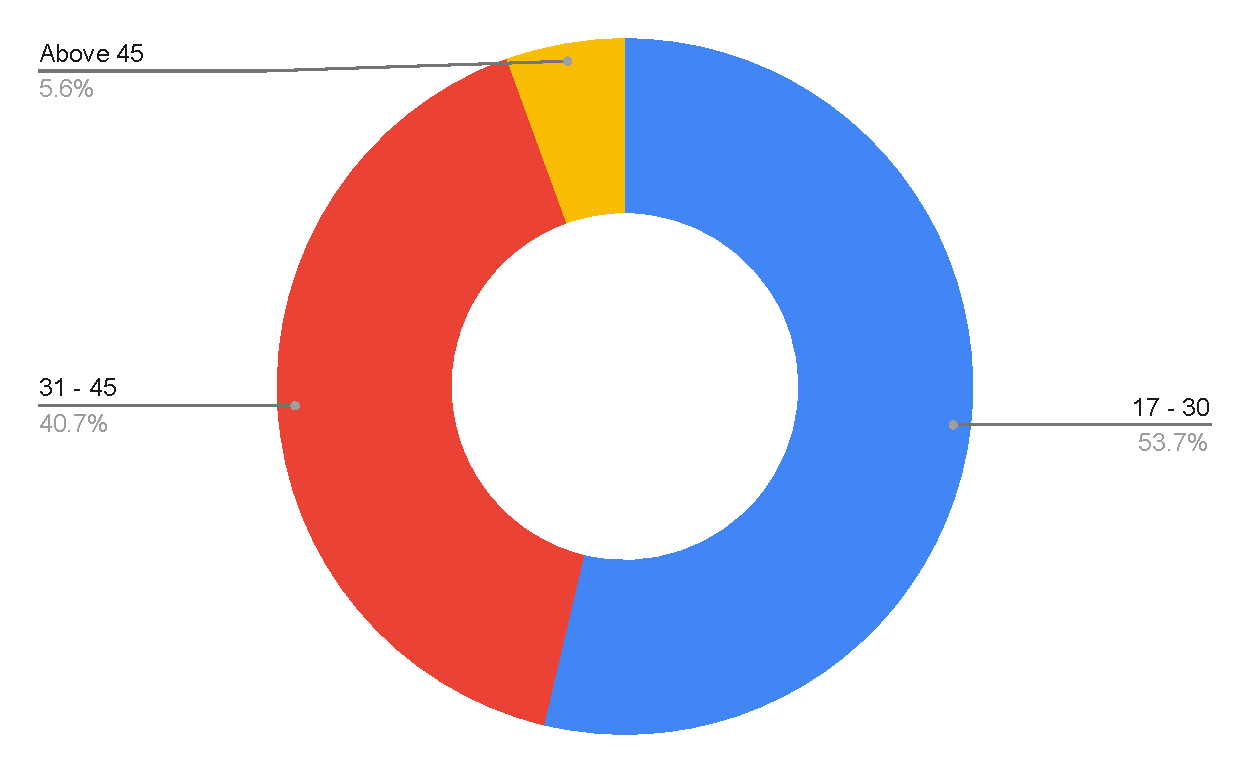
\includegraphics[width=13cm]{thesis/paper/images/p2u_age.pdf}
  \textbf{Age distribution (End-user survey)}
\end{figure}


\begin{figure}[H]
  \centering
  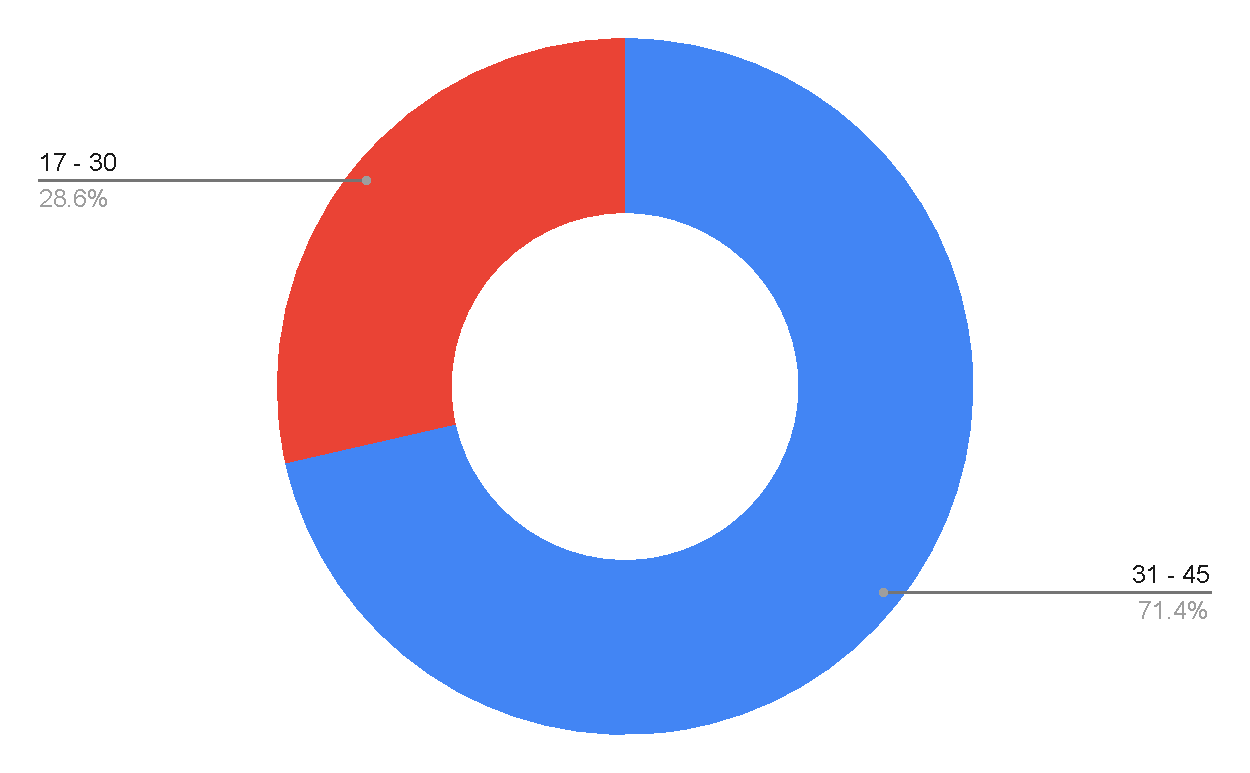
\includegraphics[width=13cm]{thesis/paper/images/p2d_age.pdf}
  \textbf{Age distribution (Developer survey)}
\end{figure}

\begin{figure}[H]
  \centering
  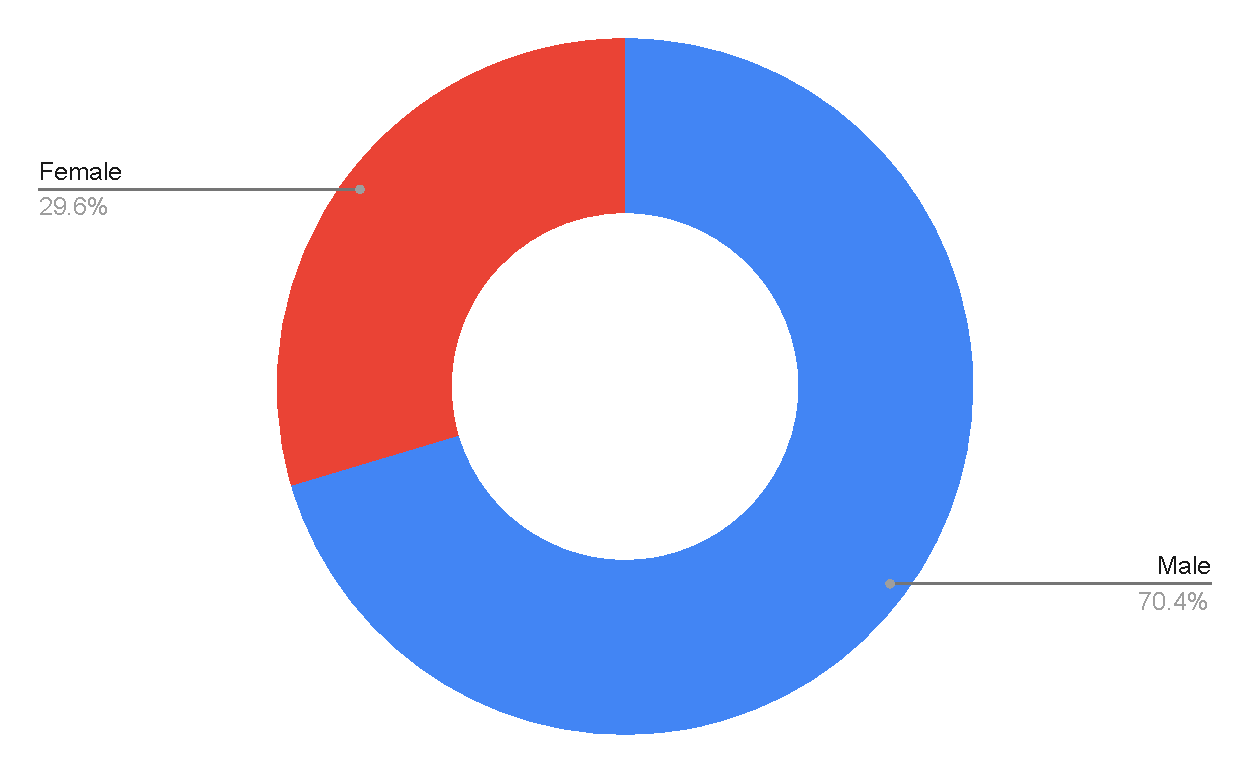
\includegraphics[width=13cm]{thesis/paper/images/p2u_gender.pdf}
  \textbf{Gender distribution (End-user survey)}
\end{figure}

\begin{figure}[H]
  \centering
  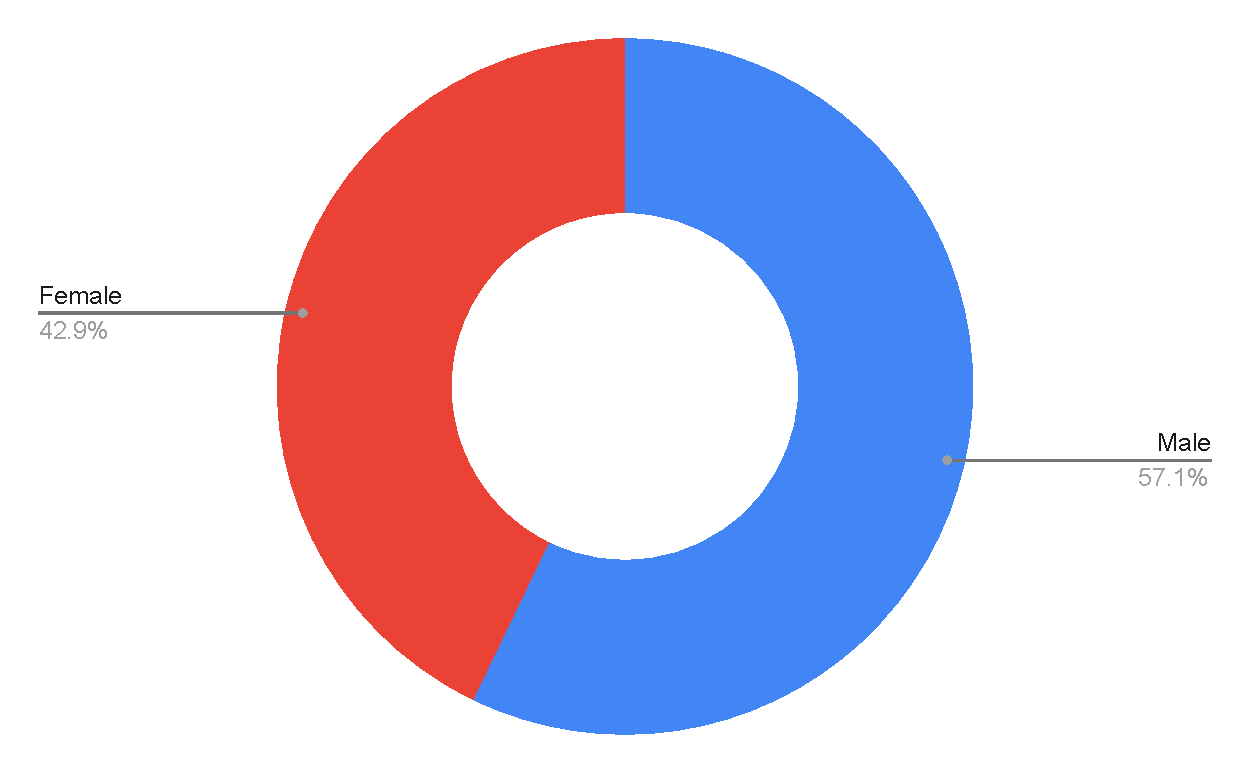
\includegraphics[width=13cm]{thesis/paper/images/p2d_gender.pdf}
  \textbf{Gender distribution (Developer survey)}
\end{figure}

\begin{figure}[H]
  \centering
  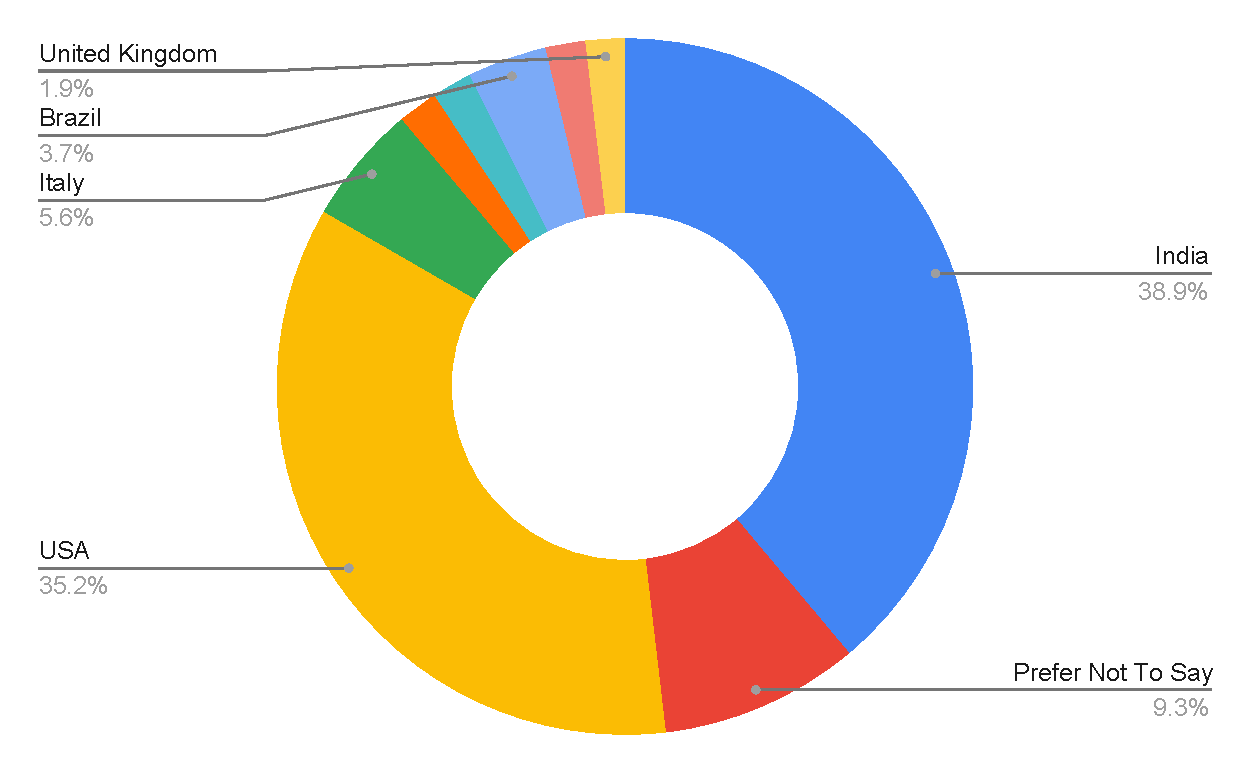
\includegraphics[width=13cm]{thesis/paper/images/p2u_country.pdf}
  \textbf{Country of Origin (End-user survey)}
\end{figure}

\begin{figure}[H]
  \centering
  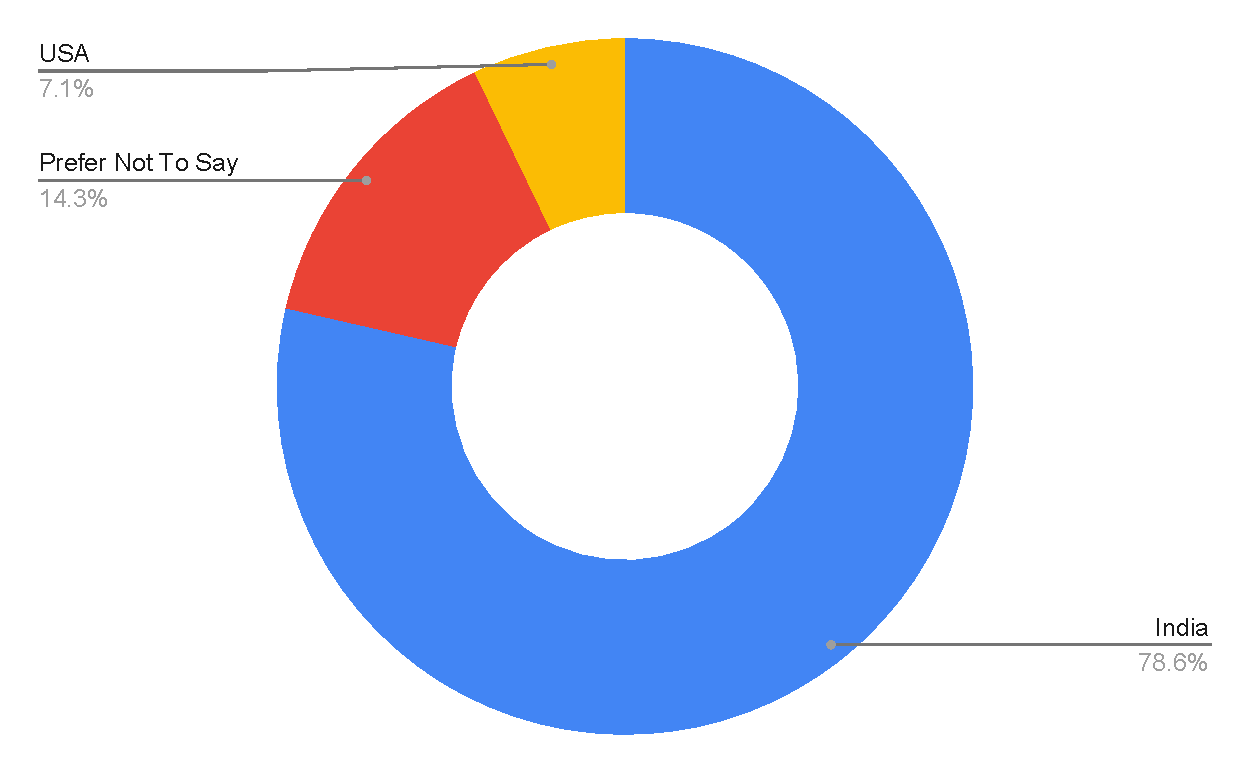
\includegraphics[width=13cm]{thesis/paper/images/p2d_country.pdf}
  \textbf{Country of Origin (Developer survey)}
\end{figure}

\begin{figure}[H]
  \centering
  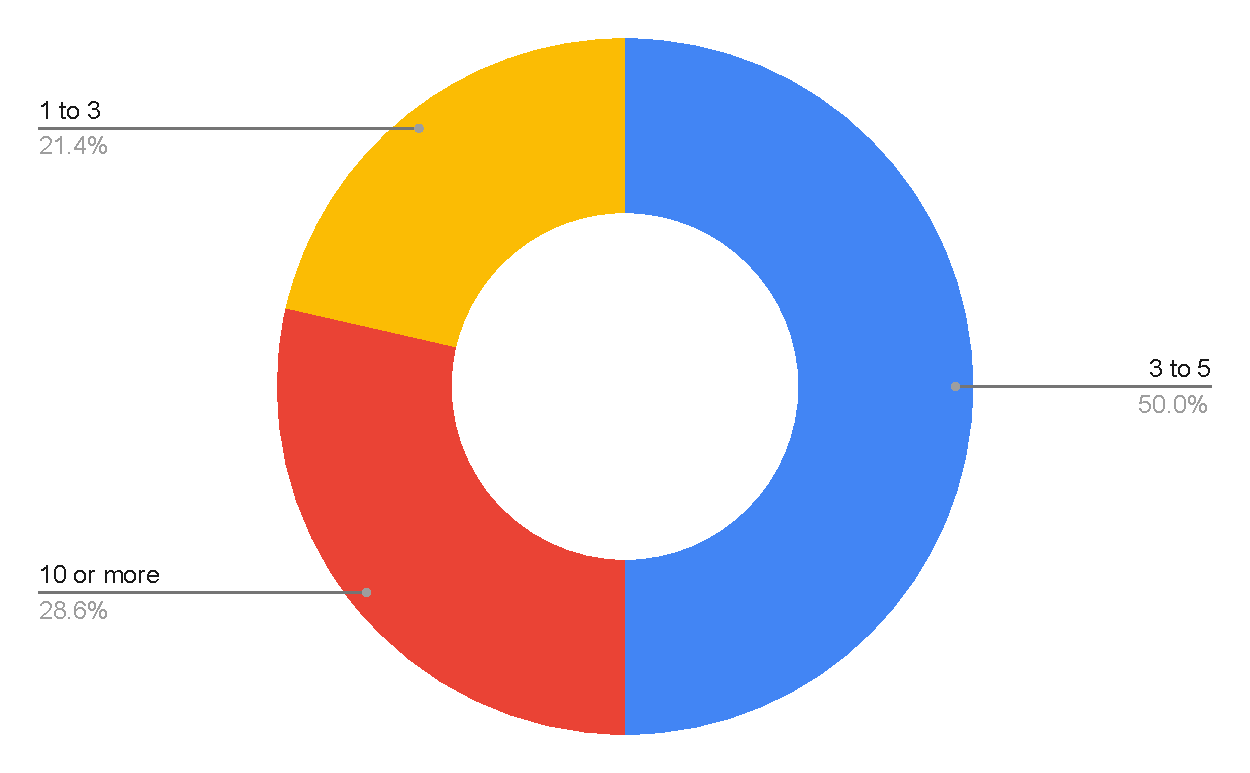
\includegraphics[width=13cm]{thesis/paper/images/p2d_experience.pdf}
  \textbf{Years of Experience (Developer survey)}
\end{figure}

\begin{figure}[H]
  \centering
  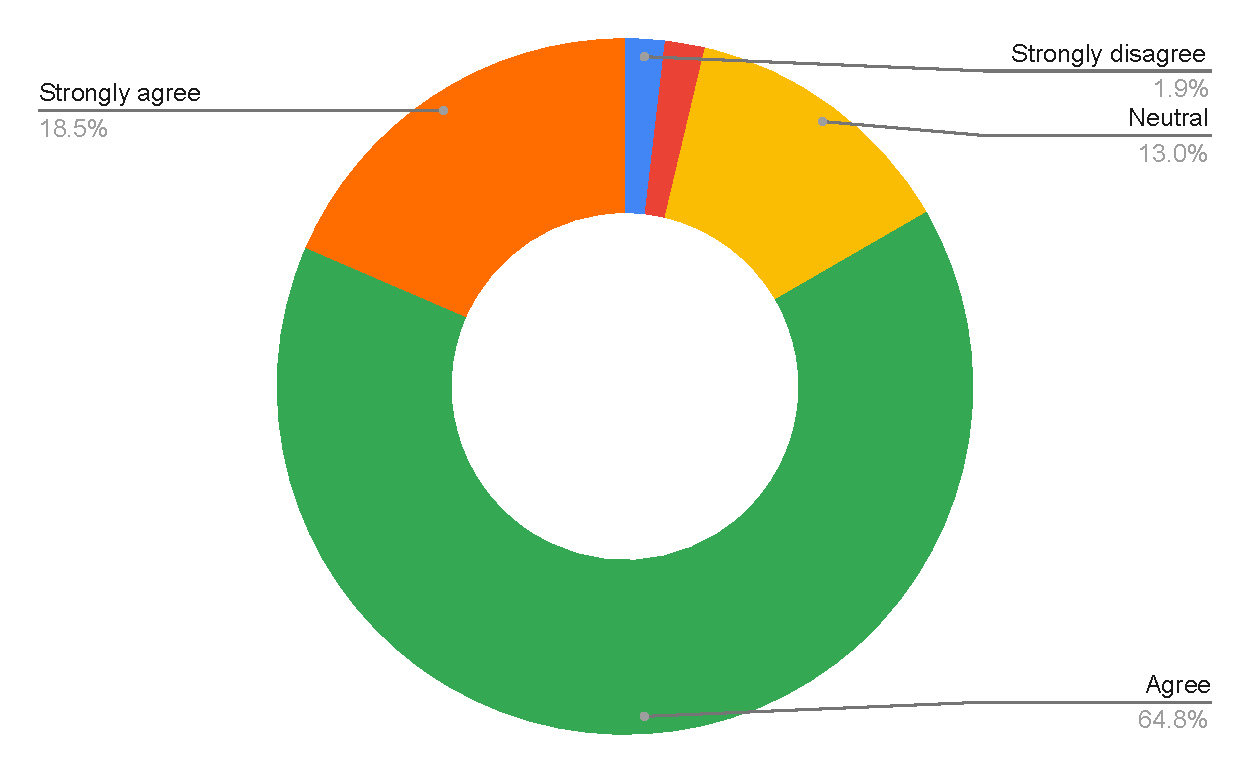
\includegraphics[width=13cm]{thesis/paper/images/p2u_q1.pdf}
  \textbf{Question (End-user survey):} Standardised UI components will improve the consistency across front-end applications
\end{figure}

\begin{figure}[H]
  \centering
  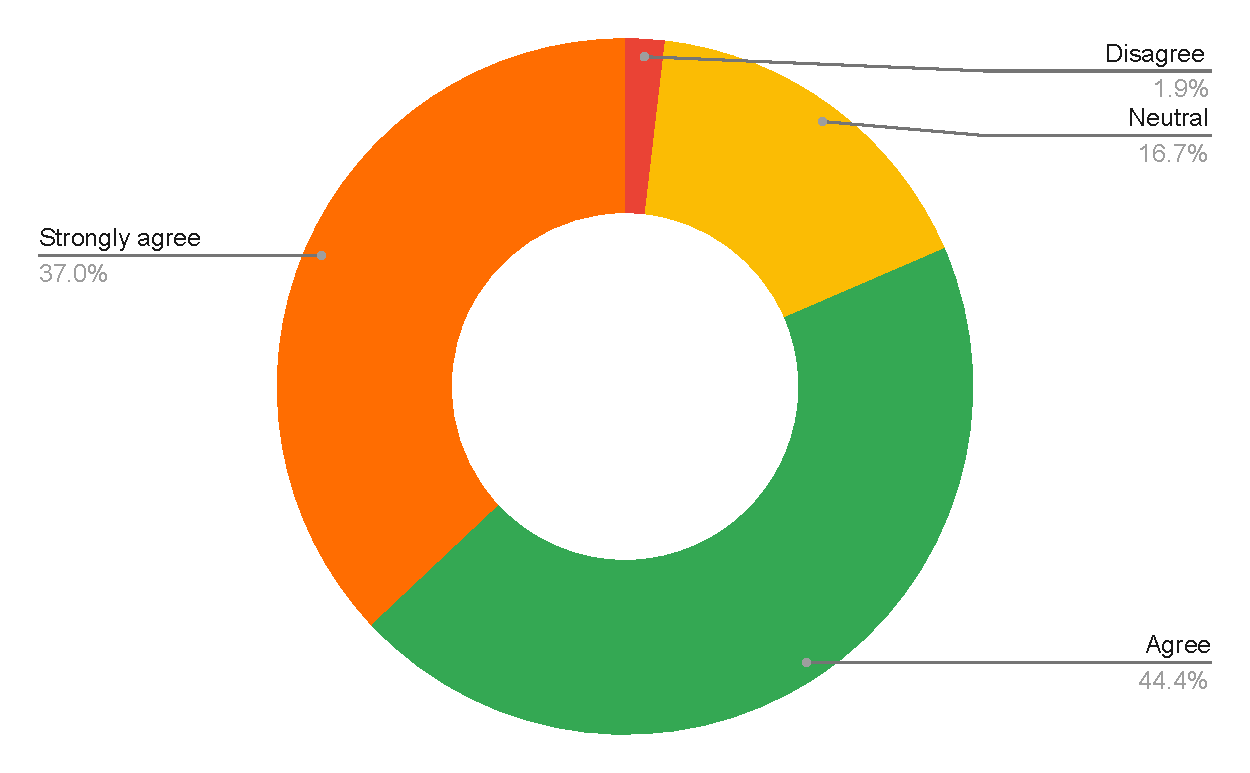
\includegraphics[width=13cm]{thesis/paper/images/p2u_q2.pdf}
  \textbf{Question (End-user survey):} I prefer consistency over variability
\end{figure}

\begin{figure}[H]
  \centering
  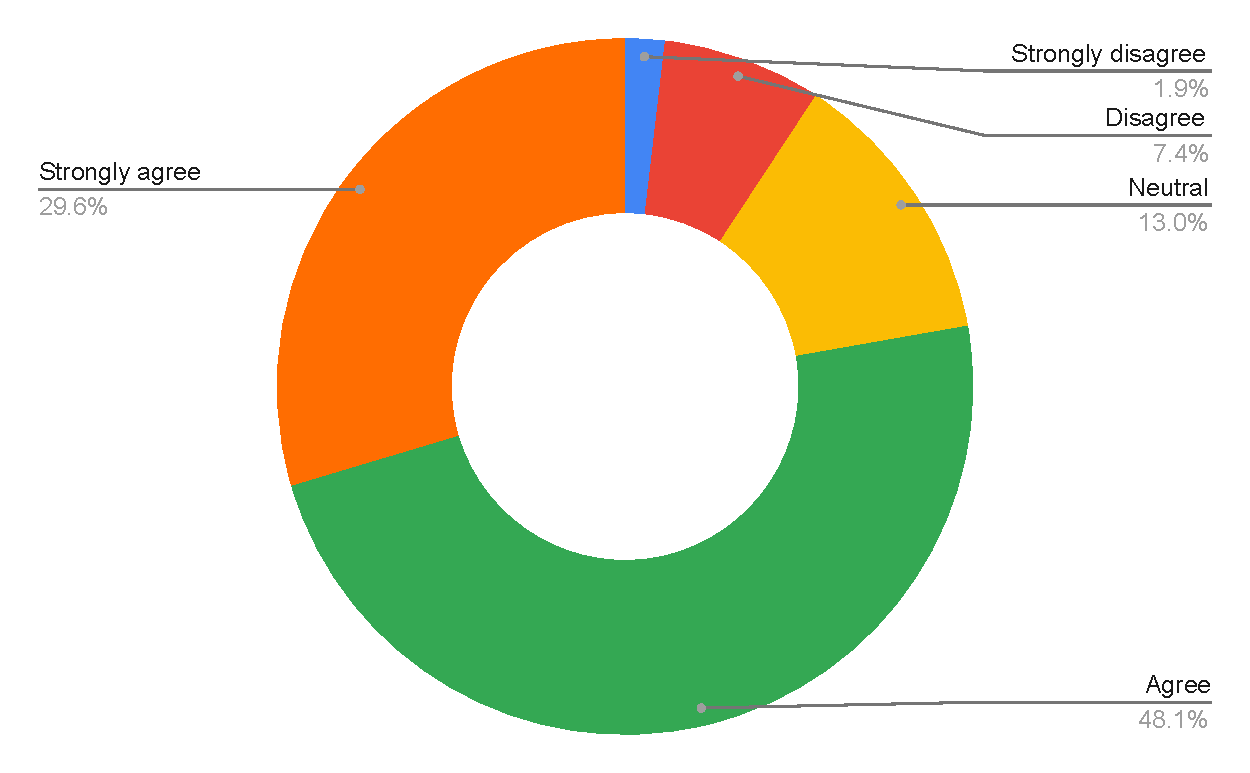
\includegraphics[width=13cm]{thesis/paper/images/p2u_q3.pdf}
  \textbf{Question (End-user survey):} I prefer advertisements to blend in naturally to the look-and-feel of the website instead of sticking out
\end{figure}

\begin{figure}[H]
  \centering
  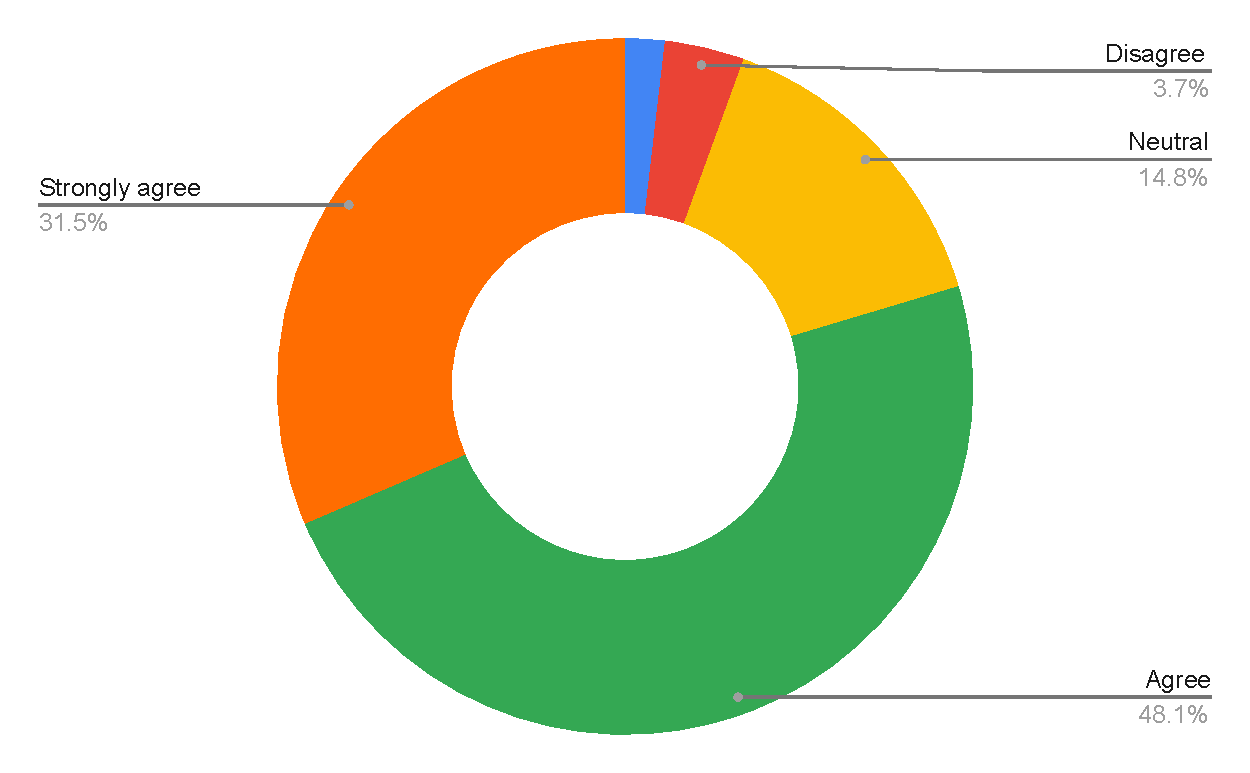
\includegraphics[width=13cm]{thesis/paper/images/p2u_q4.pdf}
  \textbf{Question (End-user survey):} I am okay with seeing non-intrusive and respectful advertisement (with no compromise of privacy), OR paying a small fee in order to support the creator
\end{figure}

\begin{figure}[H]
  \centering
  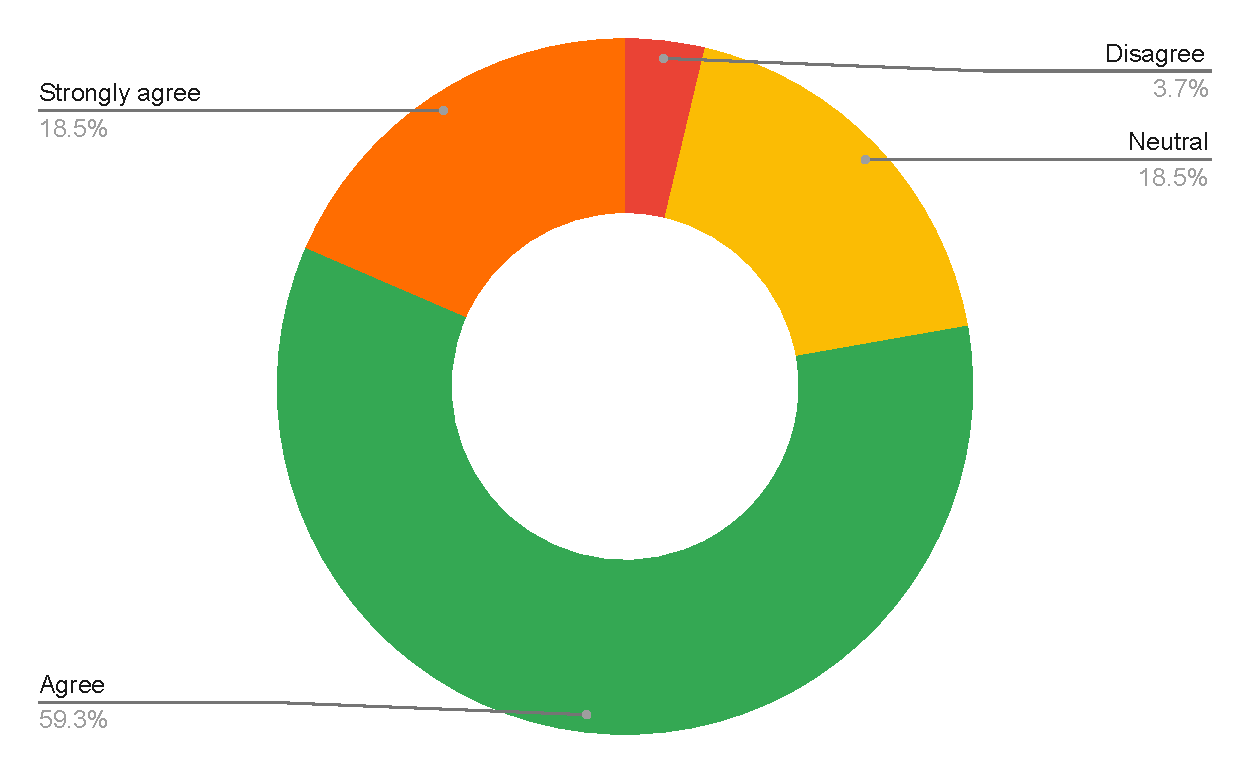
\includegraphics[width=13cm]{thesis/paper/images/p2u_q5.pdf}
  \textbf{Question (End-user survey):} I would benefit from the guaranteed accessibility aspect of Intertext
\end{figure}

\begin{figure}[H]
  \centering
  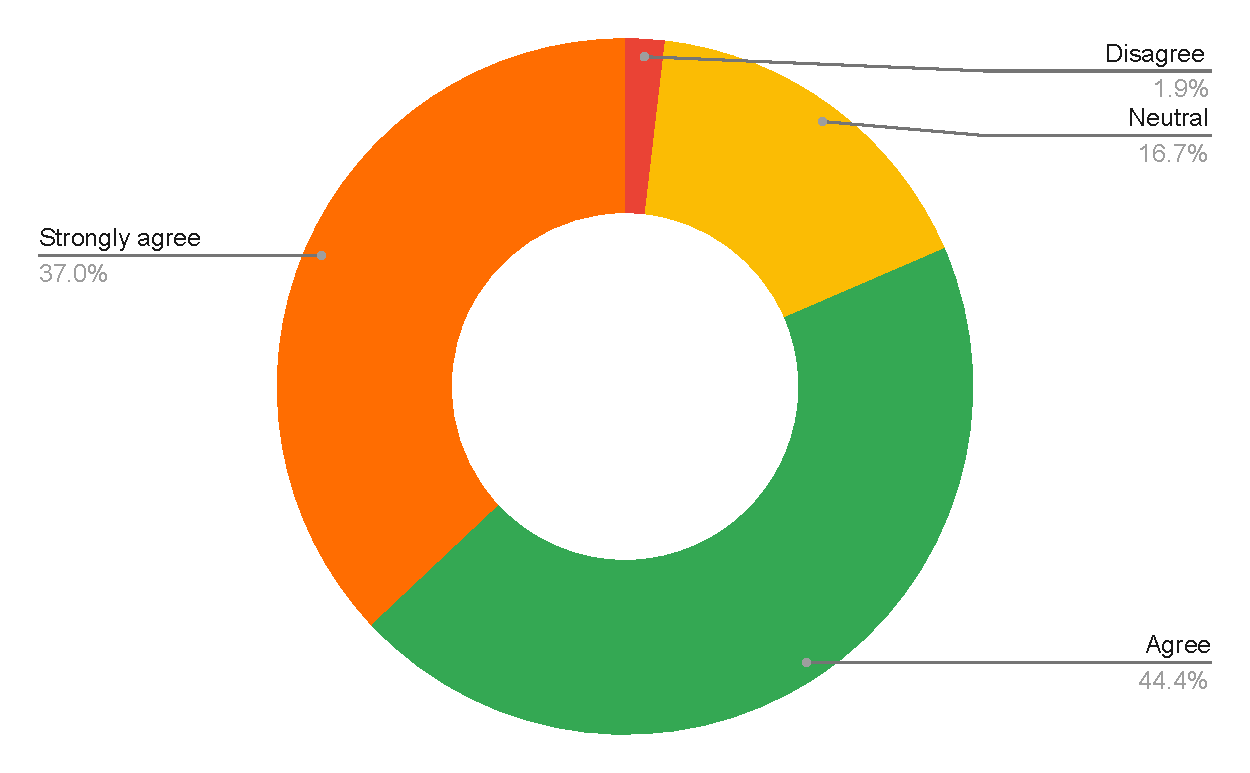
\includegraphics[width=13cm]{thesis/paper/images/p2u_q6.pdf}
  \textbf{Question (End-user survey):} I prefer customisability over variability
\end{figure}

\begin{figure}[H]
  \centering
  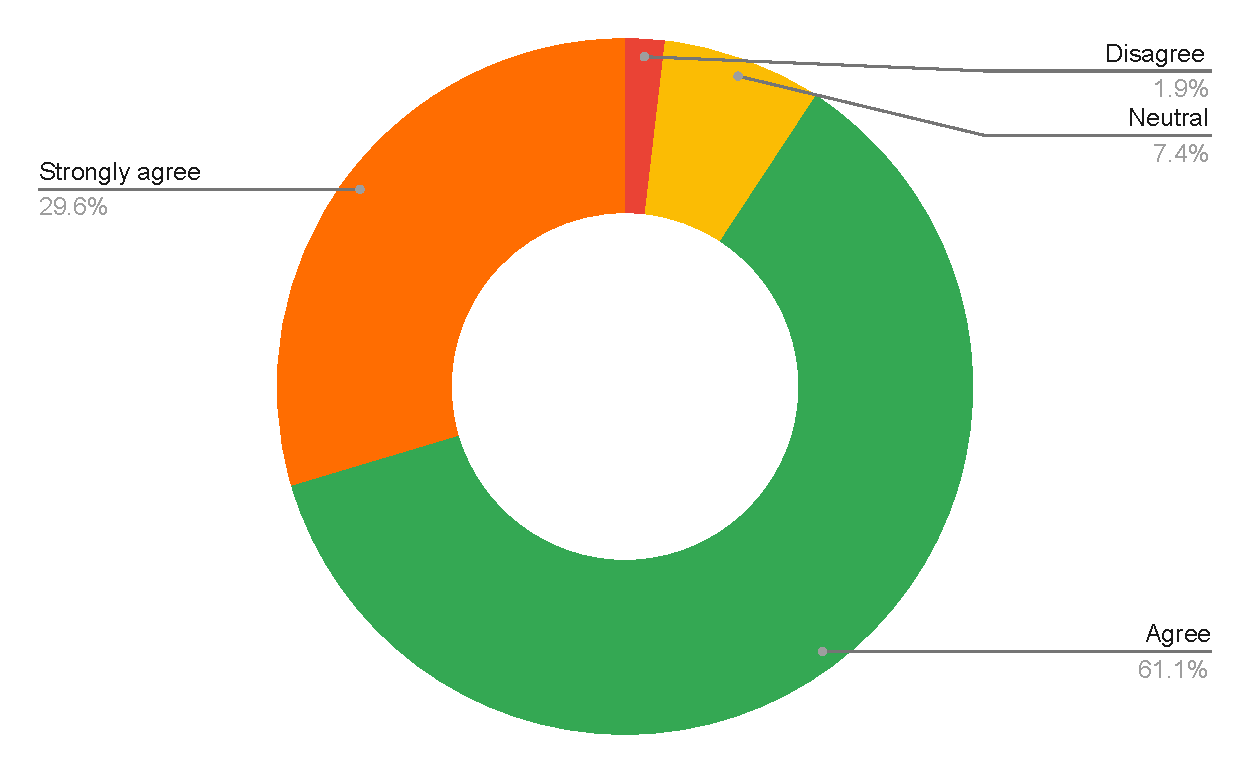
\includegraphics[width=13cm]{thesis/paper/images/p2u_q7.pdf}
  \textbf{Question (End-user survey):} I love that I can create my own theme OR chose a theme I like that applies for all applications
\end{figure}

\begin{figure}[H]
  \centering
  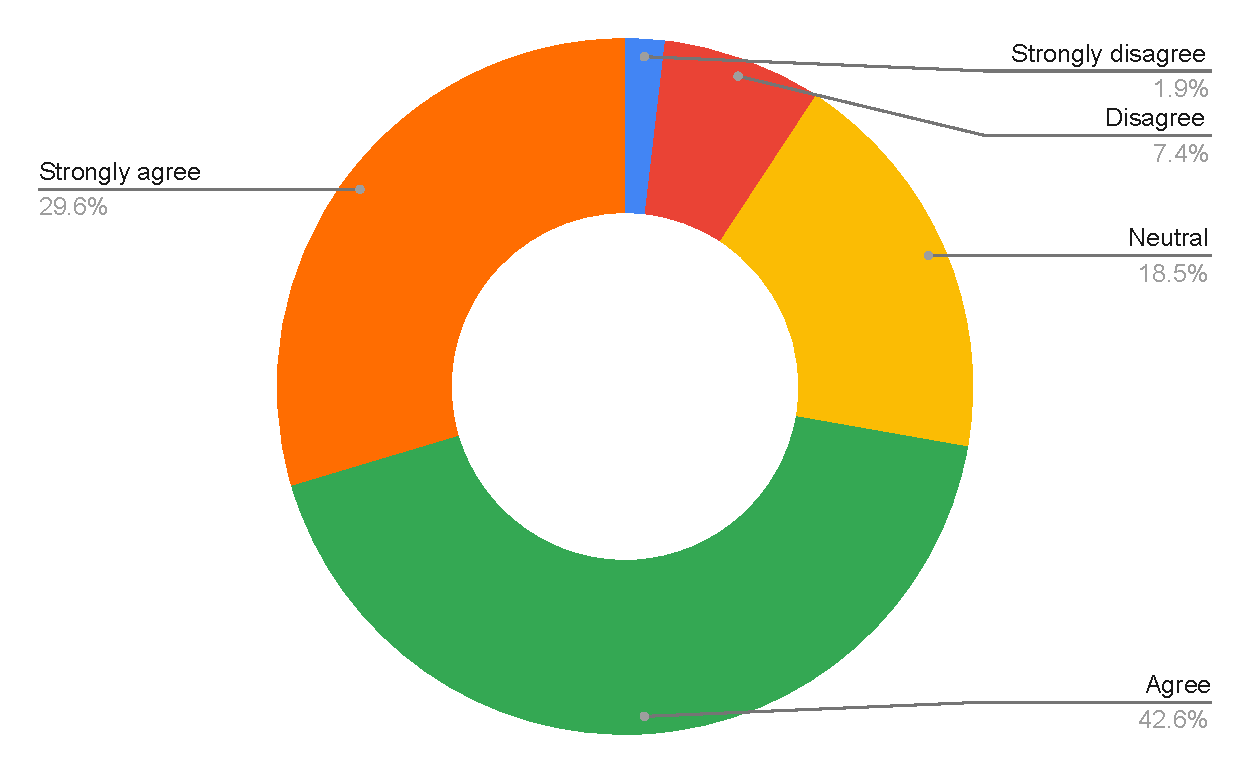
\includegraphics[width=13cm]{thesis/paper/images/p2u_q8.pdf}
  \textbf{Question (End-user survey):} I prefer choosing the look-and-feel I like for all apps, instead of each app having their own look-and-feel
\end{figure}

\begin{figure}[H]
  \centering
  \includegraphics[width=13cm]{thesis/paper/images/p2u_q9.pdf}
  \textbf{Question (End-user survey):} I would be interested in seeing applications running natively on alternative platforms/devices (i.e. other than desktop/mobile - such as wearables, command line interfaces etc.)
\end{figure}

\begin{figure}[H]
  \centering
  \includegraphics[width=13cm]{thesis/paper/images/p2u_q10.pdf}
  \textbf{Question (End-user survey):} If all devices/platforms/environments supported all applications that I use natively, it would increase the use of my other devices.
\end{figure}

\begin{figure}[H]
  \centering
  \includegraphics[width=13cm]{thesis/paper/images/p2u_q11.pdf}
  \textbf{Question (End-user survey):} I would prefer guaranteed privacy and security over rich front-end functionality
\end{figure}

\begin{figure}[H]
  \centering
  \includegraphics[width=13cm]{thesis/paper/images/p2d_q1.pdf}
  \textbf{Question (Developer survey):} I would prefer using IUIDL over building my own components from scratch with the cost of adding cross-platform support
\end{figure}

\begin{figure}[H]
  \centering
  \includegraphics[width=13cm]{thesis/paper/images/p2d_q2.pdf}
  \textbf{Question (Developer survey):} I would prefer using IUIDL over building my own components from scratch with the cost of making them accessible
\end{figure}

\begin{figure}[H]
  \centering
  \includegraphics[width=13cm]{thesis/paper/images/p2d_q3.pdf}
  \textbf{Question (Developer survey):} I would prefer using IUIDL over building my own components from scratch with the cost of maintenance
\end{figure}
% !TEX root = ../thesis.tex

\chapter{Discussion} \label{discussion}

In this thesis, we presented Intertext and the core technologies we developed for this project. We first talked about IUIDL, an XML-based description language that can be used to create generic descriptions of fully functional front-ends without specifying any kind of device or style constraints. Then, we introduced Intertext clients, native applications for the web and several platforms that can render IUIDL natively and effectively taking host environment and user preferences into account. We also clarified how IUIDL can be assembled on the server side based on custom business logic and be served from an endpoint. We provided RecipeApp to serve as an example.

\section{Problem Statement}

In the \nameref{problemStatement} section, we listed the problems we are intending to address with the Intertext project. We grouped these problems under two main categories; problems that are affecting end users, and problems that are affecting developers that are building products for their end users.

We created efficient, streamlined, standardised, accessible and customisable components for Intertext applications to be built with. This standardised approach guarantees that every instance of every component looks consistent. This also solves the intrusive advertisement issue as Intertext clients are in full control of the rendering process. While it cannot stop websites from advertising, the advertisements are also subject to these provided UI components, thus eliminating any non-standard attention-grabbing annoyances that users commonly faces. We made sure that these components are fully accessible, guaranteeing the same level of accessibility for all Intertext apps. We allow users to customise these components, solving lack of customisability problem. We eliminated foreign code execution and had Intertext clients be in full control to solve security and privacy issues. Intertext clients expect XML-based messages from Intertext apps; as no code execution takes place, third party applications has no way of accessing or manipulating users device.

As for developers, we minimised the effort of building and maintaining user facing applications. IUIDL is unified and universal, once developers builds and serves their applications, it works natively on all Intertext clients on all platforms/devices. Thus, we removed the need to build different apps for different platforms. The provided Intertext components are all made accessible, lifting this responsibility from the developer. Moreover, we reduced the front-end application development process to assembling and serving IUIDL. It is agnostic of any technology, framework, device, platform; eliminating the maintenance efforts.

\section{Research Question}

In the \nameref{researchQuestions} section we presented the questions that we aimed to answer in this thesis. We asked focused, specific and actionable questions. In this section, we will discuss how we answered these questions, and recap the answers to these questions.

\paragraph{How can we re-imagine front-end, and improve it in such a way that:}
\begin{enumerate}
  \item from the \underline{users perspective} it:
  \begin{enumerate}
    \item \underline{presents a consistent User Experience (UX) ?}
    
    Intertext comes with building blocks that consists of standardised UI components that guarantees every instance of every component looks consistent. This guarantees consistency not only within a single application, but also across different applications and even across different platforms.
    
    \item \underline{works consistently on all supported devices and platforms ?}

    Intertext offers a number of clients for multiple platforms that offers Native experiences; such as Intertext for web, iOS, Android, macOS, Windows etc. Once an Intertext application is built using the building blocks we provide, it can run on every Intertext client on every device.
    
    \item \underline{allow users to customise the look and feel ?}
    
    Thanks to the UI components being standardised, Intertext clients allows users to customise them and/or apply pre-defined themes. With this approach, user decides on how applications across the Intertext client looks and feels like.
    
    \item \underline{guarantees accessibility ?}

    Intertext comes with standardised UI components, that are implemented with full accessibility support. Every application built on Intertext platform uses the same set of UI components, which guarantees the same level of consistent accessibility support for every Intertext application.

    \item \underline{guarantees security and privacy ?}

    Intertexts approach to combat security and privacy vulnerabilities is to take away the ability for applications to execute code on user devices all together. Intertext clients expects applications to implement their business logic on the server side, and only send instructions to them in a text-based and non-executable format. After receiving these instructions as text, Intertext clients only parses them, and no foreign code execution happens. Developers have no influence on the workings of Intertext clients, other than providing simple text-based instructions. Intertext clients are in full control of what happens on users devices, providing a fully secure environment to the user.
    
  \end{enumerate}
  \item from the \underline{developers perspective}, it:
  \begin{enumerate}
    \item \underline{ eliminates the need to create accessible front-end applications ?}

    As we have already established, IUIDL is agnostic of the view layer. Using IUIDL, developers do not implement \dquote{actual UI elements}, they implement descriptions of a UI. Intertext clients are responsible for interpreting and rendering these descriptions in an accessible manner. The accessibility implementations are already handled, without needing any further action from the developer.
    
    \item \underline{eliminates the need to create front-end applications for every} \newline \underline{device/platform ?}

    Once an Intertext application is being served from an endpoint, it works on any Intertext client on any platform. IUIDL is universal, device agnostic, thus applications built on IUIDL are also universal and device agnostic. It's components, commands, even the layout system runs predictably across all devices of all screen sizes and capabilities, lifting concerns arising from cross-platform development from developers plate.
    
    \item \underline{minimises the need to maintain front-end applications ?}

    Building Intertext applications are merely a matter of assembling and serving XML code from server side. Developers do not need a separate front-end project, any existing backend can be used to serve IUIDL. This way, maintenance requirement of Intertext applications are eliminated.
    
    \item \underline{brings product development costs to a minimum ?}

    Building an Intertext application that works natively on all devices and platforms is a matter of assembling and serving IUIDL code from a backend. It removes the need to create and maintain front-end applications, thus bringing down the development costs significantly.
    
  \end{enumerate}
\end{enumerate}

\section{Limitations}

Intertext platform comes with some limitations arises from its nature. While the novel approach enables some advantages that would otherwise not be possible in traditional front-end applications, there are some drawbacks that comes with it. 

\begin{enumerate}

    \item \textbf{Complex front-end Features}: Intertext applications can only transfer IUIDL to Intertext clients, and feature-wise, they are limited with what Intertext clients and IUIDL offer can offer. Therefore, it is not possible to build custom/complex feature-rich front-end applications.

    \item \textbf{Offline Support}: Intertext clients are like web browsers, they make a request to an endpoint, and render the IUIDL code they receive. As a result, Intertext does not offer offline support out of the box. However, it is possible to work around this by creating a locally running IUIDL server that serves the application through a local endpoint, and pointing the Intertext client to it.
    
    \item \textbf{Design and Branding}: Intertext stands as a user-centric platform that gives end users full control of the look-and-feel of applications. IUIDL is designed as a style-agnostic language with this approach in mind. As a result, it is not possible for developers to implement their own branding and/or style system. It is however possible to add their logos or any other visuals.
    
    \item \textbf{Custom Domains and Standalone Applications}: Intertext applications has to live within Intertext clients. Intertext clients can be thought of like a web browser, and Intertext applications like websites. In a similar sense, Intertext applications needs an Intertext client to be rendered. For the Intertext web client, apps has to be rendered under the domain that the Intertext web client hosted at. For instance, if \textit{example.com} were to be rendered at an Intertext client under \textit{intertext.com}, the domain would look something like \textit{intertext.com/?site=example.com}. For mobile platforms, Intertext applications can live under a native Intertext client. And for desktop platforms, Intertext clients can live under a native Intertext Desktop applications. Therefore, Intertext applications cannot be served under their own top-level domain, and they cannot be standalone applications. It should be noted that all these problems can be resolved. For the web, a custom chromium-based browser could be built with an Intertext client built-in to it. And as in the previous example, when users visits \textit{example.com} it would detect IUIDL code received by the web server and it would render it through the built-in Intertext client. For mobile and desktop platforms, custom operating systems can be built (possibly based on Android for mobile, and based on Linux for desktop) with an Intertext client built into it, which can support Intertext applications natively without the need for a wrapper application. Intertext support can also be built in to existing browsers and operating systems as well.
    
\end{enumerate}


\chapter{Conclusion} \label{conclusion}

In the beginning there were the problems (section \ref{problemStatement}) that we laid out. We started our journey with these problems in mind, and came out of it with an outright solution that we believe can effectively change the way front-end applications are built and consumed by the users. Intertext project is still a work in progress, and has a long way to go before it could present itself as a viable solution. But we do believe that this is a step in the right direction, and that it can reach to a level of becoming a standard in building and consuming user facing applications.

\section{Contributions}

In the \nameref{contributions} section, we have listed our projects main contributions. As a recap, here are the main contributions of the Intertext project:

\begin{itemize}
    
    \item \textbf{IUIDL}: We created an XML-based User Interface description language. We designed it to be device and style agnostic. We gave it the ability to not only describe UI elements, but also flow of actions and commands to make the applications interactive.
    
    \item \textbf{Intertext Engine}: We have centralised the entire logic of parsing, handling and rendering IUIDL into one single engine. Intertext clients that are Javascript-based can use the engine directly; and for clients that are not Javascript-based, a wrapper Node.js application can be built to have it communicate based on the requirements. With Intertext engine being used, clients only have to implement the view layer, and the rest is handled by the engine. Given the open source nature of Intertext, the true power can be realised when community-driven Intertext clients are developed that solves specific problems from specific domains that our clients cannot solve. With this in mind, the engine is a crucial aspect that will enable more clients to be built, and that every client works consistently. 
    
    \item \textbf{Intertext Clients}: We aim to create Intertext clients that covers all the mainstream consumer devices and certain use cases. More details on the future of Intertext is discussed thoroughly in the \nameref{futureWork} section, but as of writing of the thesis, we have implemented the Intertext web client. We created a responsive experience so that it can comfortably be used on mobile browsers until native clients are released.
    
    \item \textbf{Concepts and Ideas}: Perhaps the most important contribution of our project is the novelty of some of the concepts we have introduced. UIDL's are not new, it is an active research topic that has many published papers and projects that covers different corners. We took this concept, adopted it to our use case, and created a novel approach to how front-end's are build in order to solve the aforementioned problems.

\end{itemize}


\section{Future Work} \label{futureWork}

Intertext project is a work in progress. At the time of the thesis, we only implemented the core Engine that handles IUIDL syntax, and the web client that utilises it. Also, some of the features of Intertext mentioned throughout the thesis are not yet available but are planned and on the roadmap. With that said, below are some of the future plans for the Intertext project and the clients:

\begin{enumerate}
    \item \textbf{More Intertext Clients}: As of now, we only developed the Intertext web client. But for this project to be meaningful, there needs to be Intertext clients for every major platform. Thus, Intertext clients for mobile platforms (iOS, Android) and also for desktop environments (macOS, Windows, Linux) are planned. Additionally, an Intertext command-line client with a text-based UI is currently under development.
    
    \item \textbf{Themes}: Currently Intertext web client comes with a light and a dark theme. But we plan to build a lot more themes that users can chose from. Moreover, we plan to allow users to create their own themes, and possibly share the themes they have created with other users.
    
    \item \textbf{Media queries}: We plan to add support for media queries to allow users to adjust the layout based on screen dimensions.
    \item \textbf{Refined control on persisted storage}: Intertext client allows applications to store data on users device/browser. We plan to improve this ability, and support more options such as expiration dates.
    
    \item \textbf{Cross-origin requests}: Intertext clients do not allow cross-origin requests. That is, an application served from an endpoint can only make requests to the same endpoint it is served from. However there are some cases that requires requests outside; for instance loading images, videos, resources from CDN servers, embedding content and so on. To enable this, we plan to allow outside requests once the permission is granted by the user. Also for transparency, we plan to create an interface that displays the request history logs to allow users to investigate the data flow.
    
    \item \textbf{Cross-origin storage read}: Intertext clients by default do not allow applications to read what other applications stored. While this is important to ensure privacy, this can also be used in a good way to enhance user experience. For instance, if a user was logged in at \texttt{example.com}, application served at \texttt{blog.example.com} might want to read the stored user token in order to carry out the session. Therefore, we plan to create a permission flow that asks permission from the users for the read request.
    
\end{enumerate}


% Appendix (optional)
\newpage
\appendix
\renewcommand{\chaptermark}[1]{\markboth{\MakeUppercase{\appendixname}\ \thechapter.\ #1}{}}
\chapter{Appendix} \label{App:AppendixA}
\addtocontents{toc}{\protect\setcounter{tocdepth}{0}}

\section{Source Codes}

\begin{itemize}
    \item Intertext source code: \url{https://github.com/oguzgelal/intertext}
    
    \item RecipeApp demo source code: \url{https://github.com/oguzgelal/intertext-backend-demo}
\end{itemize}



\section{State of JS 2020}

\begin{itemize}
    \item Raw data: \url{https://www.kaggle.com/sachag/state-of-js}
    \item Code used to analyse the data: \url{https://gist.github.com/oguzgelal/8032e0b92077d4b2be909061d6182cdc}
\end{itemize}



 

% Bibliography
\bibliographystyle{plainurl}
\bibliography{bibliography} % uses the file bibliography.bib !
 % -------------------------------------------------

\end{document}
